\documentclass[11pt,a4paper]{article}
\usepackage[utf8]{inputenc}
\usepackage[T1]{fontenc}
\usepackage[spanish,es-nodecimaldot]{babel}
\usepackage{lmodern,amsmath,amssymb,graphicx,booktabs,float,xcolor,caption}
\usepackage[margin=2.2cm]{geometry}
\usepackage{url}
\makeatletter\g@addto@macro{\UrlBreaks}{\do\-\do\_\do\.}\makeatother
\urlstyle{tt}\DeclareRobustCommand{\archivo}[1]{\path{#1}}
\usepackage[colorlinks=true,linkcolor=blue!50!black,urlcolor=blue!50!black]{hyperref}
\captionsetup{font=small,labelfont=bf}
\graphicspath{{../figuras/}}
\newcommand{\aviso}[1]{\par\smallskip\noindent\fcolorbox{orange!70!black}{orange!8}{\parbox{\dimexpr\linewidth-2\fboxsep-2\fboxrule}{\small #1}}\par\smallskip}
\newcommand{\tabla}[1]{\input{tablas/#1}}
\newcommand{\tablaancha}[1]{\resizebox{\linewidth}{!}{\input{tablas/#1}}}
% generado por scripts/curva_humedad.py; no editar a mano
\newcommand{\albSecoTesis}{0.702}
\newcommand{\albSeco}{0.645}
\newcommand{\NHumedades}{5}
\newcommand{\humedades}{5, 10, 15, 25, 30~\%}
\newcommand{\secoTesisUfr}{0.000}
\newcommand{\secoTesisFri}{0.988}
\newcommand{\secoTesisTer}{0.973}
\newcommand{\secoTesisEpi}{0.923}
\newcommand{\secoTesisInt}{0.952}
\newcommand{\secoTesisRap}{0.900}
\newcommand{\secoTesisAlt}{0.747}
\newcommand{\albCinco}{0.565}
\newcommand{\UfrCinco}{nan}
\newcommand{\FriCinco}{1.068}
\newcommand{\TerCinco}{1.245}
\newcommand{\EpiCinco}{0.960}
\newcommand{\IntCinco}{0.804}
\newcommand{\RapCinco}{0.764}
\newcommand{\AltCinco}{0.972}
\newcommand{\albDiez}{0.519}
\newcommand{\UfrDiez}{nan}
\newcommand{\FriDiez}{1.073}
\newcommand{\TerDiez}{1.321}
\newcommand{\EpiDiez}{0.882}
\newcommand{\IntDiez}{0.704}
\newcommand{\RapDiez}{0.648}
\newcommand{\AltDiez}{0.889}
\newcommand{\albQuince}{0.486}
\newcommand{\UfrQuince}{nan}
\newcommand{\FriQuince}{1.030}
\newcommand{\TerQuince}{1.348}
\newcommand{\EpiQuince}{0.849}
\newcommand{\IntQuince}{0.631}
\newcommand{\RapQuince}{0.566}
\newcommand{\AltQuince}{0.849}
\newcommand{\albVeinticinco}{0.443}
\newcommand{\UfrVeinticinco}{nan}
\newcommand{\FriVeinticinco}{1.066}
\newcommand{\TerVeinticinco}{1.412}
\newcommand{\EpiVeinticinco}{0.835}
\newcommand{\IntVeinticinco}{0.574}
\newcommand{\RapVeinticinco}{0.458}
\newcommand{\AltVeinticinco}{0.871}
\newcommand{\albTreinta}{0.427}
\newcommand{\UfrTreinta}{nan}
\newcommand{\FriTreinta}{1.036}
\newcommand{\TerTreinta}{1.423}
\newcommand{\EpiTreinta}{0.776}
\newcommand{\IntTreinta}{0.550}
\newcommand{\RapTreinta}{0.423}
\newcommand{\AltTreinta}{0.839}
\newcommand{\ajInta}{0.050}
\newcommand{\ajIntb}{0.453}
\newcommand{\ajIntc}{0.091}
\newcommand{\ajResInt}{0.9}
\newcommand{\ajRapa}{0.087}
\newcommand{\ajRapb}{0.265}
\newcommand{\ajRapc}{0.119}
\newcommand{\ajResRap}{1.0}
\newcommand{\bandaMax}{12}
\newif\ifquince\quincetrue

% generado por scripts/captura_wcd.py; no editar a mano
\newif\ifbalancerapido\balancerapidotrue


\title{Albedo de neutrones de un suelo SoilBS según su humedad\\
\large flujo atmosférico de Bucaramanga sobre suelo seco y húmedo, simulado en MEIGA}
\author{Jaime Betancourt}
\date{26 de octubre de 2026}

\begin{document}
\maketitle

\begin{abstract}
Se simuló en MEIGA el campo de neutrones que baja sobre Bucaramanga (curva ``Baja'' de la tesis) incidiendo sobre el
suelo modelo SoilBS de la tesis, sin tanque, seco y con \humedades{} de agua en masa. Un plano virtual a 5~cm sobre
el suelo cuenta los neutrones que suben, y para cada uno se registra si es el incidente reflejado o uno creado en el
suelo. Las energías se agrupan con la clasificación de la tesis (Tabla~2.2: fríos, térmicos, epitérmicos,
intermedios, rápidos y de alta energía). El suelo seco de MEIGA reproduce el espectro seco de la tesis por debajo de
$\sim$10~MeV (térmicos \secoTesisTer, intermedios \secoTesisInt, rápidos \secoTesisRap); por encima de 20~MeV queda
\secoTesisAlt{} de la tesis, una diferencia entre las dos simulaciones y no un efecto del agua.
Frente al seco de MEIGA, con los mismos neutrones de entrada, la humedad baja los neutrones intermedios
(1~eV--10~keV) a \IntCinco, \IntDiez, \ifquince\IntQuince, \fi\IntVeinticinco{} y \IntTreinta{} (5, 10, \ifquince 15,
\fi 25 y 30~\%), y los rápidos (10~keV--20~MeV) todavía más (\RapCinco{} a \RapTreinta); los térmicos suben un
25--42~\%. Dentro del suelo, con 30~\% de
agua cada neutrón incidente choca el doble de veces (16.3 frente a 8.5 colisiones elásticas), se crean menos neutrones
(2.2 frente a 3.4 por neutrón inyectado) y el hidrógeno pasa a hacer el 66~\% de las capturas (14~\% en seco). La caída sigue la forma de Desilets et al.~\cite{Desilets2010},
$a_1 + a_0/(\theta_g + a_2)$, con parámetros propios (residuos $\leq\ajResRap$~\%); con los de la literatura
difiere hasta 0.05. La banda de 10~meV a 10~eV, con la que la tesis alimentó el tanque, cambia apenas un \bandaMax~\%: para
la curva de calibración hay que usar el espectro completo: plegado con la eficiencia del WCD de 1~meV a 1~GeV, las
cuentas bajan entre seco y 30~\% un 8.6, 9.4, 9.9 y 10.4~\% (agua pura, 2.5, 5 y 10~\% NaCl), y hasta 12.7~\% con NaCl y una
ventana de carga; la sensibilidad crece con la concentración de sal. El coeficiente de captura del neutrón incidente
en el WCD va de 17.4~\% (1~meV) a un máximo de 62.8~\% en 5~MeV en agua pura (20.6 y 65.6~\% con 2.5~\%, 23.4 y 66.6~\%
con 5~\% y 28.1 y 68.8~\% con 10~\% NaCl) y cae por
debajo del 7~\% desde 100~MeV, donde dominan las interacciones inelásticas y la transmisión. La simulación directa en el tanque, con los
neutrones que suben entrando por la base y por el costado (70~\%), confirma la curva y la hace algo más sensible: 10.0, 10.9, 11.3 y 11.6~\%
(agua pura, 2.5, 5 y 10~\% NaCl) entre seco y 30~\%.
\ifquince\else Falta la corrida con 15~\% de agua, que completará la curva.\fi
\end{abstract}
\tableofcontents

\section{Simulación}
\paragraph{Entrada.} 200\,000 neutrones tomados al azar (semilla 20261023) de los 1\,111\,010 que \emph{bajan} en
\archivo{all_bga_neutron_35.shw}, el flujo en la superficie de Bucaramanga de la tesis, con su energía y dirección
originales (de 0.09~meV a 123~GeV; 58~\% por encima de 20~MeV; $\langle\cos\theta\rangle = 0.81$). Se inyectan con
distribución uniforme en $x, y \in [-8.5, 8.5]$~m, a 6~cm sobre el suelo.

\paragraph{Suelo.} SoilBS de la tesis (cap.~3, Etapa~III; 14 elementos, 2.7~g/cm$^3$), de $20\times20\times1$~m,
con la superficie en $z=0$ y sin tanque (parche \archivo{Parche-suelo-SoilBS}, variables \texttt{MEIGA\_SUELO\_W} y
\texttt{MEIGA\_SIN\_TANQUE}). El suelo húmedo es la mezcla SoilBS + agua con fracción másica $w$ y densidad
$\rho = (w/1 + (1-w)/2.7)^{-1}$; $\theta_g = w/(1-w)$ es la humedad gravimétrica y $\theta_v = w\rho$ el agua en volumen.

\paragraph{Física y conteo.} \texttt{QGSP\_BERT\_HP\_NoThermal} (sin S($\alpha,\beta$)). Se sigue cada paso de cada
neutrón y se cuentan los cruces de un plano a 5~cm sobre el suelo, hacia abajo y hacia arriba, como el plano de la
tesis. El archivo de entrada equivale a \textbf{1~m$^2$ y 12~h} (43\,200~s), como en la tesis: los 1\,111\,010
neutrones que bajan dan $J_\downarrow = 25.7$~n\,m$^{-2}$\,s$^{-1}$, y el flujo que sube es (cruces hacia arriba /
neutrones incidentes) $\times J_\downarrow$. Los cocientes entre suelos no dependen de esa normalización.

\paragraph{Verificación del tiempo de exposición.} En ARTI cada archivo de secundarios corresponde a 1~m$^2$ y al tiempo
$t$ con que se lanza la simulación (opción \texttt{-t}; el número de primarios es $N = \pi\,\Delta S\,\Delta t\int j(E)\,dE$)
\cite{Arti2022,Asorey2018}. La corrida \texttt{Salida\_BGA\_300} del repositorio del taller de ARTI de 2025
\cite{SarmientoCano2025repo} se hizo para Bucaramanga a 956~m, sobre 1~m$^2$ y con $t = 300$~s: tiene 165\,232
secundarios, es decir 551~m$^{-2}$\,s$^{-1}$, como los 540~m$^{-2}$\,s$^{-1}$ que da \cite{Arti2022} para ese sitio, y
3\,923 neutrones (13.1~m$^{-2}$\,s$^{-1}$; CORSIKA solo los sigue por encima de $\sim$50~MeV). Los 569\,038 neutrones que
bajan con más de 50~MeV en \archivo{all_bga_neutron_35.shw} equivalen entonces a \textbf{12.09~h}, y los 25\,545 de más de
1~GeV a 12.10~h. 
%Una versión anterior de este informe usaba 3600~s, lo que daba flujos y tasas absolutas 12 veces mayores; las razones $N/N_0$ no cambian.

\paragraph{Corridas.} Cada humedad usa los 200\,000 neutrones en 4 partes. El suelo seco usa los primeros 50\,000
(modo \texttt{validacion}), que son exactamente los de la parte~1 de cada humedad: los cocientes húmedo/seco se calculan
con esos mismos neutrones de entrada.

\begin{table}[H]
	\centering\footnotesize
	\caption{Resumen de las características de las corridas. Neutrones: incidentes que cruzan el plano hacia abajo.}\label{tab:corridas}
%	\caption{Resumen de las caracteristicas de las corridas (contenedor \texttt{silly\_roentgen}, octubre de 2026). Copias en el disco ADATA 	(\archivo{Corrida-suelo-albedo-resultados}), verificadas frente al contenedor con el número de archivos, los bytes y el 	md5 del listado (manifiesto). Neutrones: incidentes que cruzan el plano hacia abajo.}\label{tab:corridas}
\tabla{corridas}

\end{table}

\section{Clasificación de la energía de los neutrones}\label{sec:clasif}
\subsection{Clasificación adoptada}
Este informe usa la clasificación operativa de la tesis (Tabla~2.2, cap.~2), reproducida en la tabla~\ref{tab:clasif}.
Todos los cocientes, tablas y figuras por región usan esos límites, que caen en la malla de 10 intervalos por década de
los espectros.

\begin{table}[H]
	\centering\small
	\caption{Clasificación de energía operativa de los neutrones adoptada en la tesis (Tabla~2.2) y en este informe. Los
		límites no constituyen una clasificación universal: se establecen para organizar el análisis de las simulaciones. Se
		fundamentan en las clasificaciones de la física de neutrones (Krane~\cite[cap.~12, ``Neutron Physics'',
		pp.~444--477]{Krane1988}), en el estudio de las interacciones de neutrones con la materia
		(Podgoršak~\cite[cap.~9, ``Interactions of Neutrons with Matter'', pp.~429--449]{Podgorsak2010}), y se adaptan al
		contexto de los espectros de neutrones secundarios de origen cósmico (Köhli et al.~\cite[sec.~2.2, pp.~5774--5775,
		fig.~1]{Kohli2015}). Para las bajas energías se consideraron las fuentes de neutrones fríos de la
		IAEA~\cite{IAEA2023Cold}.}\label{tab:clasif}
\begin{tabular}{lc}
\toprule
Designación & Energía del neutrón ($E_n$) \\
\midrule
Ultrafríos & $<0.2$~meV \\
Fríos & 0.2~meV -- 10~meV \\
Térmicos & 10~meV -- 100~meV \\
Epitérmicos & 100~meV -- 1~eV \\
Intermedios & 1~eV -- 10~keV \\
Rápidos & 10~keV -- 20~MeV \\
Alta energía & $>20$~MeV \\
\bottomrule
\end{tabular}

\end{table}

En el campo que sube del suelo casi no hay ultrafríos (menos de 100 cruces por corrida: el espectro empieza en
0.09~meV); se muestran en las tablas de flujo, pero no tienen cociente útil. Los neutrones fríos son el 2~\% del flujo
que sube, los térmicos el 16~\%, los epitérmicos el 6~\%, los intermedios el 24~\%, los rápidos el 49~\% y los de alta
energía el 3~\% (suelo seco de MEIGA).

\subsection{Las clasificaciones de las investigaciones de CRNS}\label{sec:rango}
El método de los neutrones cósmicos para medir humedad (CRNS, \emph{cosmic-ray neutron sensing}) usa un tubo de
$^3$He o BF$_3$ rodeado de polietileno. Cada investigación nombra y delimita las energías a su manera: lo que en CRNS
se llama ``epitérmico'' o ``epitérmico-rápido'' corresponde, en la clasificación de la tesis, sobre todo a los
\emph{intermedios} y al comienzo de los \emph{rápidos}. La tabla~\ref{tab:corresp} reúne las definiciones y su
equivalente.

\begin{table}[H]
	\centering
	\footnotesize\setlength\tabcolsep{4pt}
	\caption{Cómo delimita cada investigación las energías de los neutrones y su equivalente en la clasificación de la
		tesis. Las secciones de~\cite{Kohli2015,Kohli2018} se verificaron en los preprints de arXiv (la fig.~1
		de~\cite{Kohli2015} se discute en la sec.~2.3 del preprint); de~\cite{Desilets2013} solo se consultó el resumen.}\label{tab:corresp}
\begin{tabular}{p{3.6cm}p{5.6cm}p{5.4cm}}
\toprule
Fuente & Denominación y rango & Equivalente en la tabla~\ref{tab:clasif} \\
\midrule
Zreda et al.~\cite{Zreda2012}, sec.~2.1, p.~4081 & térmicos ($\approx$0.025~eV) & térmicos \\
 & epitérmicos ($>0.5$~eV) & epitérmicos (desde 0.5~eV), intermedios y más \\
 & rápidos o de evaporación ($\sim$1~MeV) & rápidos \\
 & de cascada ($\sim$GeV) & alta energía \\
Zreda et al.~\cite{Zreda2012}, sec.~3.1, p.~4085 & el detector moderado responde a los ``epitérmicos-rápidos'' (sin límites) & intermedios y rápidos \\
\midrule
Desilets y Zreda~\cite{Desilets2013}, resumen & energías de detección de $10^0$ a $10^5$~eV & intermedios y rápidos hasta 100~keV \\
\midrule
Köhli et al.~\cite{Kohli2015}, fig.~1 & termalizados ($\sim$meV); epitérmicos/rápidos, ``dominio sensible al agua'' ($\sim$eV--keV); rápidos de evaporación ($\sim$MeV); alta energía ($\sim$100~MeV--GeV) & fríos y térmicos; intermedios; rápidos; alta energía \\
Köhli et al.~\cite{Kohli2015}, sec.~2.3 & la región por debajo de 1~MeV, de choques elásticos, es la más sensible al agua & epitérmicos a rápidos hasta 1~MeV \\
Köhli et al.~\cite{Kohli2015}, sec.~3.3 & ventana de detección de 10~eV a $10^3$~eV & dentro de intermedios \\
\midrule
Köhli et al.~\cite{Kohli2018}, sec.~1 & epitérmicos a rápidos, 1~eV--$10^5$~eV & intermedios y rápidos hasta 100~keV \\
Köhli et al.~\cite{Kohli2018}, sec.~3.1 & respuesta del detector de 0.1~eV a 1~MeV, máxima entre 1 y 10~eV & epitérmicos a rápidos hasta 1~MeV \\
 & ``dominio sensible al agua'', 0.1~eV--0.1~MeV & epitérmicos, intermedios y rápidos hasta 100~keV \\
Köhli et al.~\cite{Kohli2018}, secs.~3.1 y 4.3 & fabricante: 100~eV--10~keV; literatura usual: 0.1--10~keV & intermedios \\
\midrule
Este informe (WCD) & eficiencia de 1~meV a 1~GeV; banda más sensible a la humedad, 0.1--3~MeV & fríos a alta energía; la más sensible, en rápidos \\
\bottomrule
\end{tabular}

\end{table}

La forma de la curva de calibración usada en este informe, $N/N_0 = a_1 + a_0/(\theta_g + a_2)$, y sus parámetros de
la literatura vienen de Desilets et al.~\cite{Desilets2010}.

\paragraph{Relación con este informe.}
\begin{enumerate}
\item La región de los \textbf{intermedios} (1~eV--10~keV) contiene la ventana de los detectores CRNS
(10~eV--1~keV~\cite{Kohli2015}; 0.1--10~keV en la literatura usual~\cite{Kohli2018}). Por eso es la que se compara con
la función de Desilets (sección~\ref{sec:des}).
\item El ``dominio sensible al agua'' de Köhli et al.~\cite{Kohli2018} (0.1~eV--0.1~MeV) abarca los epitérmicos, los
intermedios y el primer tramo de los rápidos.
\item El WCD no es un detector CRNS moderado: su eficiencia sigue de 1~meV a 1~GeV (figuras~\ref{fig:band},
\ref{fig:cap} y~\ref{fig:effbc}) y crece con la energía, así que también cuenta los neutrones rápidos y los de alta
energía.
\item La banda más sensible a la humedad en estas simulaciones, 0.1--3~MeV (figura~\ref{fig:espc}), está dentro de los
\textbf{rápidos}, por encima de la ventana CRNS usual. Es un resultado propio que el WCD puede aprovechar y que los
detectores CRNS, por diseño, ven poco.
\end{enumerate}

\section{Validación: suelo seco de MEIGA frente al de la tesis}
La curva ``Sube'' de la tesis viene del mismo archivo \archivo{all_bga_neutron_35.shw} (los neutrones con $p_z>0$). El suelo seco de MEIGA, con exactamente el mismo montaje que los húmedos, sirve para saber si esa curva puede usarse como referencia.
%La curva ``Sube'' de la tesis viene del mismo archivo \archivo{all_bga_neutron_35.shw} (los neutrones con $p_z>0$), de una simulación cuyas condiciones (partículas que llegan al suelo, física, tamaño del suelo) no están documentadas. El suelo seco de MEIGA, con exactamente el mismo montaje que los húmedos, sirve para saber si esa curva puede usarsecomo referencia.
\begin{figure}[H]\centering
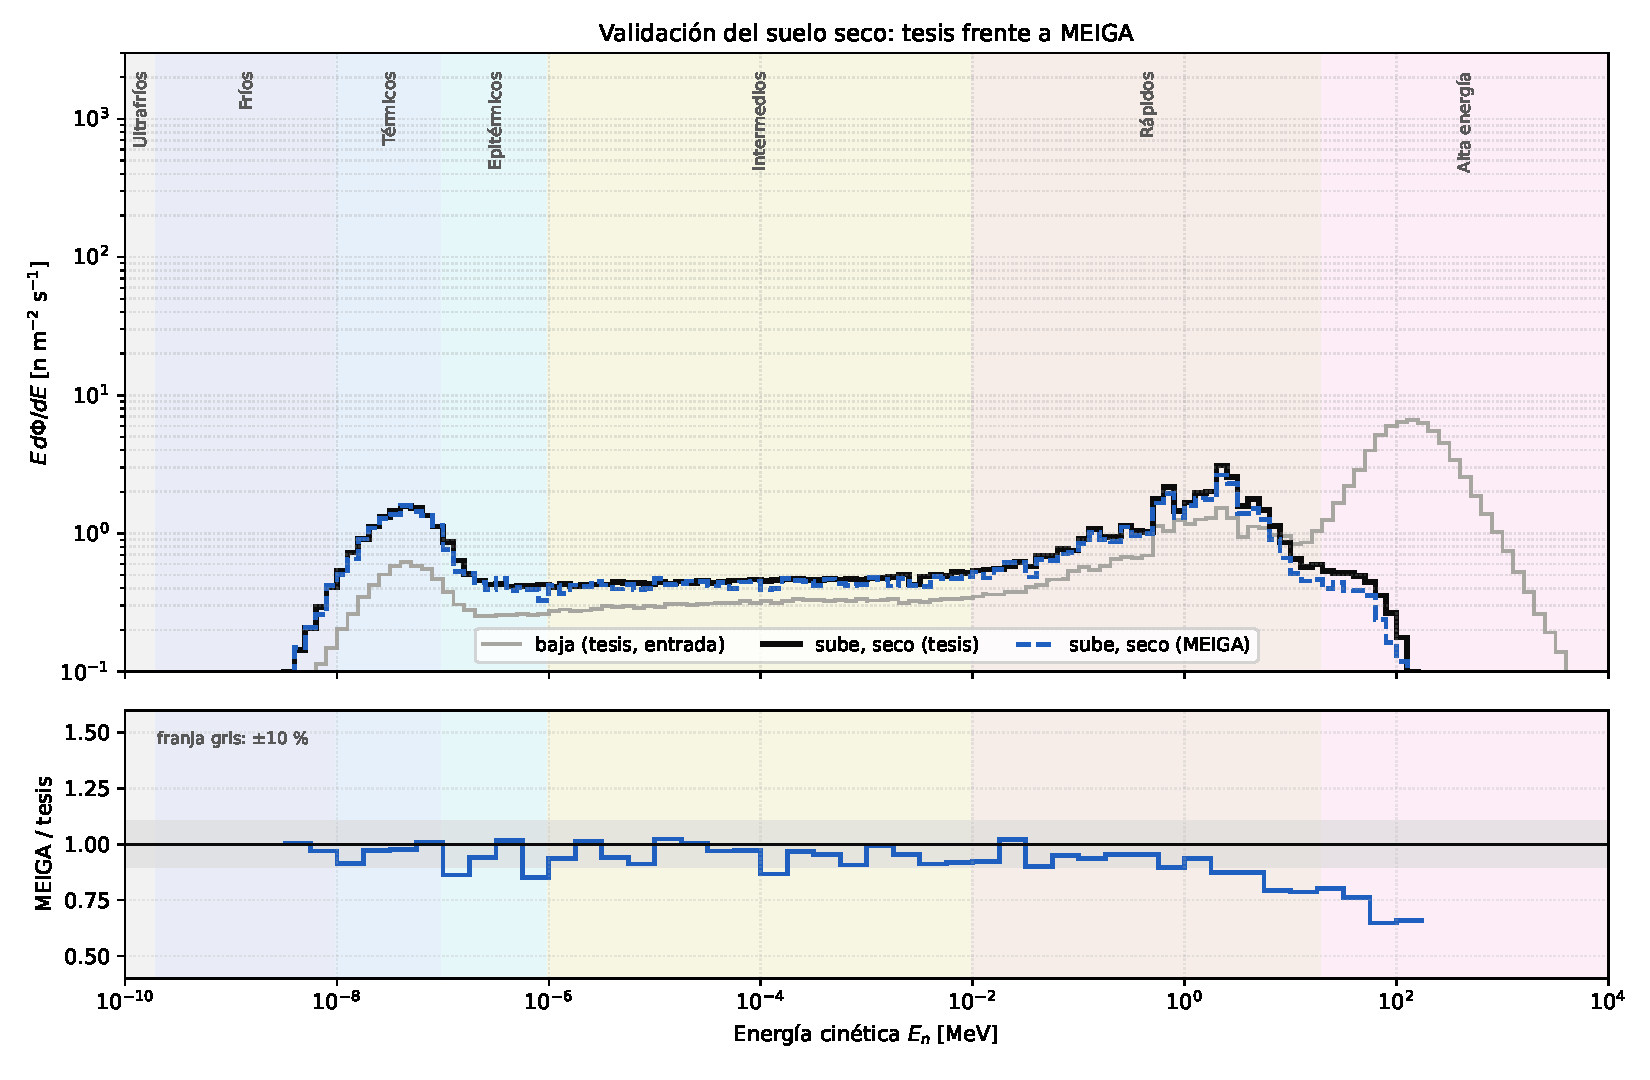
\includegraphics[width=\linewidth]{fig11_validacion_seco.pdf}
\caption{Validación del suelo seco. Arriba: flujo que sube del suelo seco de la tesis (negro) y del de MEIGA (azul, a
trazos), con el flujo que baja en gris. Abajo: cociente MEIGA/tesis por intervalo de energía (4 por década; la franja
gris marca $\pm10$~\%). Coinciden dentro de $\pm10$~\% desde los térmicos hasta $\sim$1~MeV; por encima de 10~MeV el
seco de MEIGA queda entre un 20 y un 35~\% por debajo.}\label{fig:val}
\end{figure}

El albedo total del seco es \albSeco{} neutrones que suben por neutrón que baja (tesis: \albSecoTesis). Por región
(tabla~\ref{tab:clasif}), el seco de MEIGA es \secoTesisFri{} (fríos), \secoTesisTer{} (térmicos), \secoTesisEpi{}
(epitérmicos), \secoTesisInt{} (intermedios), \secoTesisRap{} (rápidos) y \secoTesisAlt{} (alta energía) del de la
tesis. Las dos curvas se superponen hasta $\sim$10~MeV
(figura~\ref{fig:val}); la diferencia está entre 20 y 300~MeV.

\aviso{Conclusión de la validación: la curva seca de la tesis vale como referencia por debajo de 10~MeV. Por encima, el
seco de MEIGA queda un 25~\% por debajo; es posible que la simulación de la tesis incluya neutrones creados en el suelo
por otras partículas de la cascada (protones, piones), que aquí no se inyectan, pero no se pudo verificar. Para el efecto
de la humedad se usa el seco de MEIGA.}

\section{Espectros según la humedad}
\subsection{Esquemas del montaje}
Los tres esquemas siguientes resumen cómo se simula en Geant4 (MEIGA) el intercambio de neutrones entre la atmósfera,
el suelo y el detector. El primero es el montaje de las corridas de albedo con el suelo seco. El segundo es el mismo
montaje con 30~\% de agua y los espectros que bajan y suben. El tercero es el WCD sobre el suelo húmedo, con los
neutrones que entran por la tapa, la base y el costado (sección~\ref{sec:directa}).

\begin{figure}[H]\centering
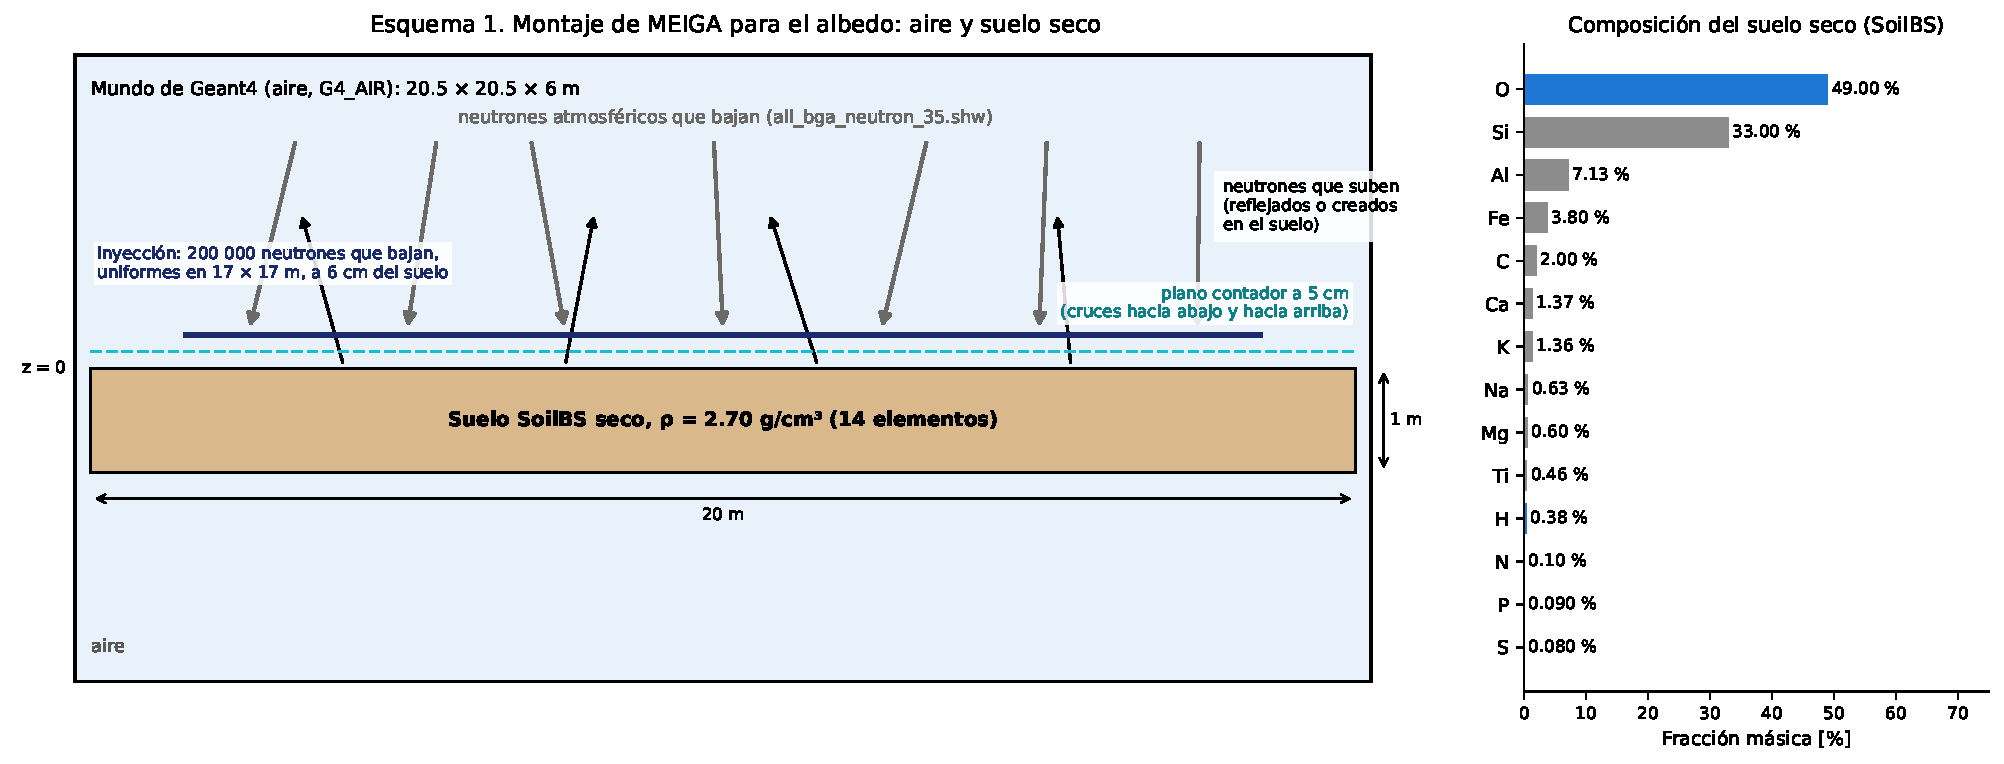
\includegraphics[width=\linewidth]{fig19_esquema_suelo_seco.pdf}
\caption{Esquema~1 (vista lateral, sin escala vertical en la zona de inyección). Mundo de Geant4 de aire
($20.5\times20.5\times6$~m) con el suelo SoilBS seco de $20\times20\times1$~m bajo $z=0$ y su composición másica (14
elementos, 2.70~g/cm$^3$). Los neutrones que bajan se inyectan a 6~cm del suelo en una región de $17\times17$~m; el
plano contador a 5~cm registra los cruces hacia abajo y hacia arriba.}\label{fig:esq1}
\end{figure}

\begin{figure}[H]\centering
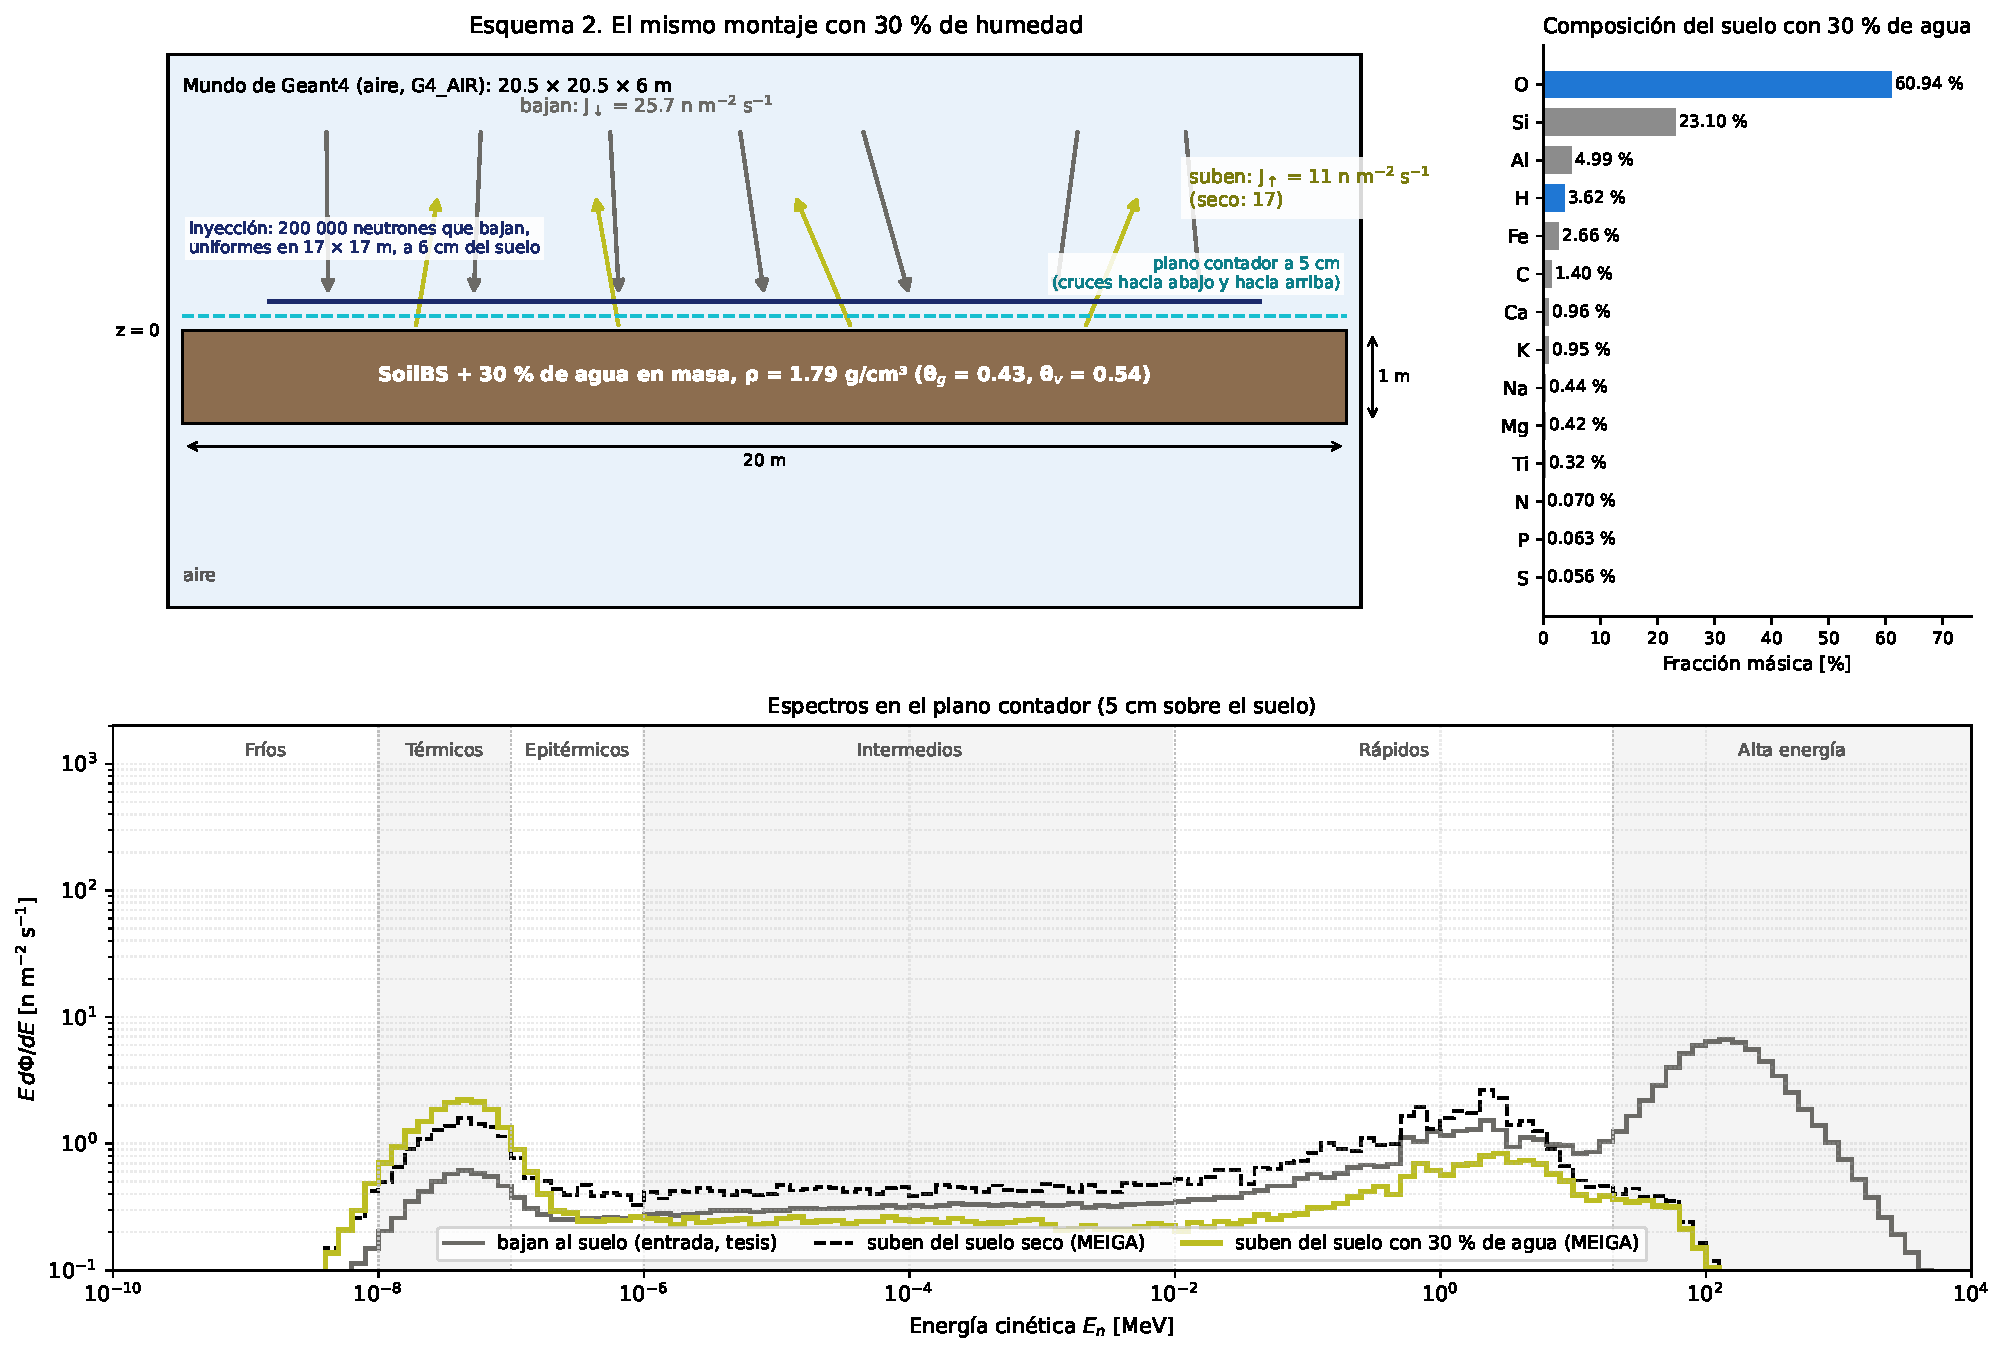
\includegraphics[width=\linewidth]{fig20_esquema_suelo_humedo_espectros.pdf}
\caption{Esquema~2. El mismo montaje con 30~\% de agua en masa (SoilBS 70~\% + agua 30~\%, 1.79~g/cm$^3$): el
hidrógeno pasa de 0.38 a 3.62~\% y el oxígeno de 49.0 a 60.9~\% en masa. Abajo, los espectros en el plano contador: el
que baja (entrada, $J_\downarrow = 25.7$~n\,m$^{-2}$\,s$^{-1}$), el que sube del suelo seco y el que sube con 30~\% de
agua ($J_\uparrow$ = 16.6 y 11.0~n\,m$^{-2}$\,s$^{-1}$), con las regiones de la tabla~\ref{tab:clasif}.}\label{fig:esq2}
\end{figure}

\begin{figure}[H]\centering
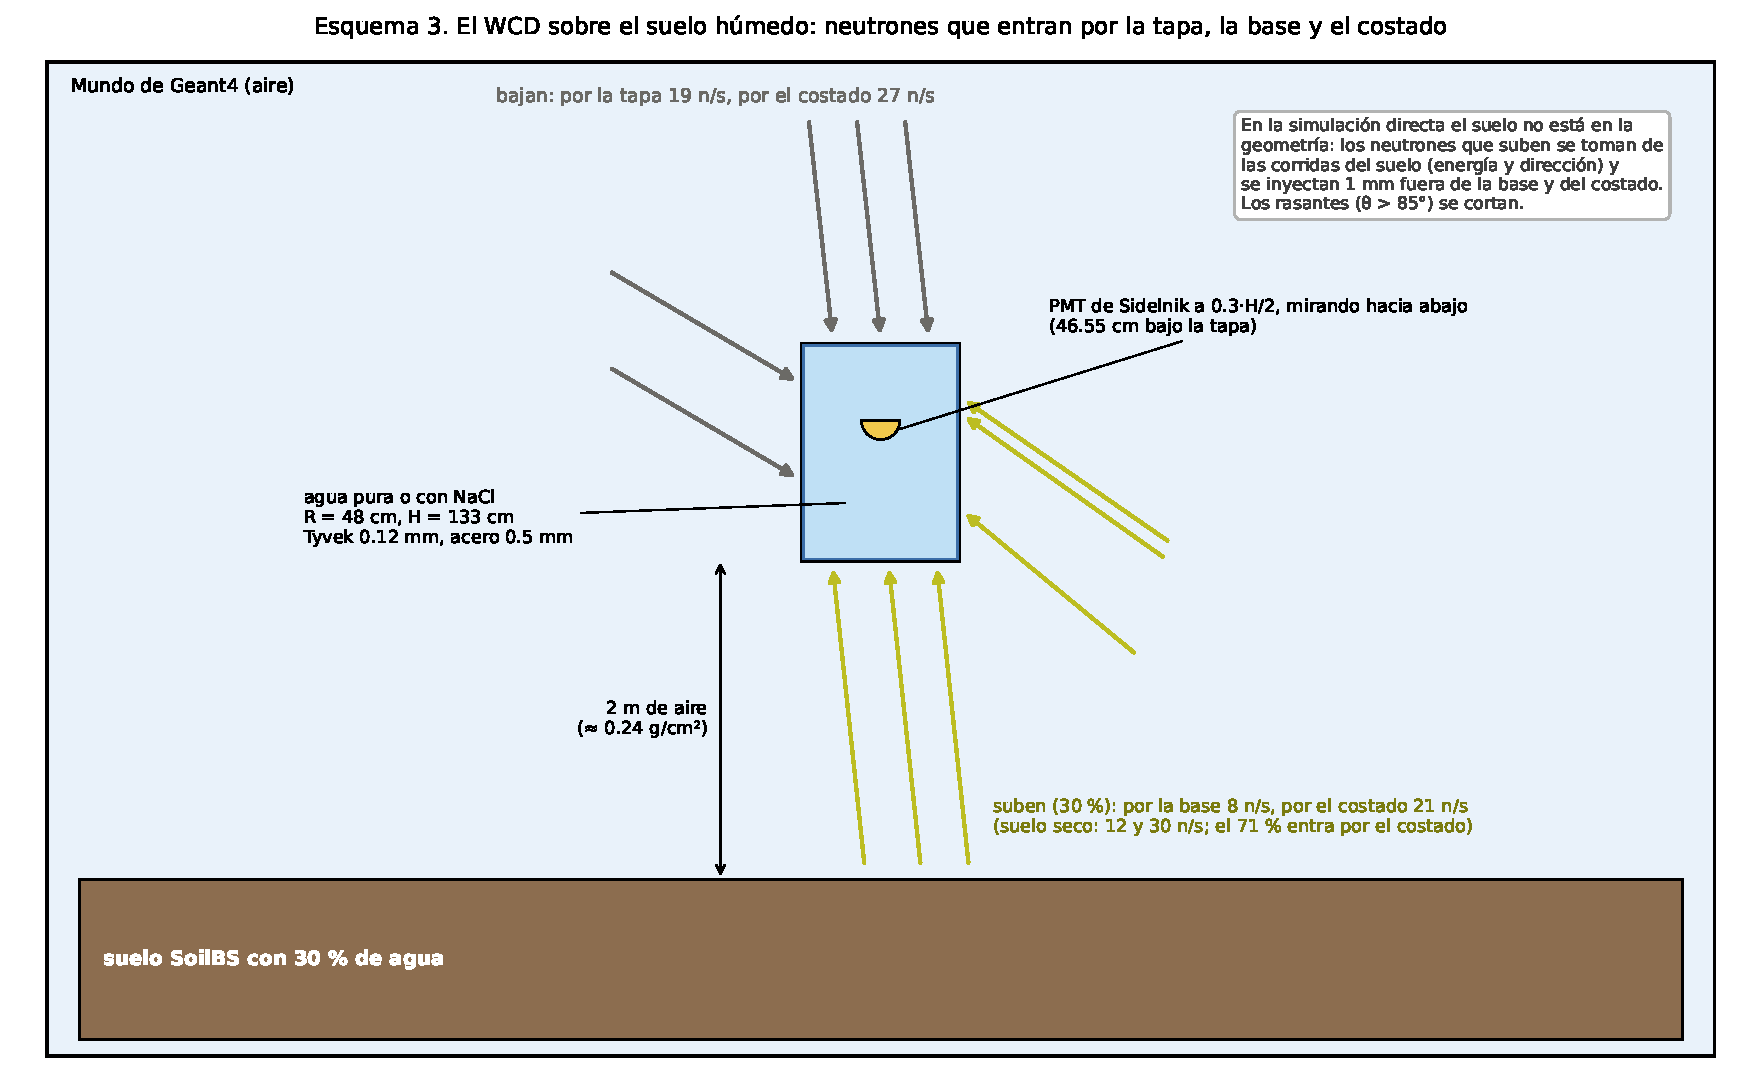
\includegraphics[width=\linewidth]{fig21_esquema_tanque_suelo.pdf}
\caption{Esquema~3. El WCD (SaltyWCD, $R=48$~cm, $H=133$~cm, PMT de Sidelnik a $0.3\,H/2$) a 2~m sobre el suelo con
30~\% de agua. Los neutrones que bajan entran por la tapa (19.0~n/s) y por el costado (27.5~n/s); los que suben, por la
base (8.1~n/s) y por el costado (20.6~n/s; con el suelo seco, 12.3 y 29.6~n/s). En la simulación directa el suelo no está
en la geometría: se inyectan los neutrones que suben de las corridas del suelo, con su energía y dirección.}\label{fig:esq3}
\end{figure}

\subsection{Espectros}
\begin{figure}[H]\centering
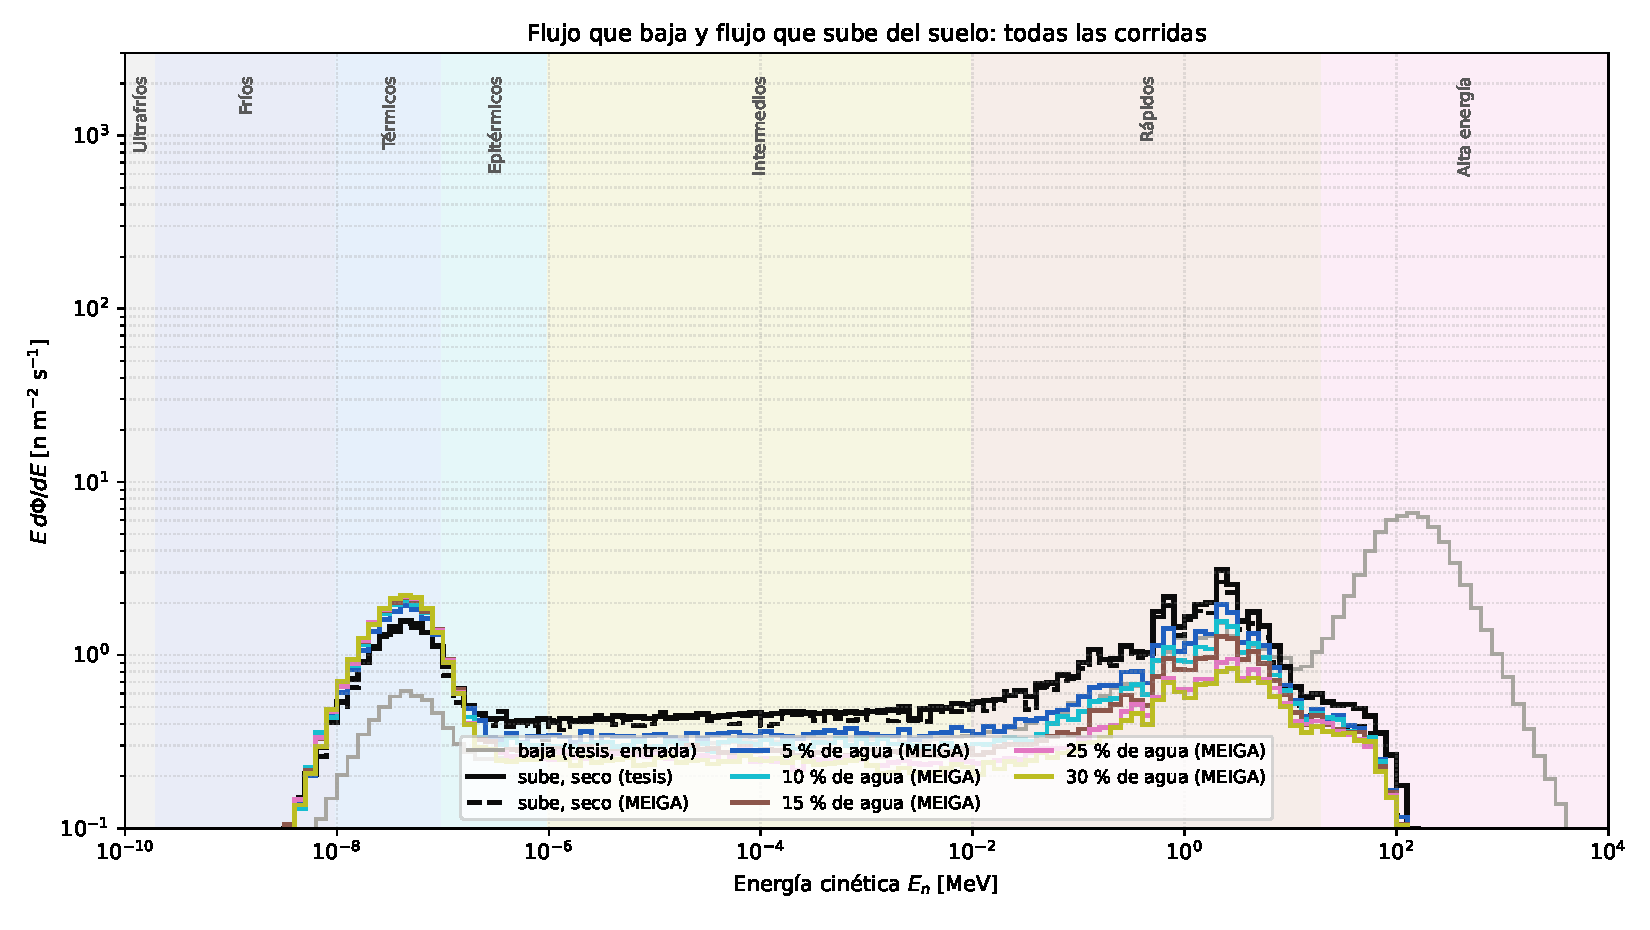
\includegraphics[width=\linewidth]{fig12_todas_las_corridas.pdf}
\caption{Todas las corridas: el flujo que baja (gris), el que sube del suelo seco de la tesis (negro) y de MEIGA (negro,
a trazos), y el que sube con 5, 10, 15, 25 y 30~\% de agua (colores; 200\,000 neutrones por humedad, 50\,000 en el
seco de MEIGA).}\label{fig:esp}
\end{figure}

Las tres figuras siguientes separan esas curvas. Cada humedad tiene un color distinto, el mismo en todas: 5~\% azul, 10~\%
cian, 15~\% marrón, 25~\% rosa y 30~\% oliva (ninguno coincide con los colores de los medios); las referencias secas van en negro y el flujo que baja en gris.

\begin{figure}[H]\centering
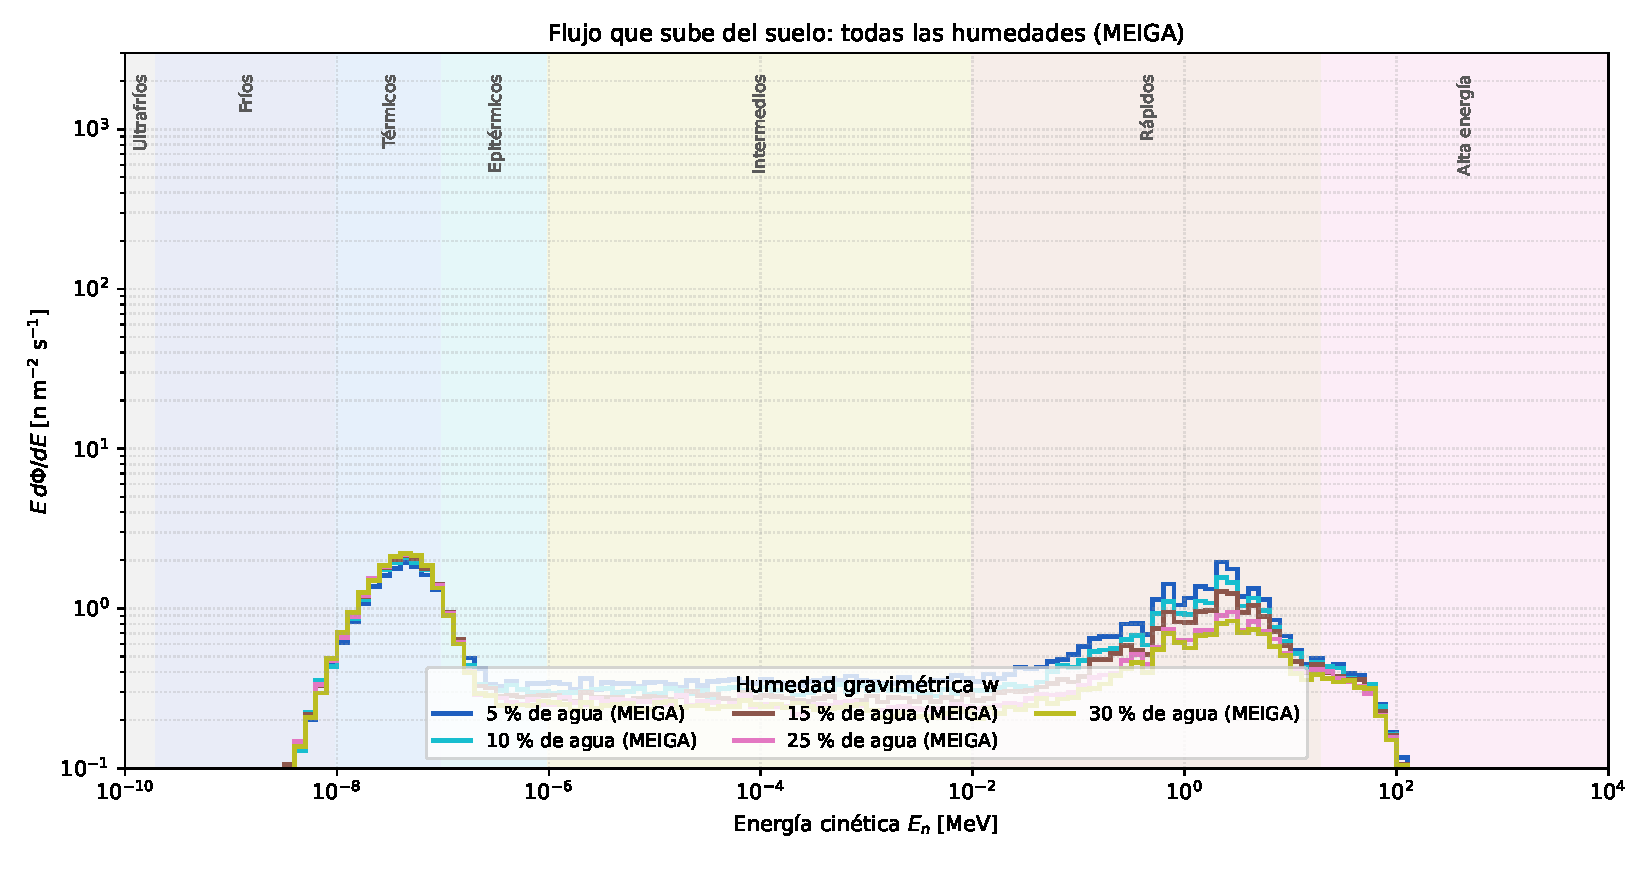
\includegraphics[width=\linewidth]{fig05_espectros_humedades.pdf}
\caption{Solo los suelos húmedos (MEIGA): el agua baja los intermedios y los rápidos, y sube el pico de los
térmicos. Las bandas de fondo son las regiones de la tabla~\ref{tab:clasif}.}\label{fig:hum}
\end{figure}

\begin{figure}[H]\centering
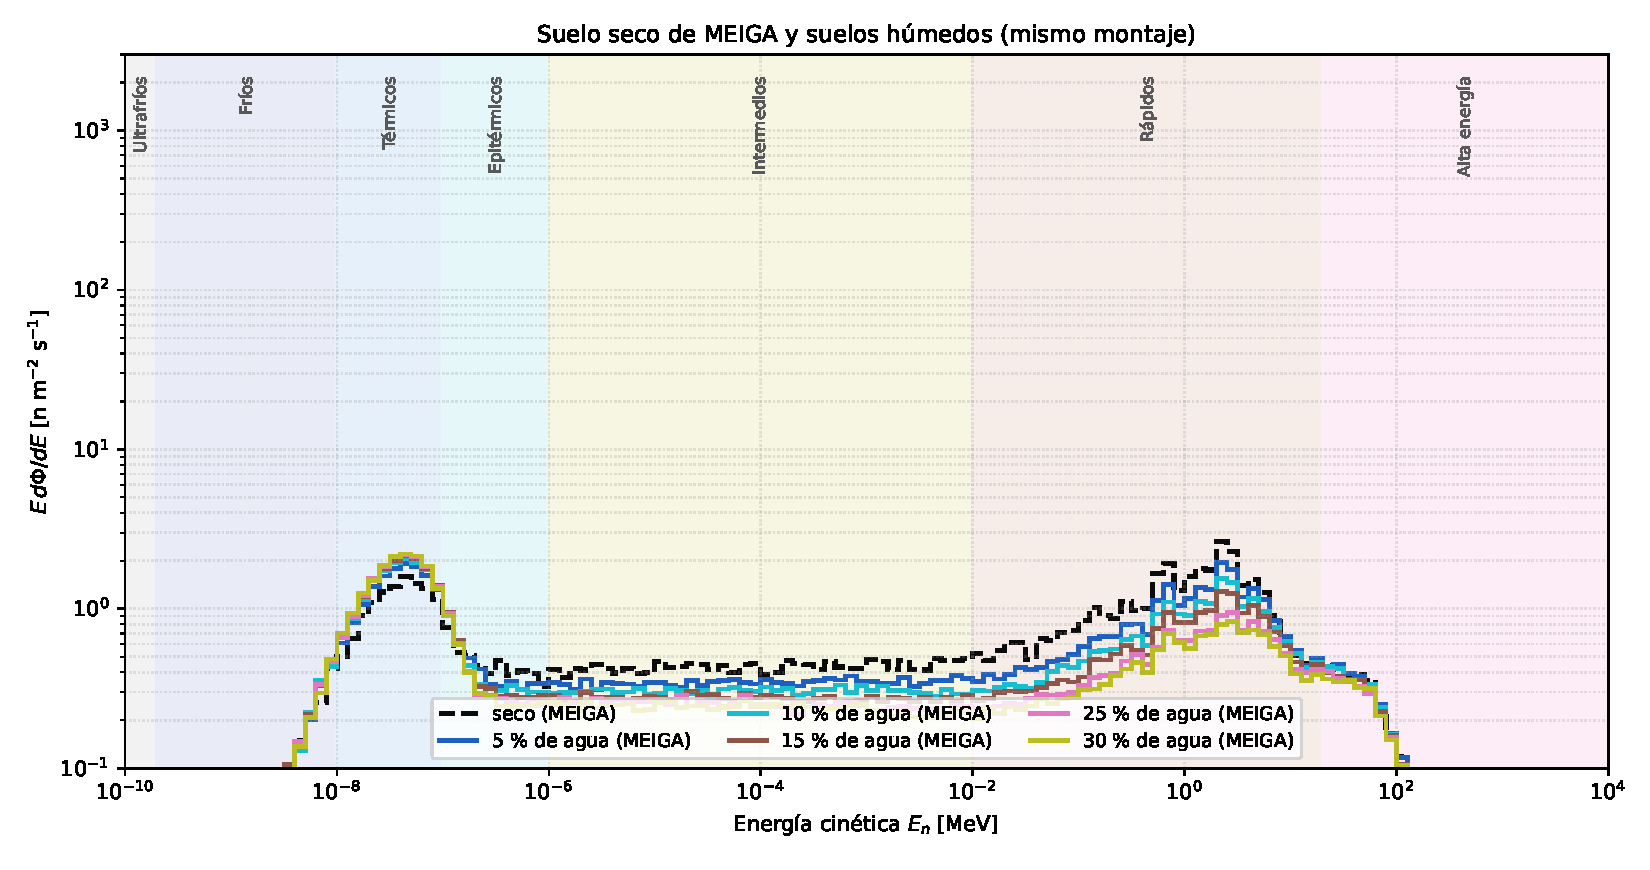
\includegraphics[width=\linewidth]{fig06_seco_meiga_y_humedades.pdf}
\caption{Suelo seco de MEIGA (negro, a trazos) y suelos húmedos: el mismo montaje y la misma física, de modo que las
diferencias son solo efecto del agua.}\label{fig:secom}
\end{figure}

\begin{figure}[H]\centering
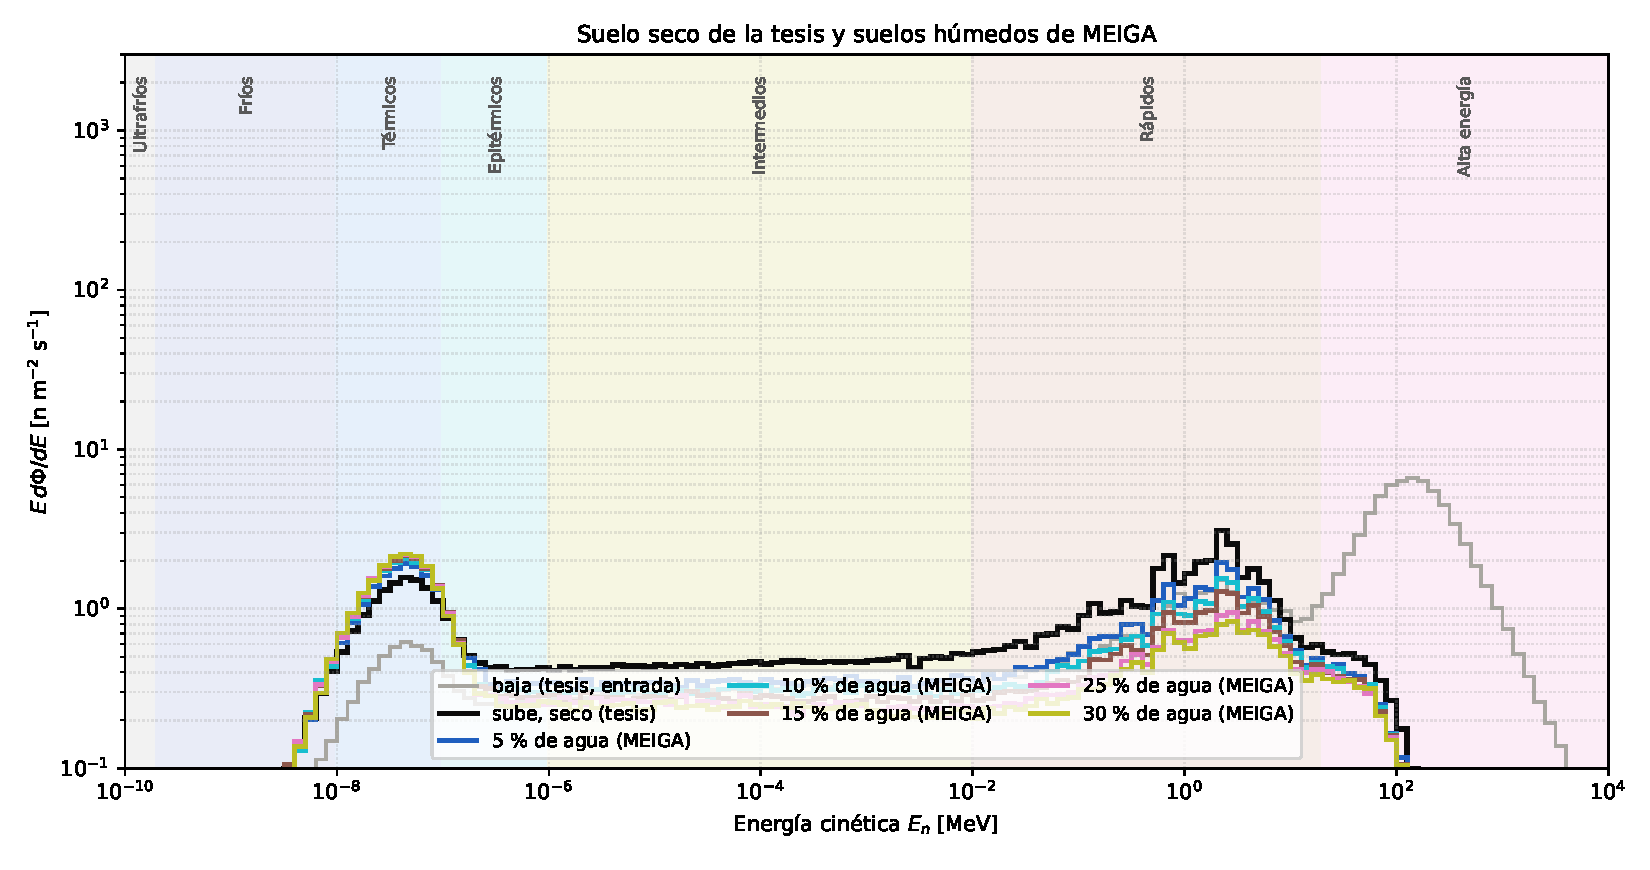
\includegraphics[width=\linewidth]{fig07_seco_tesis_y_humedades.pdf}
\caption{Suelo seco de la tesis (negro) y suelos húmedos de MEIGA; en gris, el flujo que baja (la entrada). Por
encima de 20~MeV el seco de la tesis queda por encima de todas las curvas de MEIGA (sección~2).}\label{fig:secot}
\end{figure}

\begin{table}[H]
	\centering
	\footnotesize\setlength\tabcolsep{4pt}
	\caption{Flujo que sube por región de energía (tabla~\ref{tab:clasif}) [n\,m$^{-2}$\,s$^{-1}$], corridas completas.}\label{tab:flujos}
\tablaancha{flujos}

\end{table}

\section{Efecto de la humedad}
\subsection{Cocientes por región}
\begin{table}[H]
	\centering
	\caption{Flujo que sube con agua dividido por el del suelo seco de MEIGA, por región (tabla~\ref{tab:clasif}; sin
		los ultrafríos, que casi no tienen cruces), con los mismos 50\,000 neutrones de entrada. Errores: estadística de Poisson de los dos conteos (conservadores, porque las entradas son las mismas).
		Albedo: neutrones que suben por neutrón que baja, con esos mismos neutrones. Última columna: la banda de 10~meV a 10~eV.}\label{tab:reg}
	\footnotesize\setlength\tabcolsep{4pt}
\tablaancha{regiones}

\end{table}

\begin{itemize}
\item \textbf{Los intermedios y los rápidos bajan} con la humedad, como en CRNS: a \IntCinco{} y \RapCinco{} con
5~\% de agua, y a \IntTreinta{} y \RapTreinta{} con 30~\%. Los rápidos son la región más sensible. La caída más fuerte
ocurre entre 0 y 10~\%; desde 25~\% la curva se aplana.
\item \textbf{Los epitérmicos} (0.1--1~eV) bajan menos: \EpiCinco{} con 5~\% y \EpiTreinta{} con 30~\%. Están en el
borde entre el frenado y la termalización.
\item \textbf{Los térmicos suben} un 25--42~\% (\TerCinco{} a \TerTreinta) y se estabilizan desde 25~\%: el agua frena
más neutrones hasta el régimen térmico de los que el hidrógeno captura. \textbf{Los fríos} casi no cambian
(\FriCinco{} a \FriTreinta, $\pm$6~\%).
\item \textbf{La alta energía} ($>20$~MeV) casi no depende del agua a 5~\% (\AltCinco) y baja un 11--16~\% a humedad
alta. Con 50\,000 neutrones su error es de $\pm$4~\%.
\end{itemize}

\subsection{Forma de Desilets}\label{sec:des}
La función de calibración usual de CRNS (Desilets et al.~\cite{Desilets2010}) es $N/N_0 = a_1 + a_0/(\theta_g + a_2)$, con
$a_0 = 0.0808$, $a_1 = 0.372$ y $a_2 = 0.115$. Se compara con el cociente de los intermedios de MEIGA, la región que
contiene la ventana de los detectores CRNS (sección~\ref{sec:rango}):

\begin{table}[H]
	\centering\small
\caption{Cociente húmedo/seco de los intermedios (1~eV--10~keV) de MEIGA frente a la función de Desilets con los
	parámetros de la literatura.}\label{tab:des}	
\tabla{desilets}
\end{table}

Con los parámetros de la literatura la diferencia va de $-0.05$ con 5~\% de agua a $+0.03$ con 30~\%: MEIGA cae más
a baja humedad y menos a humedad alta (tabla~\ref{tab:des}). Con la misma forma y parámetros libres, el ajuste a los puntos es excelente (tabla~\ref{tab:aj},
figura~\ref{fig:coc}). La diferencia de parámetros es esperable: Desilets describe las cuentas de un detector
moderado, no el albedo del suelo en una banda fija.

\begin{table}[H]
	\centering\small
\caption{Ajuste de $a_1 + a_0/(\theta_g + a_2)$ a los cocientes de la tabla~\ref{tab:reg} (ponderado por los errores).}\label{tab:aj}	
\tabla{ajustes}

\end{table}

\begin{figure}[H]\centering
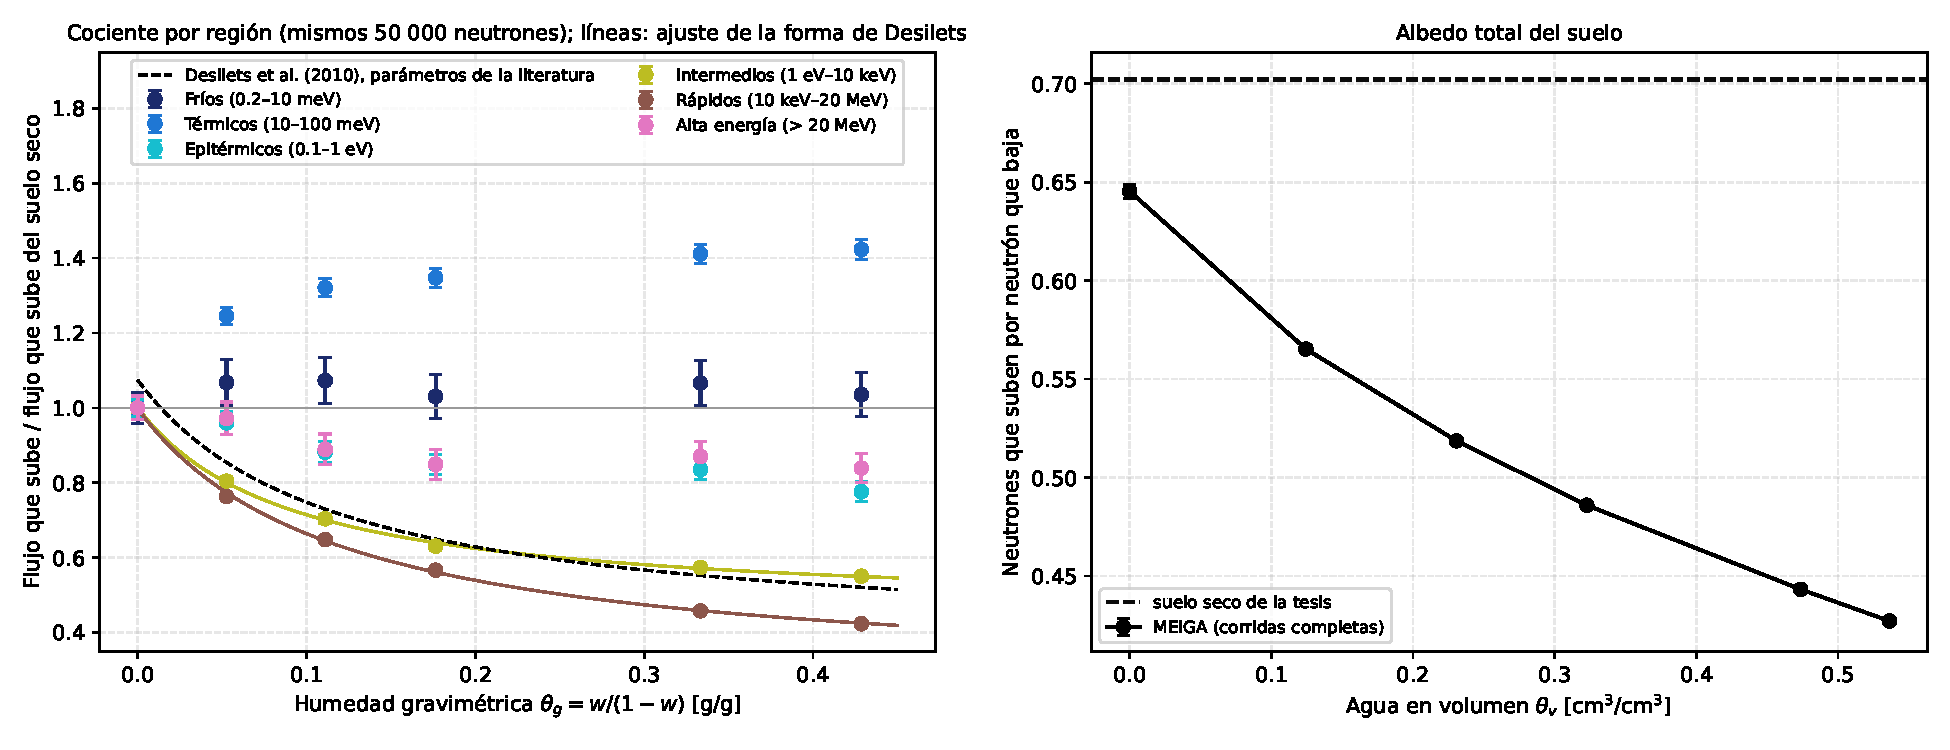
\includegraphics[width=\linewidth]{fig03_cocientes_humedad.pdf}
\caption{Izquierda: cocientes húmedo/seco por región frente a $\theta_g$; líneas continuas: ajuste de la forma de
Desilets; trazos: Desilets con los parámetros de la literatura. Derecha: albedo total frente al agua en volumen.}\label{fig:coc}
\end{figure}

Invertida, la misma relación da la humedad a partir de la razón de neutrones medida,
$\theta_g = a_0/(N/N_0 - a_1) - a_2$, que es la forma en que se usa para calibrar un sensor CRNS
(figura~\ref{fig:inv}).

\begin{figure}[H]\centering
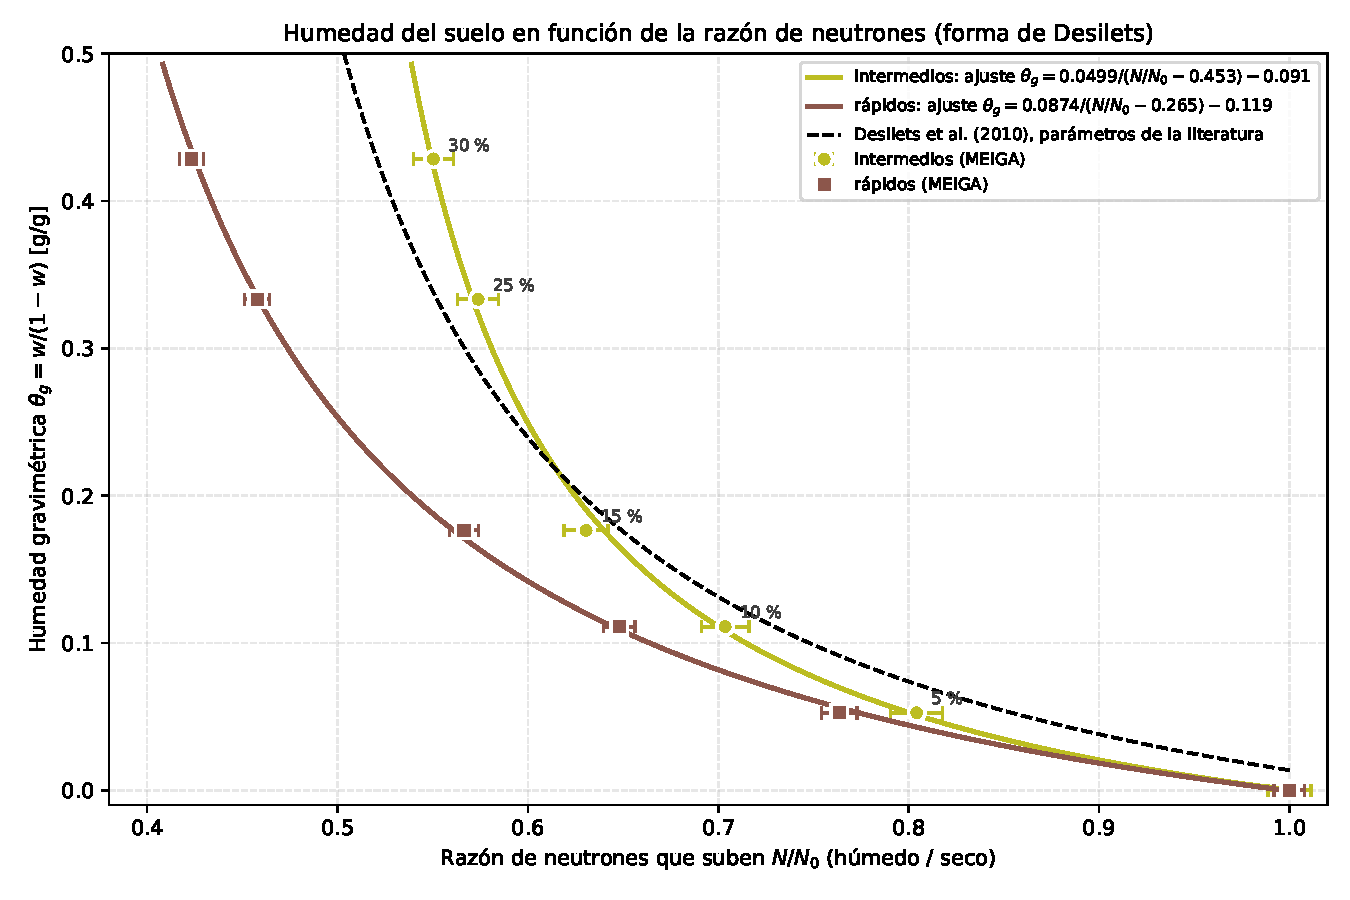
\includegraphics[width=0.85\linewidth]{fig08_humedad_vs_neutrones.pdf}
\caption{Humedad gravimétrica en función de la razón de neutrones que suben $N/N_0$ (húmedo/seco, mismos 50\,000
neutrones), para los intermedios (oliva) y los rápidos (marrón), con su ajuste de la forma de Desilets. En trazos,
la curva de Desilets et al.~\cite{Desilets2010} con los parámetros de la literatura.}\label{fig:inv}
\end{figure}

\subsection{Qué energías son más sensibles}
\begin{figure}[H]\centering
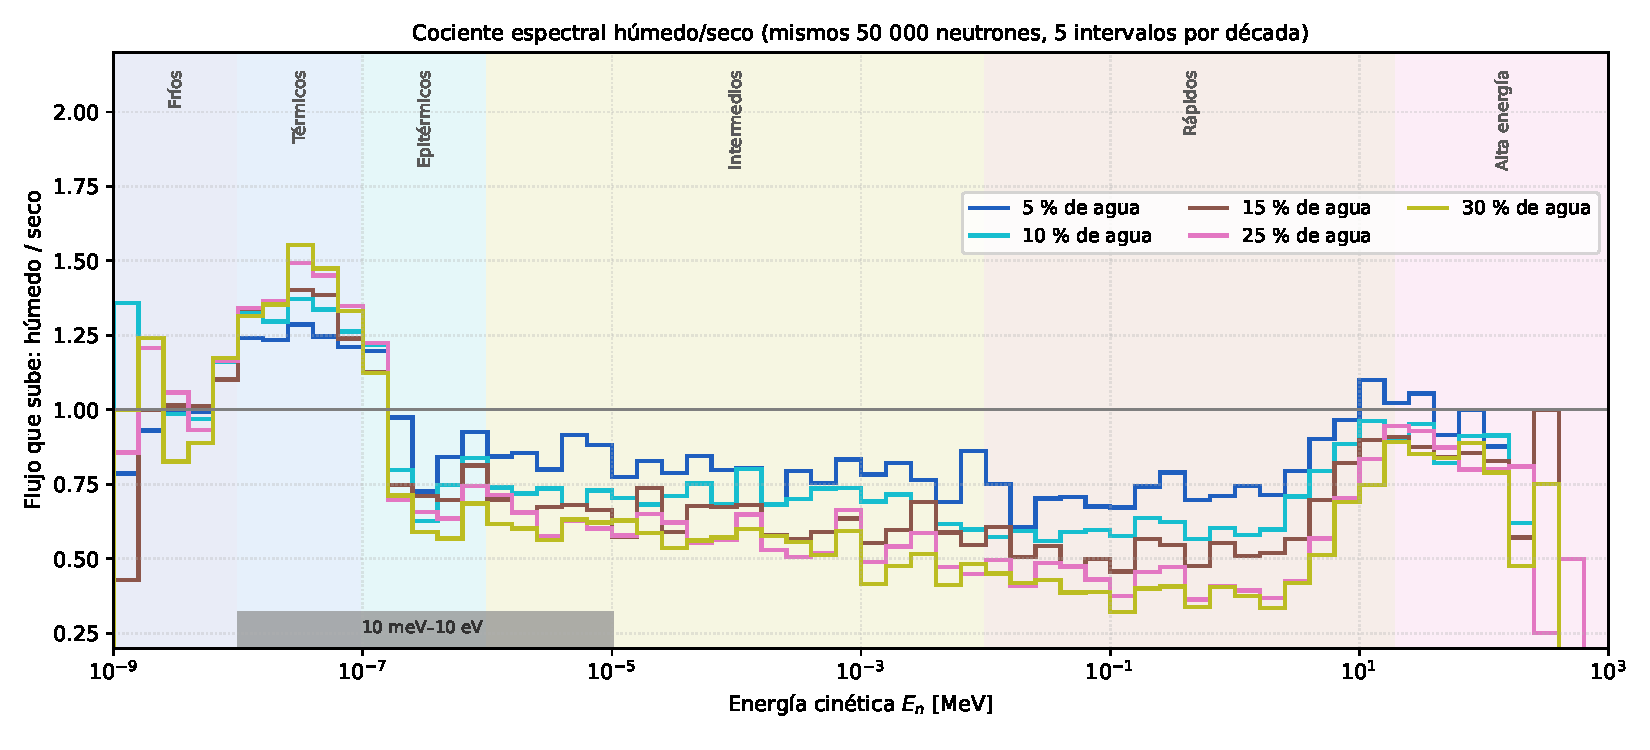
\includegraphics[width=\linewidth]{fig04_cociente_espectral.pdf}
\caption{Cociente húmedo/seco por intervalo de energía (mismos 50\,000 neutrones). La franja gris es la banda de
10~meV a 10~eV.}\label{fig:espc}
\end{figure}

El cociente espectral (figura~\ref{fig:espc}) muestra que la mayor sensibilidad está entre 0.1 y 3~MeV, dentro de
los rápidos, donde el flujo con 30~\% de agua baja a $\approx$0.35 del seco, seguida de los intermedios (0.4--0.6 con
25--30~\%). Entre 10~meV y 0.2~eV (térmicos y comienzo de los epitérmicos) el cociente es \emph{mayor} que 1 (hasta
1.5), y entre 0.2 y 10~eV menor que 1. Por encima de 10~MeV vuelve a acercarse a 1.

\aviso{La banda de 10~meV a 10~eV (\archivo{filtered_neutrons.shw}), la que la tesis inyectó al tanque en la
Sec.~4.5, junta una parte que sube con el agua y otra que baja: en total cambia solo un \bandaMax~\% entre seco y
30~\%. Un detector que solo viera esa banda distinguiría mal la humedad. Para la curva de calibración del tanque hay que
inyectar el espectro completo que sube del suelo, más el que baja.}

\section{Procesos de los neutrones en el suelo}
Esta sección sigue a todos los neutrones dentro del suelo, no solo a los que vuelven a subir. Las cifras son por
neutrón inyectado y salen de \archivo{interacciones-neutrones.tsv} (una línea por interacción) y
\archivo{capturas-neutrones.tsv} (una línea por captura), para las corridas completas.

\begin{table}[H]
	\centering
	\caption{Interacciones dentro del suelo por neutrón inyectado, según el proceso: dispersión elástica
		(\texttt{hadElastic}), dispersión inelástica (\texttt{neutronInelastic}, que destruye el neutrón y crea otros),
		captura (\texttt{nCapture}) y otros. ``Neutrón incidente'' es la traza inyectada; ``secundarios'', todos los
		neutrones creados por ella y sus descendientes.}\label{tab:proc}
	\footnotesize\setlength\tabcolsep{4pt}
\tabla{procesos}

\end{table}

\begin{itemize}
\item El \textbf{neutrón incidente} choca elásticamente 8.5 veces en promedio en el suelo seco y 16.3 veces con
30~\% de agua: el hidrógeno multiplica las colisiones de frenado. Sus dispersiones inelásticas bajan un poco (0.61 a
0.53), porque el suelo húmedo tiene menos núcleos pesados por unidad de volumen.
\item Los \textbf{neutrones secundarios} suman la mayor parte de las interacciones: unas 94--99 colisiones elásticas
por neutrón inyectado. Sus dispersiones inelásticas bajan a la mitad (2.0 a 1.0), porque con agua se crean menos
neutrones rápidos y se frenan antes.
\end{itemize}

\begin{table}[H]
	\centering
	\caption{Destino del neutrón incidente, según su última interacción: capturado; destruido por una dispersión
		inelástica; solo dispersiones elásticas (sale del suelo hacia arriba, por los lados o por el fondo); o ninguna
		interacción. Estos últimos son neutrones de más de $\sim$60~MeV que atraviesan el metro de suelo y salen por el
		fondo.}\label{tab:dest}
	\small
\tabla{destino}
\end{table}

El 54--62~\% de los neutrones incidentes acaba en una dispersión inelástica: el 58~\% de la entrada tiene más de
20~MeV. La fracción capturada sube de 9.0 a 14.1~\%. La de neutrones que atraviesan sin interactuar sube de 0.6 a
2.1~\% porque el suelo húmedo es menos denso (1.79 frente a 2.70~g/cm$^3$): el metro de suelo tiene 179 en vez de
270~g/cm$^2$. Ese límite del modelo (1~m de profundidad) afecta muy poco al albedo, porque esos neutrones se
pierden por abajo.

\begin{table}[H]
	\centering
	\caption{Neutrones creados en el suelo por neutrón inyectado, según el proceso que los creó: dispersión inelástica
		de neutrones (\texttt{neutronInelastic}) y de protones (\texttt{protonInelastic}), captura de hadrones en reposo
		(\texttt{hBertiniCaptureAtRest}) y dispersión inelástica de piones.}\label{tab:crea}
	\footnotesize\setlength\tabcolsep{4pt}
\tabla{creados}

\end{table}

Cada neutrón inyectado crea 3.4 neutrones en el suelo seco y 2.2 con 30~\% de agua; el 95~\% de ellos viene de
dispersiones inelásticas de neutrones (evaporación y $(n,xn)$), y el resto de protones, piones y capturas de
hadrones en reposo. Con agua hay menos núcleos pesados, y por eso menos neutrones de evaporación: es la causa de la
caída de los rápidos (10~keV--20~MeV) que suben.

\begin{table}[H]
	\centering
	\caption{Capturas de neutrones en el suelo: número por neutrón inyectado y reparto por núcleo [\%].}\label{tab:cap}
	\footnotesize\setlength\tabcolsep{4pt}
\tabla{capturas}
\end{table}

Se captura alrededor de un neutrón por neutrón inyectado (1.0--1.1), porque cada incidente crea varios. En el suelo
seco capturan sobre todo el Si (28~\%) y el Fe (25~\%); el H, con solo 0.38~\% en masa, ya captura el 14~\%. Con
agua el hidrógeno domina: 29~\% con 5~\% de agua y 66~\% con 30~\%.

\section{Origen de los neutrones que suben}
\begin{table}[H]
	\centering\small
\caption{Origen de los cruces hacia arriba del plano: el neutrón incidente reflejado, uno creado por dispersión
	inelástica de un neutrón (\texttt{neutronInelastic}: evaporación y $(n,xn)$) u otros procesos (protones, piones,
	capturas de hadrones en reposo).}\label{tab:orig}
\tabla{origen}
\end{table}

En el suelo seco la mayoría de los neutrones que suben son creados en el suelo (56~\%, casi todos por \texttt{neutronInelastic}). Con agua, la fracción de
reflejados crece hasta 66~\% (30~\%), porque los neutrones de evaporación se frenan y se capturan antes de salir.

\section{Curva de calibración del WCD}\label{sec:cal}
\subsection{Método}
El WCD no mide el espectro: cuenta eventos. La humedad se obtiene de cómo cambia el número de cuentas con el agua del
suelo. Para cada suelo se calculan las cuentas esperadas plegando el campo de neutrones con la eficiencia del detector:
\begin{equation}
N(\theta) = A\,t \sum_E \big[\Phi_\downarrow(E) + \Phi_\uparrow(E;\theta)\big]\,\varepsilon(E),
\end{equation}
donde $\Phi_\downarrow$ es el flujo que baja (la curva ``Baja'' de la tesis, el mismo para todos los suelos),
$\Phi_\uparrow(E;\theta)$ el que sube del suelo con humedad $\theta$ (las corridas de este informe), $\varepsilon(E)$ la
fracción de neutrones de energía $E$ que dejan una señal en el PMT, $A=\pi R^2$ la sección del tanque ($R=48$~cm) y $t$
el tiempo de medida. La razón $N(\theta)/N_0$, con $N_0$ las cuentas sobre el suelo seco, es la curva de calibración.

\begin{enumerate}
\item \textbf{Eficiencia de 1~meV a 1~keV:} la de la Campaña~1 (16 energías, 4 medios, $10^5$ neutrones por energía).
\item \textbf{Eficiencia de 1~keV a 1~GeV:} un barrido rápido nuevo, con la misma geometría y física que el barrido de
S($\alpha,\beta$): 8 energías (1, 10 y 100~keV; 1, 5, 20 y 100~MeV; 1~GeV), entre 1\,000 y 10\,000 neutrones, en los
cuatro medios (agua pura y 2.5, 5 y 10~\% NaCl; unas 2~h de cálculo por cada par de medios, con 4 procesos).
\item \textbf{Empalme en 1~keV.} En 1~keV las capturas coinciden con la Campaña~1 (0.332 frente a 0.338 en agua pura;
0.374/0.376, 0.408/0.409 y 0.455/0.454 con 2.5, 5 y 10~\% NaCl), pero la luz detectada es un 6--10~\% menor: el PMT de
Sidelnik del barrido es más pequeño. Para $Q\geq1$ el barrido se multiplica por 1.12, 1.09, 1.09 y 1.07. La curva cambia menos de
0.0004 con o sin ese factor.
\item \textbf{Plegado} con los seis espectros, para tres criterios de cuenta: $Q\geq1$~p.e., $Q\geq5$~p.e.\ y la
ventana $1\leq Q<20$~p.e.
\end{enumerate}

\begin{table}[H]
\caption{Eficiencia del WCD en el barrido rápido (neutrones verticales por la tapa, sin empalme): fracción con
	$Q\geq1$ y $Q\geq5$~p.e., y fracción de eventos con al menos una captura en el agua (de cualquier neutrón, incluidos los
	secundarios; no es el $\eta_{\rm Cap}$ del neutrón incidente de la sección~\ref{sec:cap}).}\label{tab:eff}	
	\centering\small
\tabla{eficiencia_wcd}
\end{table}

\begin{figure}[H]\centering
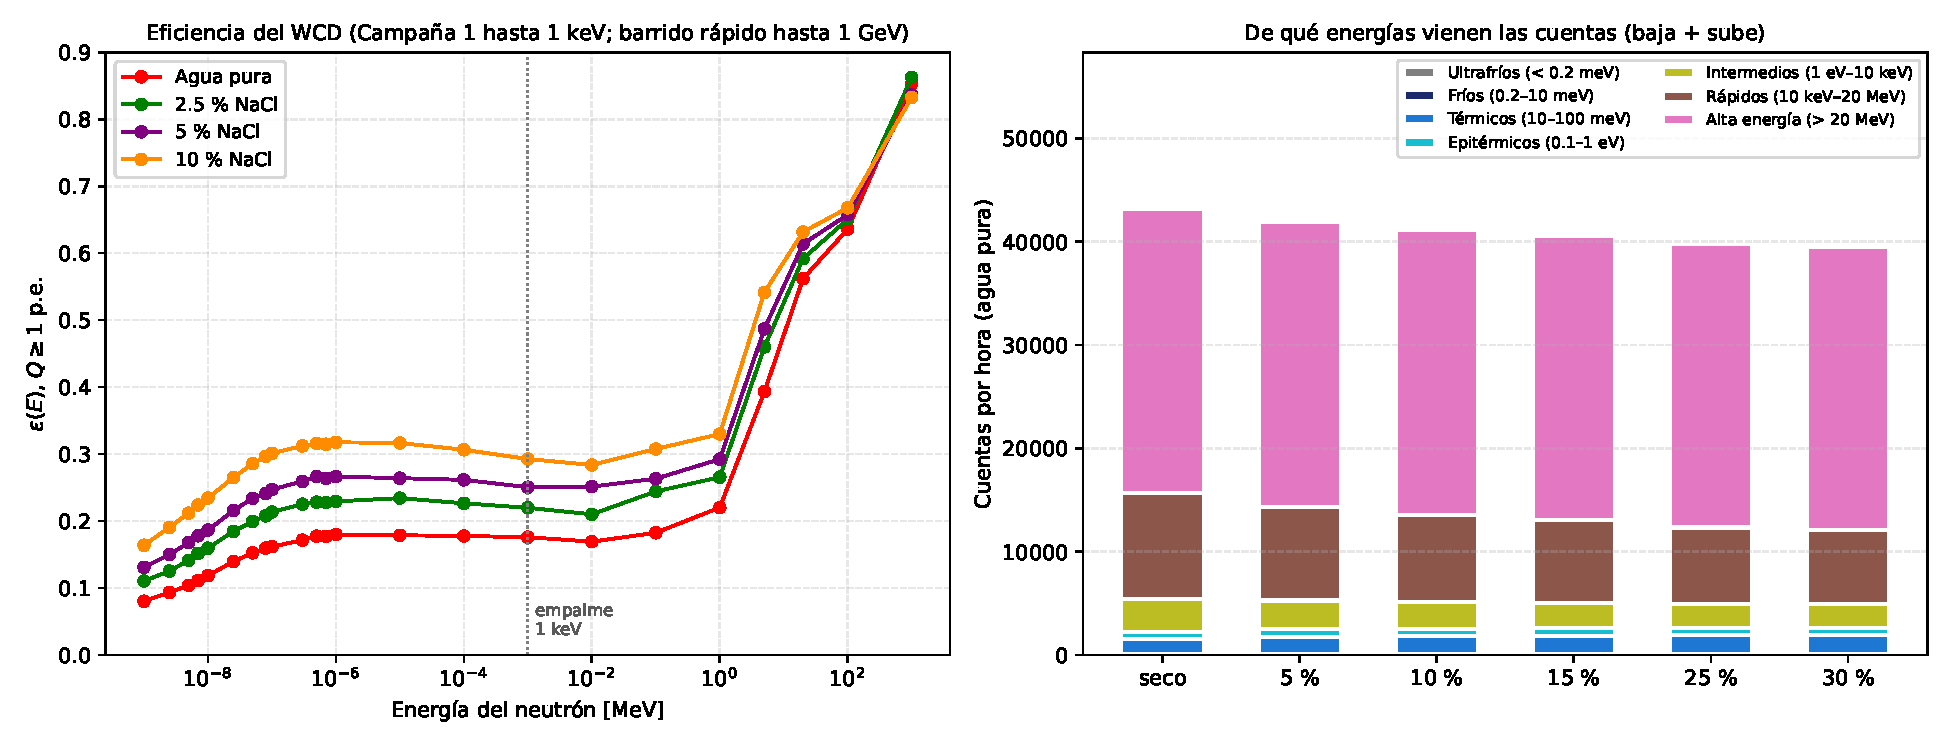
\includegraphics[width=\linewidth]{fig10_cuentas_por_banda.pdf}
\caption{Izquierda: eficiencia $\varepsilon(E)$ con $Q\geq1$~p.e.\ de 1~meV a 1~GeV. Derecha: cuentas por hora del WCD
con agua pura, separadas por la energía del neutrón que las produce (flujo que baja más el que sube).}\label{fig:band}
\end{figure}

\subsection{Coeficientes de captura, reflexión y transmisión}\label{sec:cap}
La captura de los neutrones en el agua es la señal que el WCD aprovecha (la cascada gamma de la captura, sobre todo la
del Cl con NaCl). Se usan la definición y el formato de la Tabla~4.8 y las Tablas~C.3--C.5 de la tesis: cada neutrón
incidente se clasifica por la última frontera del volumen activo ($|x|, |y| \le 48$~cm, $0 \le z \le 133$~cm) que
atraviesa, en captura ($\eta_{\rm Cap}$, su historia termina en \texttt{nCapture}), reflexión ($\eta_{\rm Refle}$,
sale por la cara superior), transmisión ($\eta_{\rm Trans}$, sale por el fondo o las paredes laterales) y otros
destinos ($\eta_{\rm Otros}$, no ingresa al volumen activo o su historia termina en una interacción inelástica). Solo
cuenta el neutrón incidente; la incertidumbre es la binomial, $\sqrt{\eta(1-\eta)/N}$ (1$\sigma$).
\begin{itemize}
\item De 1~meV a 1~keV: la Campaña~1, $10^5$ neutrones monocromáticos verticales por energía (los números de la
tesis, de \archivo{balance_caras_tanque.py}).
\item De 10~keV a 1~GeV: el barrido rápido (1\,000 a 10\,000 neutrones por energía), con la misma clasificación
(\archivo{balance_rapidos.py}).
\end{itemize}
\ifbalancerapido\aviso{\textbf{Empalme en 1~keV.} El barrido repite la energía de 1~keV (puntos huecos en las figuras y filas
bajo la línea en las tablas). La captura coincide con la Campaña~1 (34.08 frente a 33.77~\% en agua pura; 38.07 frente a 37.57~\%,
41.49 frente a 40.93~\% y 46.00 frente a 45.41~\% con 2.5, 5 y 10~\% NaCl) y la ganancia relativa también (1.117,
1.217 y 1.350 frente a 1.112, 1.212 y 1.345), pero la reflexión es
4 puntos menor (60.57 frente a 64.56~\%), la transmisión 0.4 puntos mayor (0.48 frente a 0.04~\%) y los otros destinos
3 puntos mayores (4.87 frente a 1.63~\%; casi todos neutrones que no llegan a entrar: 4.2 frente a 0.45~\%). Lo más
probable es que la diferencia venga de la inyección del barrido: desde $z = 200$~cm, con 67~cm de aire sobre la tapa, y
uniforme en un círculo de 40~cm de radio, de modo que más neutrones se dispersan en el aire antes de llegar y más
entran cerca de la pared lateral. Por eso los valores absolutos de reflexión, transmisión y otros destinos del barrido
deben compararse entre sí, y no punto a punto con los de la Campaña~1.}\else\aviso{Pendiente: el balance del barrido rápido (10~keV--1~GeV). Las tablas y la figura llegan por
ahora hasta 1~keV. Hace falta leer \archivo{pasos-neutrones.tsv} de las corridas del barrido, que están en el disco
ADATA; con el disco conectado, \archivo{scripts/actualizar_informe.sh} lo calcula y completa esta sección. La columna
``capturas en el agua'' del barrido (tabla~\ref{tab:eff}) no sirve para esto: cuenta los eventos con al menos una
captura de \emph{cualquier} neutrón, incluidos los secundarios, y no el destino del neutrón incidente.}\fi

\begin{figure}[H]\centering
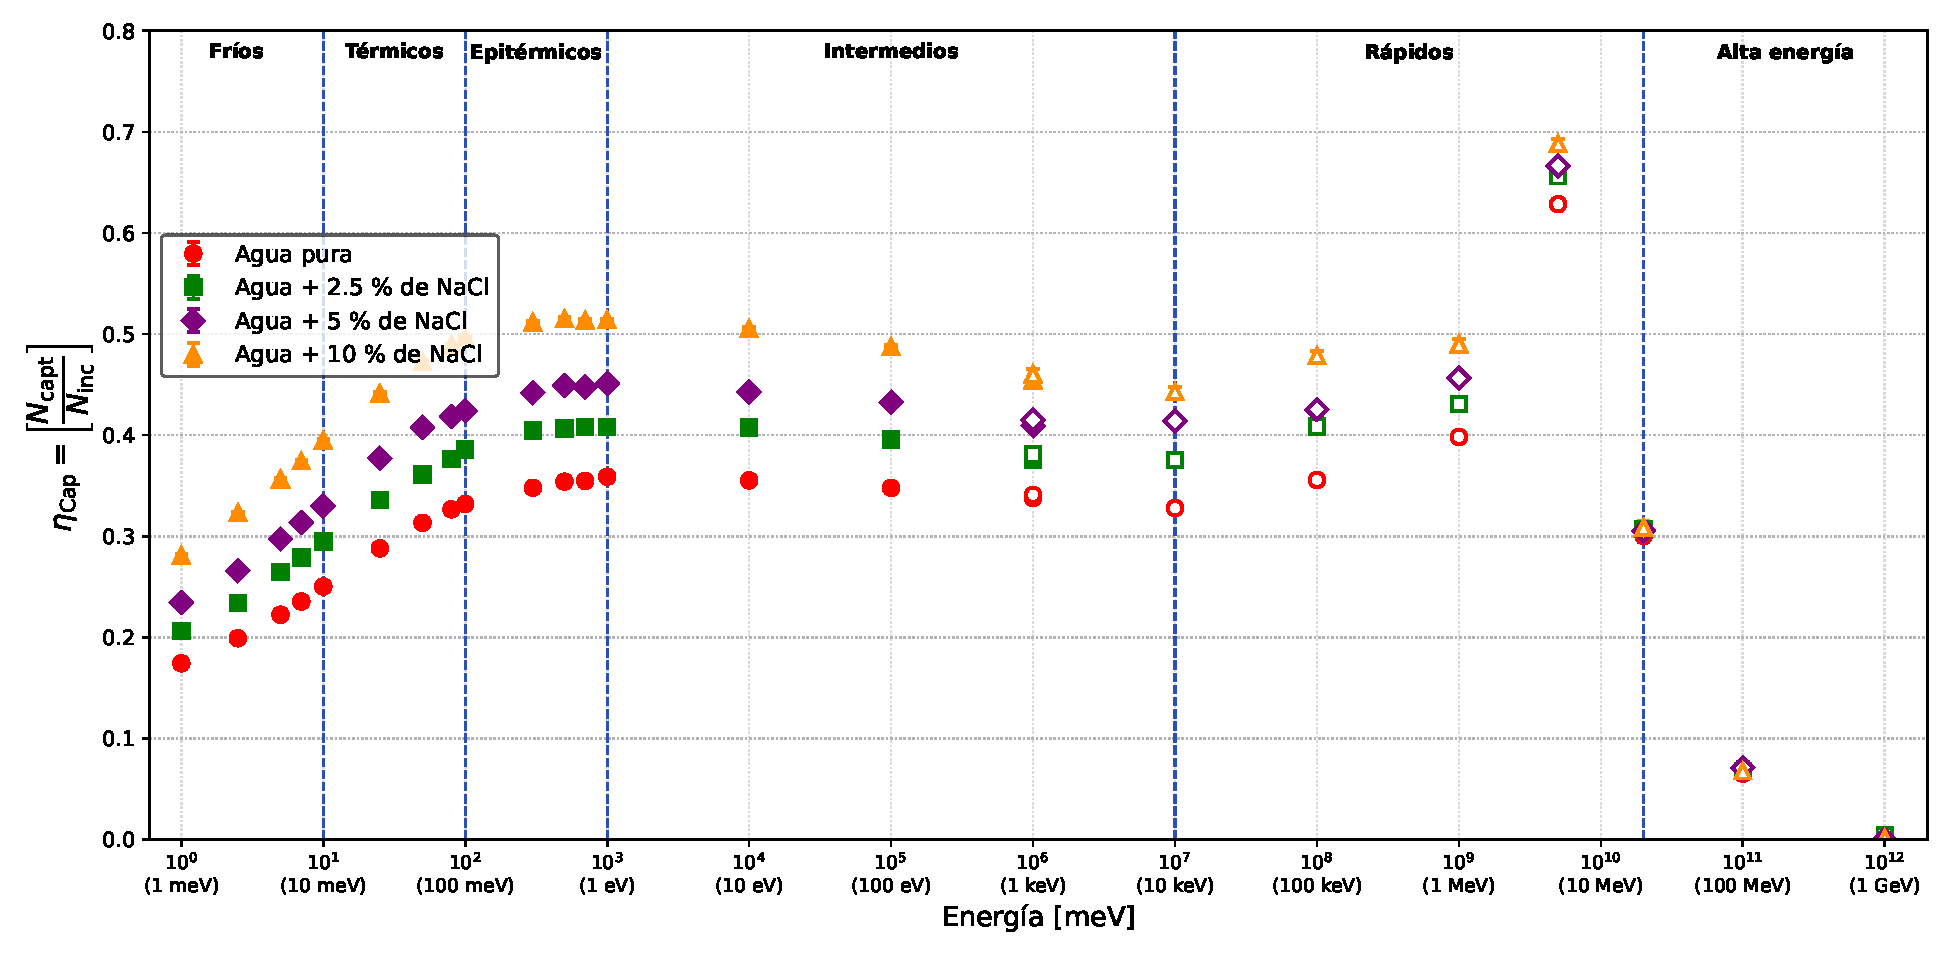
\includegraphics[width=\linewidth]{fig15_captura_wcd.pdf}
\caption{Coeficiente de captura de neutrones $\eta_{\rm Cap} = N_{\rm capt}/N_{\rm inc}$ en función de la energía
inicial, con las regiones de la tabla~\ref{tab:clasif}. Neutrones monocromáticos incidentes verticalmente sobre el
tanque. Se comparan agua pura (rojo), agua con 2.5~\% de NaCl (verde), agua con 5~\% de NaCl (violeta) y agua con
10~\% de NaCl (naranja). Símbolos llenos: Campaña~1 (hasta 1~keV); huecos: barrido rápido (1~keV a 1~GeV). Las
barras de error representan la incertidumbre estadística estándar (1$\sigma$).}\label{fig:cap}
\end{figure}

\begin{table}[H]
	\centering
	\caption{Coeficiente de captura $\eta_{\rm Cap}$ (\%) por energía y medio, agrupado por región
		(tabla~\ref{tab:clasif}), con su incertidumbre estadística (1$\sigma$).}\label{tab:cap_wcd}	
	\footnotesize\setlength\tabcolsep{4pt}
\tabla{captura_wcd}
\end{table}

\paragraph{De 1~keV a 1~GeV.} Por encima de los intermedios el destino del neutrón incidente cambia por completo
(figuras~\ref{fig:cap}, \ref{fig:refl} y~\ref{fig:transotr}):
\begin{itemize}
\item \textbf{Rápidos.} $\eta_{\rm Cap}$ sube de 32.8~\% (10~keV) a 39.8~\% (1~MeV) y llega al máximo en 5~MeV:
62.8~\% en agua pura, 65.6, 66.6 y 68.8~\% con 2.5, 5 y 10~\% NaCl. Un neutrón de unos MeV penetra hasta el centro del tanque antes de
frenarse y tiene menos probabilidad de volver a salir por la tapa: la reflexión baja de 62.7 a 28.1~\% (agua pura)
entre 10~keV y 5~MeV, y la transmisión sube a 4~\%.
\item \textbf{Alta energía.} Desde 20~MeV el neutrón incidente casi no se captura: $\eta_{\rm Cap}$ = 30~\% en
20~MeV, 6.5--7~\% en 100~MeV y 0--0.4~\% en 1~GeV. Domina $\eta_{\rm Otros}$ (53~\% en 20~MeV, 69--70~\% en 100~MeV y
79--81~\% en 1~GeV), es decir, historias que terminan en una interacción inelástica que destruye el neutrón y crea
otros, y la transmisión (20--24~\% en 100~MeV y 1~GeV: el neutrón atraviesa el tanque). La reflexión cae por debajo
del 2~\%. Los neutrones secundarios de esas reacciones sí se capturan en el agua, pero no cuentan en $\eta_{\rm Cap}$,
que sigue solo al neutrón incidente; por eso la eficiencia de señal del WCD (figura~\ref{fig:band}) sigue creciendo
con la energía aunque $\eta_{\rm Cap}$ caiga.
\item \textbf{Efecto del NaCl.} La ganancia relativa entre 1 y 100~keV es de 1.11--1.15 con 2.5~\%, 1.20--1.26 con
5~\% y 1.35 con 10~\% NaCl; en 1~MeV, 1.08, 1.15 y 1.23; en 5~MeV, 1.04, 1.06 y 1.10, y en 20~MeV, 1.02--1.03 en los
tres (figura~\ref{fig:caprel}): el NaCl actúa sobre el neutrón ya frenado, y su efecto se pierde
cuando el neutrón incidente deja de frenarse en el agua. En 100~MeV los cocientes tienen errores de $\pm$0.12.
\end{itemize}

\paragraph{Comparación con Sidelnik et al.} Sidelnik et al.~\cite{Sidelnik2020} encuentran, con 150\,000
neutrones de 500~MeV, una probabilidad de captura de 25.18~\% en agua pura y 26.73~\% con 2.5~\% de NaCl (su tabla~2),
mucho mayor que el $\eta_{\rm Cap}$ de 0.3--7~\% de la tabla~\ref{tab:cap_wcd} entre 100~MeV y 1~GeV. No es una
contradicción: son definiciones distintas. Sidelnik divide las capturas en el agua por \emph{todas} las trazas de
neutrones del evento (el incidente más los que crea la cascada), mientras que $\eta_{\rm Cap}$ sigue solo al neutrón
incidente, que a esas energías casi siempre se destruye en su primera interacción inelástica. La
tabla~\ref{tab:capdef} compara cuatro maneras de contar la captura en el barrido. Con la definición de Sidelnik, el
barrido da 27.4~\% en 100~MeV y 24.9~\% en 1~GeV en agua pura, en el intervalo de su 25.18~\% en 500~MeV, y 27.3 y 25.5~\% con 2.5~\% de NaCl, alrededor de su 26.73~\% (con 5 y
10~\%, 28.3/26.6 y 28.8/28.5~\%); la réplica de
su corrida en MEIGA (sección~4.1.1 de la tesis) dio 24.08~\% en agua pura y 24.67~\% con 2.5~\% de NaCl. Por debajo de
5~MeV hay una sola traza por evento y las cuatro definiciones coinciden (la pequeña diferencia con $\eta_{\rm Cap}$ son
las capturas fuera del agua, que $\eta_{\rm Cap}$ incluye).

\begin{table}[H]
	\centering
	\caption{Cuatro definiciones de la captura en el barrido rápido: $\eta_{\rm Cap}$ (destino del neutrón incidente,
		dentro o fuera del agua); capturas en el agua por traza de neutrón del evento (definición de Sidelnik et
		al.~\cite{Sidelnik2020}); capturas en el agua por neutrón incidente (puede superar el 100~\%); y fracción de eventos con
		al menos una captura en el agua. Se dan también las trazas de neutrones por neutrón incidente.}\label{tab:capdef}	
	\footnotesize\setlength\tabcolsep{3.5pt}
\tabla{capturas_definiciones}
\end{table}

\paragraph{Coeficiente de reflexión.} $\eta_{\rm Refle}(E_n)$ es la fracción de neutrones que ingresan al volumen
activo y lo abandonan por la cara superior, es decir, por la frontera de incidencia: la historia entra, se dispersa y
regresa. Cuantifica un destino final y no una ausencia de interacción.

\begin{figure}[H]\centering
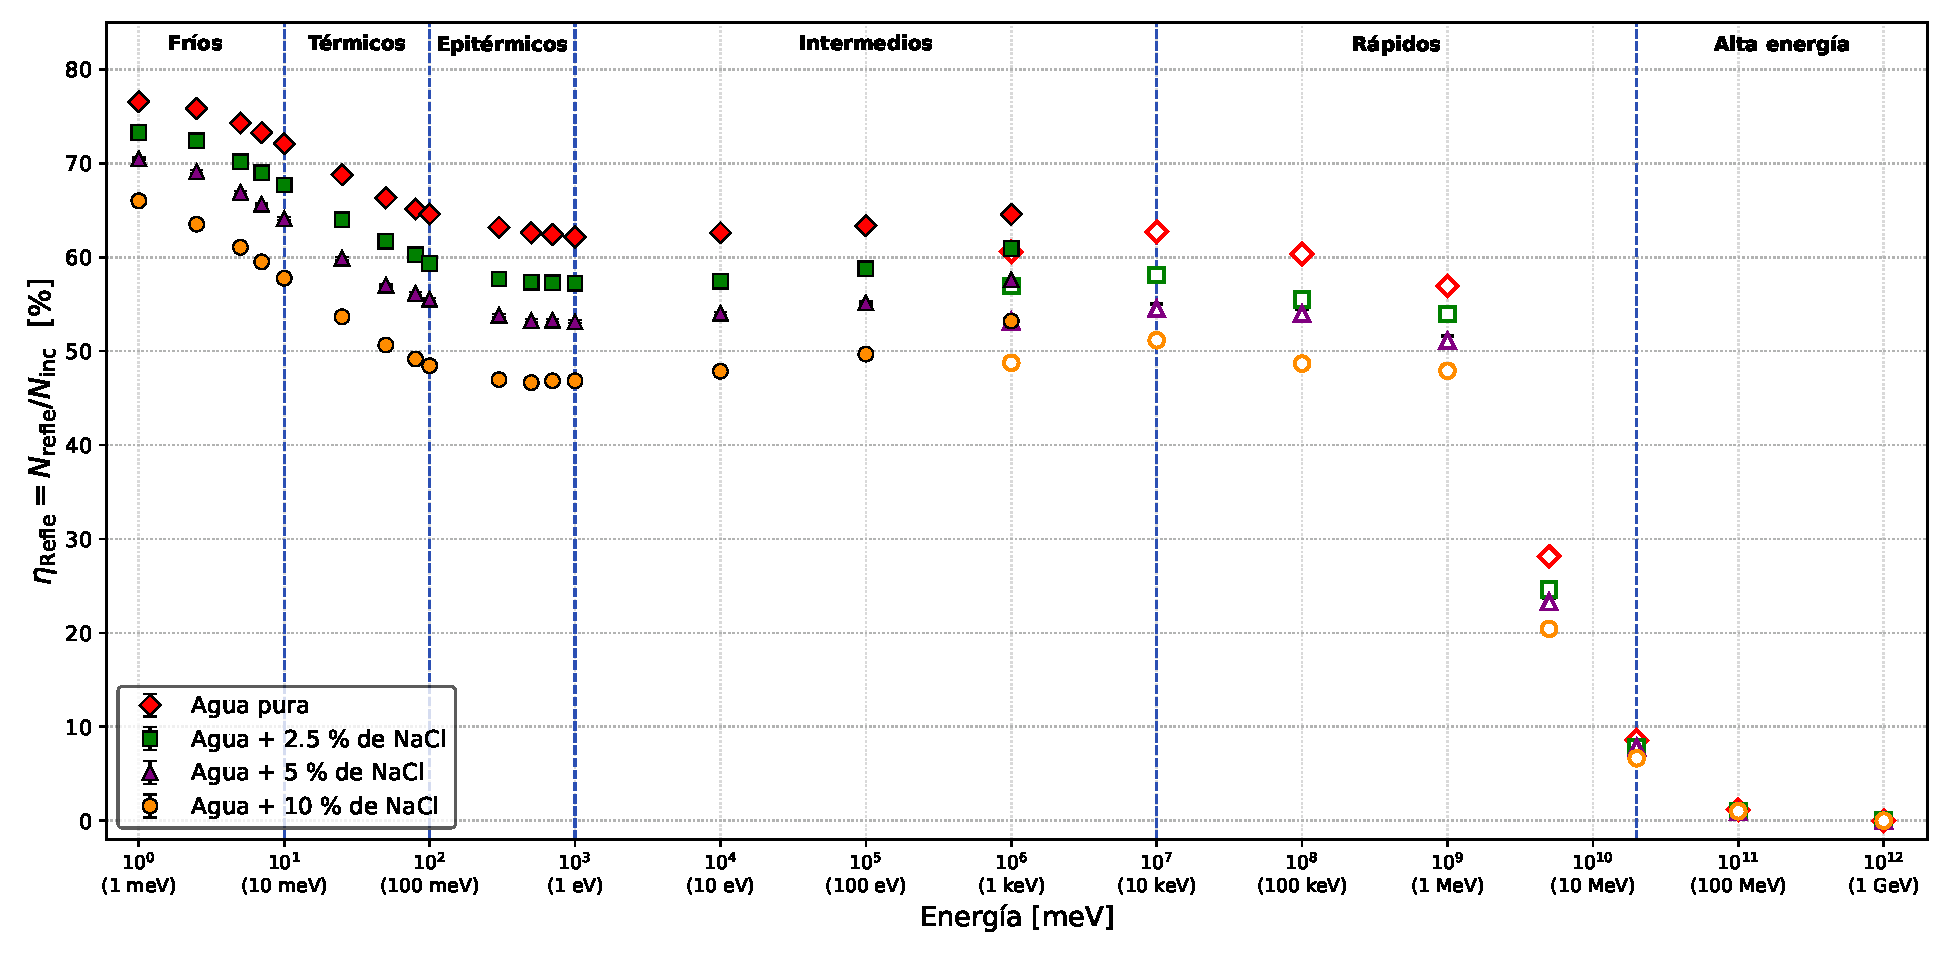
\includegraphics[width=\linewidth]{fig16_reflexion_wcd.pdf}
\caption{Coeficiente de reflexión de neutrones $\eta_{\rm Refle} = N_{\rm refle}/N_{\rm inc}$, definido como la
fracción de neutrones que abandonan el volumen activo por su cara superior, en función de la energía inicial, con las
regiones de la tabla~\ref{tab:clasif}, para agua pura y soluciones con 2.5, 5 y 10~\% de NaCl (esquema de la
figura~4.25 de la tesis). Símbolos llenos: Campaña~1; huecos: barrido rápido. Las barras de error representan la
incertidumbre estadística estándar (1$\sigma$).}\label{fig:refl}
\end{figure}

La reflexión es el destino dominante y sigue la tendencia opuesta a la captura. En agua pura, $\eta_{\rm Refle}$ baja de
$(76.569\pm0.134)$~\% en 1~meV a $(62.168\pm0.153)$~\% en 1~eV y vuelve a subir hasta $(64.560\pm0.151)$~\% en 1~keV;
el mínimo amplio entre 300~meV y 10~eV (epitérmicos y comienzo de los intermedios) coincide con el máximo de la captura.
El NaCl reduce la fracción reflejada en todo el intervalo: en 1~meV, de $(76.569\pm0.134)$~\% en agua pura a
$(73.295\pm0.140)$, $(70.466\pm0.144)$ y $(66.012\pm0.150)$~\% con 2.5, 5 y 10~\% de NaCl; en 1~eV, de
$(62.168\pm0.153)$~\% a $(57.236\pm0.156)$, $(53.127\pm0.158)$ y $(46.843\pm0.158)$~\%. Esa reducción es la
otra cara del aumento de la captura: las historias se redistribuyen entre los destinos posibles, cuya suma es 1.

\paragraph{Coeficientes de transmisión y de otros destinos.} $\eta_{\rm Trans}(E_n)$ es la fracción de neutrones que
ingresan al medio detector, no son capturados y lo abandonan por el fondo o por las paredes laterales. En el intervalo de
la Campaña~1 este canal es prácticamente despreciable (figura~\ref{fig:transotr}a): en todas las energías y medios se
mantiene entre 0.02 y 0.06~\%, con incertidumbres de $\sim$0.006 puntos porcentuales, sin una dependencia sistemática con
la energía ni con la concentración de NaCl. Los neutrones de baja energía que ingresan por la tapa se moderan y se
capturan en los primeros centímetros del medio, de modo que muy pocos alcanzan el fondo o las paredes laterales,
situados a distancias mucho mayores que su recorrido típico.

$\eta_{\rm Otros}(E_n)$ (figura~\ref{fig:transotr}b) agrupa los neutrones que no llegan a ingresar al volumen activo y
aquellos cuya historia termina en una interacción inelástica. En agua pura baja de $(5.968\pm0.075)$~\% en 1~meV a
$(1.913\pm0.043)$~\% en 1~eV y $(1.626\pm0.040)$~\% en 1~keV. En 1~meV, 3.6 puntos corresponden a neutrones que no
ingresan al volumen activo y 2.4 a interacciones inelásticas, casi todas fuera del medio detector (2\,272 de 2\,379).
Depende muy poco de la concentración de NaCl, porque son procesos que ocurren sobre todo antes de que el neutrón alcance
el medio.

\begin{figure}[H]\centering
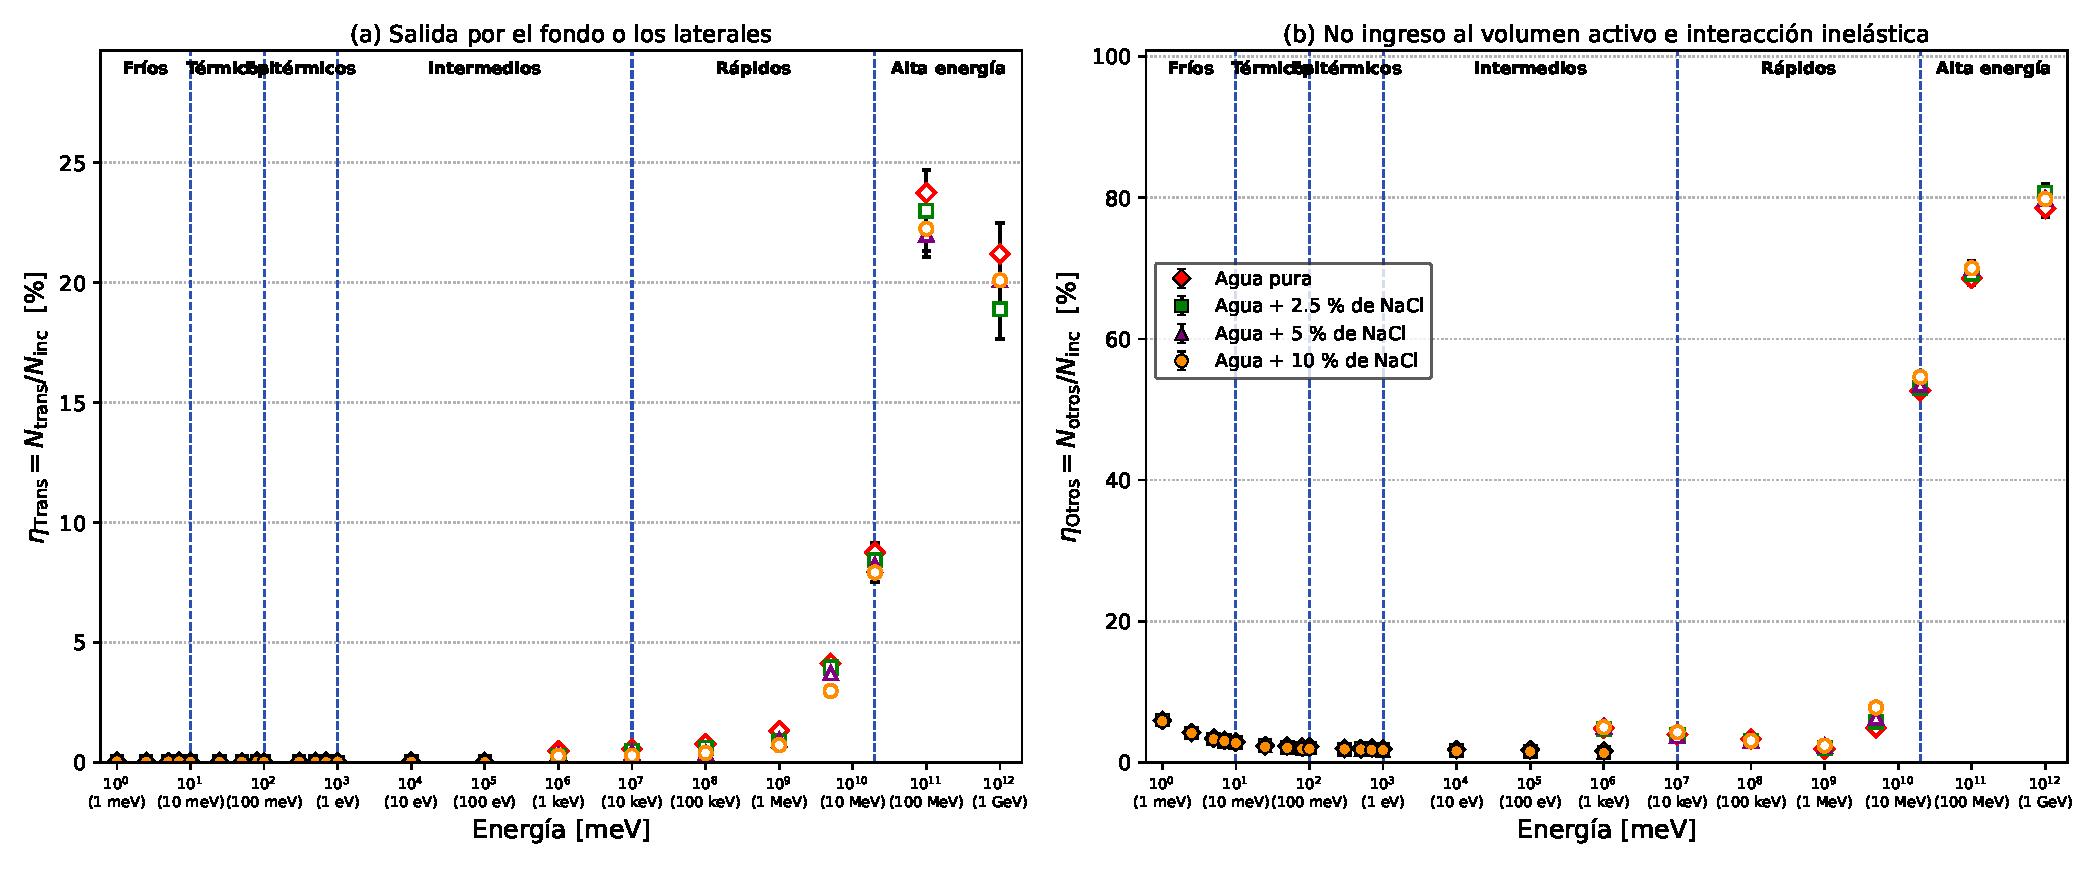
\includegraphics[width=\linewidth]{fig17_transmision_otros_wcd.pdf}
\caption{(a) Coeficiente de transmisión de neutrones $\eta_{\rm Trans} = N_{\rm trans}/N_{\rm inc}$ (salida por el
fondo o las paredes laterales del volumen activo) y (b) coeficiente de otros destinos
$\eta_{\rm Otros} = N_{\rm otros}/N_{\rm inc}$ (neutrones que no ingresan al volumen activo o cuya historia termina en
una interacción inelástica), en función de la energía inicial, con las regiones de la tabla~\ref{tab:clasif}, para agua
pura y soluciones con 2.5, 5 y 10~\% de NaCl (esquema de la figura~4.26 de la tesis). Símbolos llenos: Campaña~1;
huecos: barrido rápido. Las barras de error representan la incertidumbre estadística estándar (1$\sigma$).}\label{fig:transotr}
\end{figure}

\paragraph{Eficiencia relativa de captura.} La figura~\ref{fig:caprel} muestra la captura relativa en el volumen del
detector con dopante frente al agua pura, $\eta_{\rm capt,rel} = \eta_{\rm Cap}({\rm NaCl})/\eta_{\rm Cap}({\rm agua})$:
mide la ganancia que introduce el NaCl. La incertidumbre combina la de las dos corridas, que son independientes
(tabla~\ref{tab:caprel}).

\begin{figure}[H]\centering
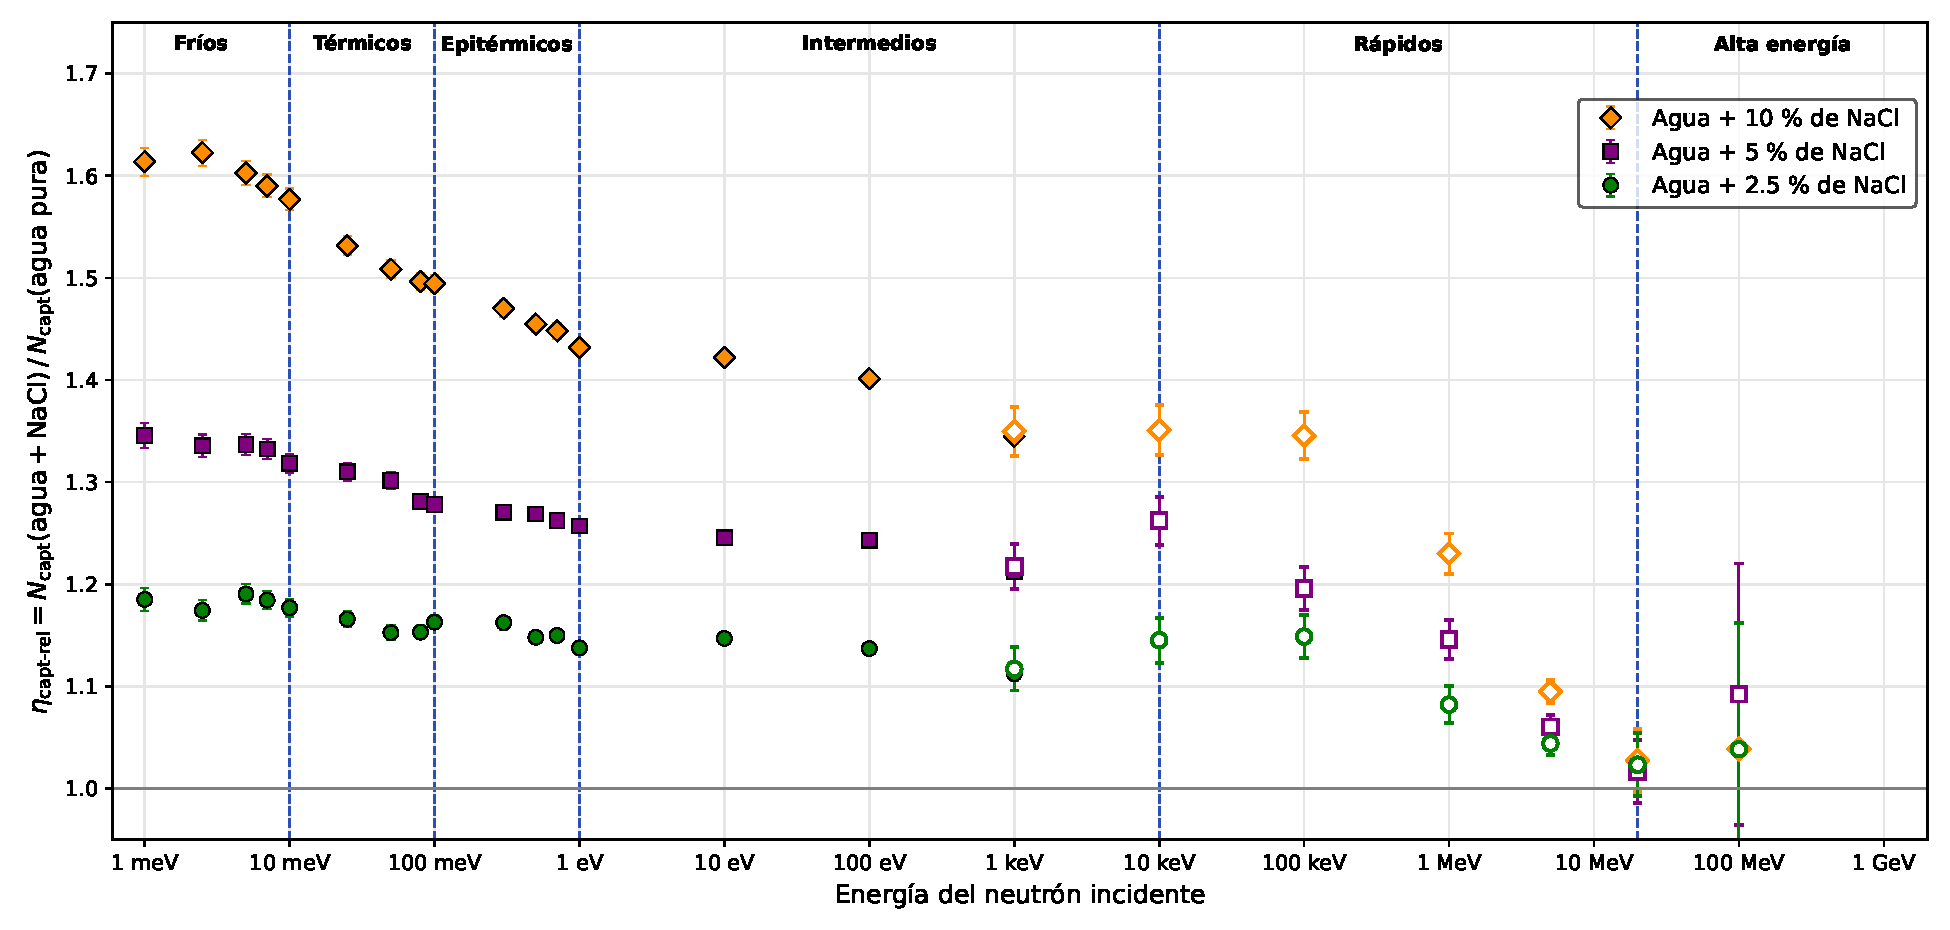
\includegraphics[width=\linewidth]{fig18_captura_relativa_wcd.pdf}
\caption{Ganancia relativa de captura, $\eta_{\rm capt,rel} = \eta_{\rm capt}({\rm NaCl})/\eta_{\rm capt}({\rm agua})$,
con las regiones de la tabla~\ref{tab:clasif} (esquema de la figura~4.27 de la tesis). Los valores superiores a la
unidad cuantifican el incremento respecto al agua pura. La separación entre 5 y 10~\% permanece visible y no sustenta,
por sí sola, una saturación. Símbolos llenos: Campaña~1; huecos: barrido rápido (en 1~GeV hay menos de 20 capturas del
neutrón incidente y no se calcula el cociente).}\label{fig:caprel}
\end{figure}

Cada curva se mantiene por encima de la unidad en $1~{\rm meV}\le E_n\le 1~{\rm keV}$: hay ganancia de captura para las
tres concentraciones. La ganancia es mayor en los fríos (1.61, 1.35 y 1.19 en 1~meV para 10, 5 y 2.5~\% de NaCl) y
disminuye hacia 1~keV, donde las razones son 1.34, 1.21 y 1.11. La tendencia es compatible con la elevada absorción
térmica del $^{35}$Cl y con la competencia entre captura y escape, pero la razón macroscópica no es una medida directa
de una ley $1/v$: también contiene moderación, composición, geometría y selección de historias. El resultado coincide
cualitativamente con el aumento de la captura con la salinidad que reportan Sidelnik et al.~\cite{Sidelnik2020},
aunque aquel estudio usó neutrones de 500~MeV y otra geometría de incidencia. La separación persistente entre 5 y 10~\%
muestra que los datos de captura no justifican describir la respuesta como saturada por encima de 5~\%; la
optimización exige incorporar la respuesta óptica y criterios experimentales.

\begin{table}[H]
	\centering
	\caption{Ganancia relativa de captura $\eta_{\rm capt,rel}$ por energía y concentración de NaCl, agrupada por región
		(tabla~\ref{tab:clasif}), con su incertidumbre estadística (1$\sigma$).}\label{tab:caprel}
		\footnotesize
\tabla{captura_relativa}
\end{table}

\newcommand{\pieBalance}[1]{Coeficientes de captura $\eta_{\rm Cap}$, reflexión $\eta_{\rm Refle}$ (salida por la
cara superior del tanque), transmisión $\eta_{\rm Trans}$ (salida por el fondo o las paredes laterales) y otros
destinos $\eta_{\rm Otros}$ (neutrones que no ingresan al volumen activo o cuya historia termina en una interacción
inelástica) para #1. La clasificación se basa en la última frontera del volumen activo atravesada por cada neutrón.
Hasta 1~keV, $10^5$ neutrones monocromáticos por energía (Campaña~1); bajo la línea, el barrido rápido (de 1~keV a
1~GeV; 10\,000 neutrones hasta 5~MeV, 5\,000 en 20~MeV, 2\,000 en 100~MeV y 1\,000 en 1~GeV). Los
coeficientes y sus incertidumbres estadísticas estándar (1$\sigma$) se expresan en porcentaje.}
\begin{table}[H]
	\centering
\caption{\pieBalance{agua pura}}\label{tab:bal_pura}	
	\small
\tabla{balance_agua_pura}
\end{table}
\begin{table}[H]
	\centering
	\caption{\pieBalance{agua con 2.5~\% de NaCl}}\label{tab:bal_25}	
	\small
\tabla{balance_nacl25}

\end{table}
\begin{table}[H]
	\centering
\caption{\pieBalance{agua con 5~\% de NaCl}}\label{tab:bal_5}	
	\small
\tabla{balance_nacl5}
\end{table}
\begin{table}[H]
	\centering
\caption{\pieBalance{agua con 10~\% de NaCl}}\label{tab:bal_10}
	\small
\tabla{balance_nacl10}
\end{table}

\begin{itemize}
\item \textbf{Fríos y térmicos:} $\eta_{\rm Cap}$ crece con la energía, de 17.4~\% (1~meV) a 33.2~\% (100~meV) en agua
pura, y $\eta_{\rm Refle}$ baja de 76.6 a 64.6~\%: los neutrones más lentos se reflejan por la tapa antes de entrar a
fondo en el agua.
\item \textbf{Epitérmicos:} meseta de $\eta_{\rm Cap}\approx35$--36~\% en agua pura, 40--41~\% con 2.5~\%, 44--45~\%
con 5~\% y 51~\% con 10~\% NaCl.
\item \textbf{Intermedios:} $\eta_{\rm Cap}$ baja despacio hasta 1~keV (33.8~\% en agua pura; 37.6, 40.9 y 45.4~\% con
2.5, 5 y 10~\% NaCl) y
$\eta_{\rm Refle}$ vuelve a subir.
\item \textbf{Transmisión y otros:} $\eta_{\rm Trans}$ queda entre 0.02 y 0.06~\% en todo el intervalo de la
Campaña~1 y $\eta_{\rm Otros}$ baja de 6 a 1.4--1.6~\% (figura~\ref{fig:transotr}).
\item \textbf{NaCl:} la captura es 1.19, 1.35 y 1.61 veces la del agua pura en 1~meV con 2.5, 5 y 10~\% NaCl, y 1.14,
1.26 y 1.43 veces en 1~eV; lo que gana la captura lo pierde la reflexión.
\end{itemize}
La figura~\ref{fig:refl} muestra la reflexión con el mismo esquema.
\begin{itemize}
\item \textbf{Reflexión:} baja desde los fríos hasta un mínimo amplio en los epitérmicos (62~\% en agua pura; 57, 53 y
47~\% con 2.5, 5 y 10~\% NaCl) y vuelve a subir en los intermedios.
\end{itemize}

\subsection{Fotones Cherenkov y fotoelectrones de 1~keV a 1~GeV}\label{sec:luz}
Con las mismas corridas del barrido rápido se obtuvieron, por neutrón incidente, los fotones Cherenkov aceptados y los
fotoelectrones. MEIGA corre en modo \texttt{eFast}, que aplica la eficiencia cuántica del PMT al crear cada fotón óptico:
el registro de cada corrida (\archivo{ejecucion.log}) anota el inicio de cada traza separado por evento, y contando las de
fotones ópticos se obtienen los \emph{fotones aceptados} por la eficiencia cuántica, la magnitud de la fig.~6 de Sidelnik
et al.~\cite{Sidelnik2020}, no todos los creados. Los fotoelectrones salen de \archivo{Carga-total.txt}. En ningún evento la
carga supera a los fotones aceptados, y la fracción con $Q\geq1$ coincide con la eficiencia del barrido.

\begin{figure}[H]\centering
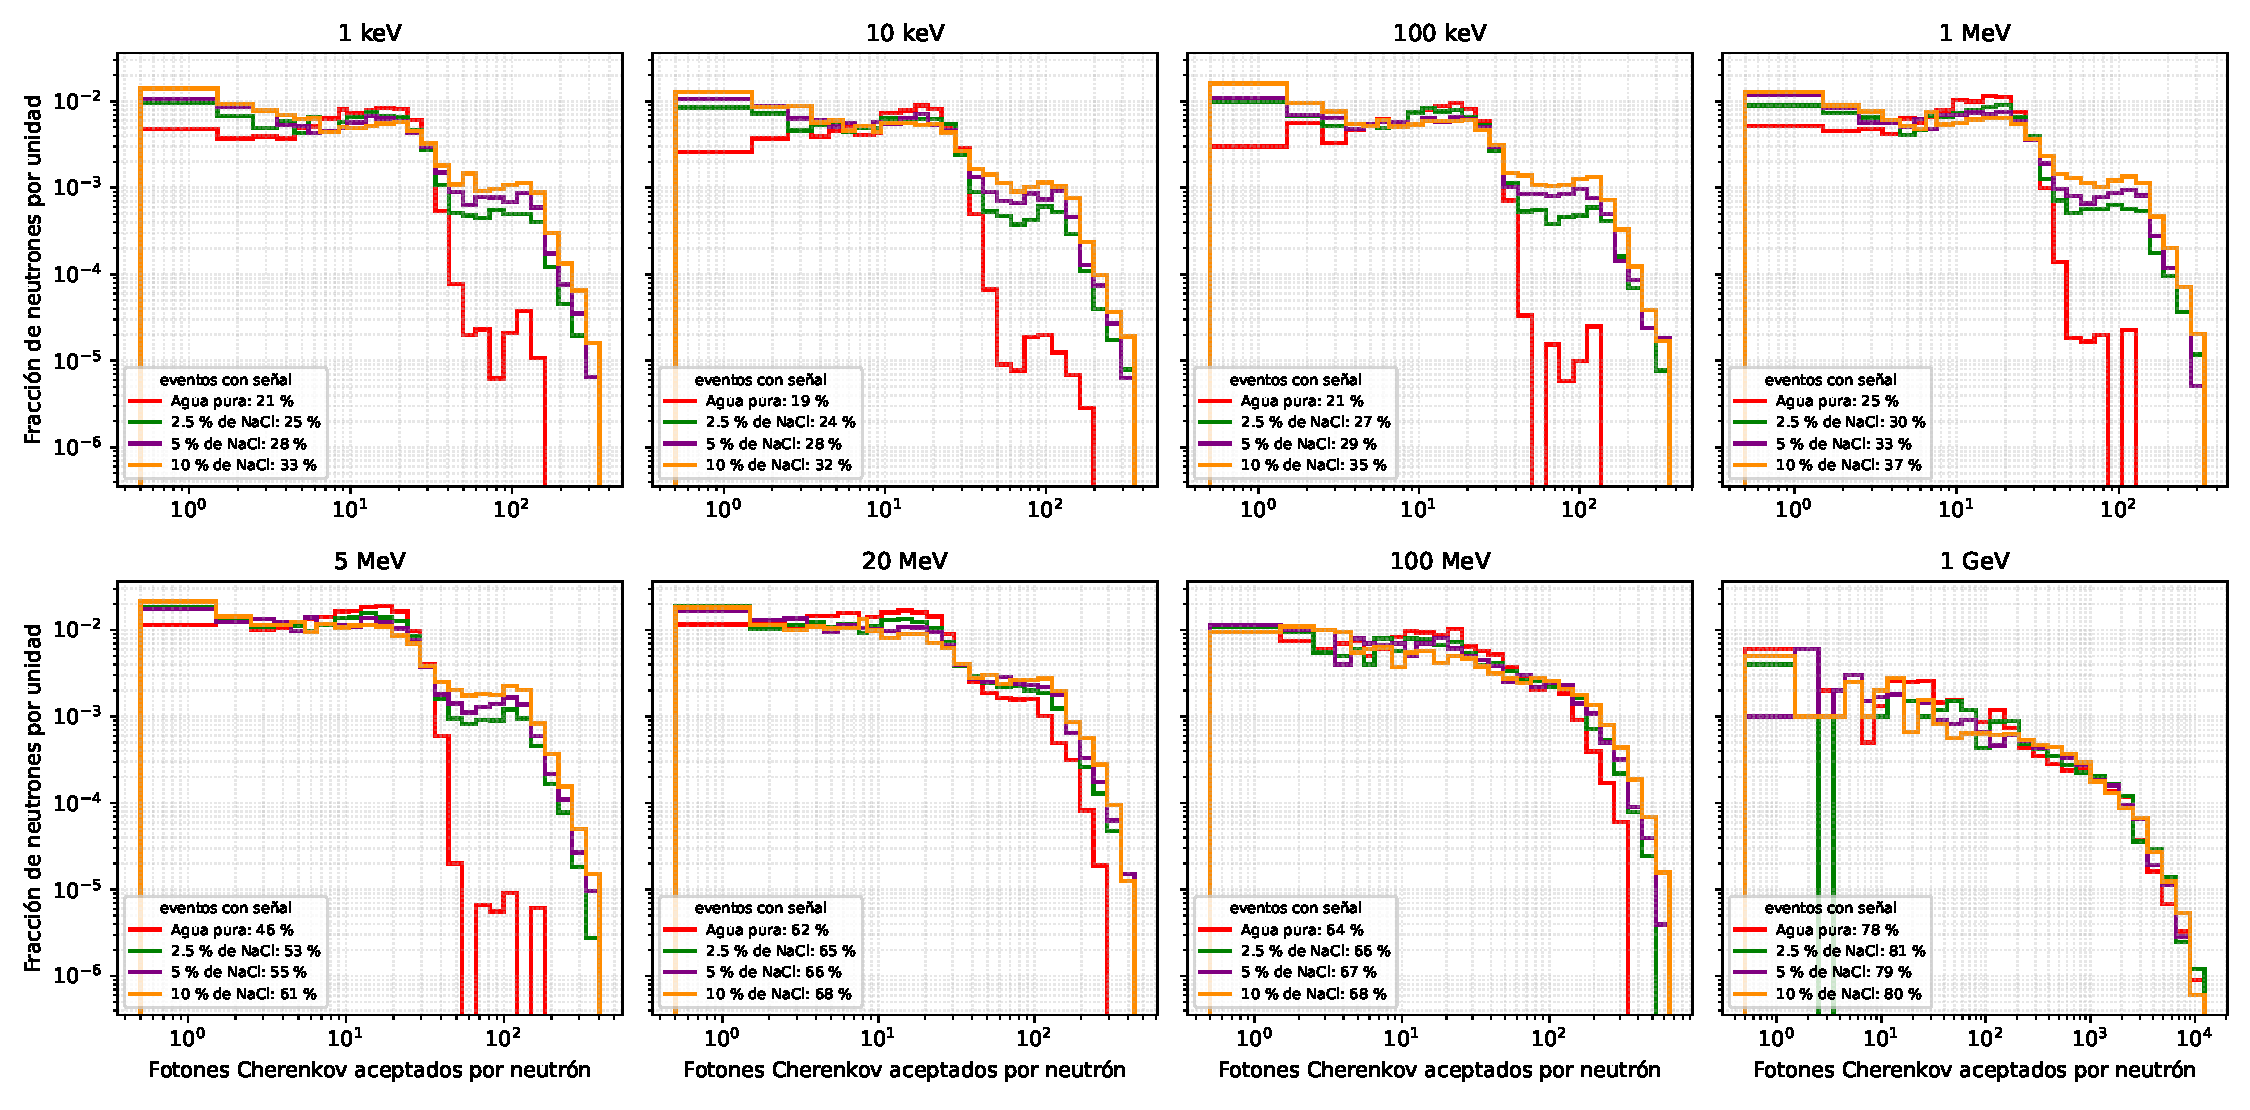
\includegraphics[width=\linewidth]{fig22_histogramas_fotones.pdf}
\caption{Histogramas de fotones Cherenkov aceptados por neutrón incidente, de 1~keV a 1~GeV, en los cuatro medios
(intervalos logarítmicos, normalizados al número de neutrones y al ancho del intervalo; no se dibujan los eventos sin
luz). En la leyenda, el porcentaje de neutrones con al menos un fotón aceptado.}\label{fig:histfot}
\end{figure}

\begin{figure}[H]\centering
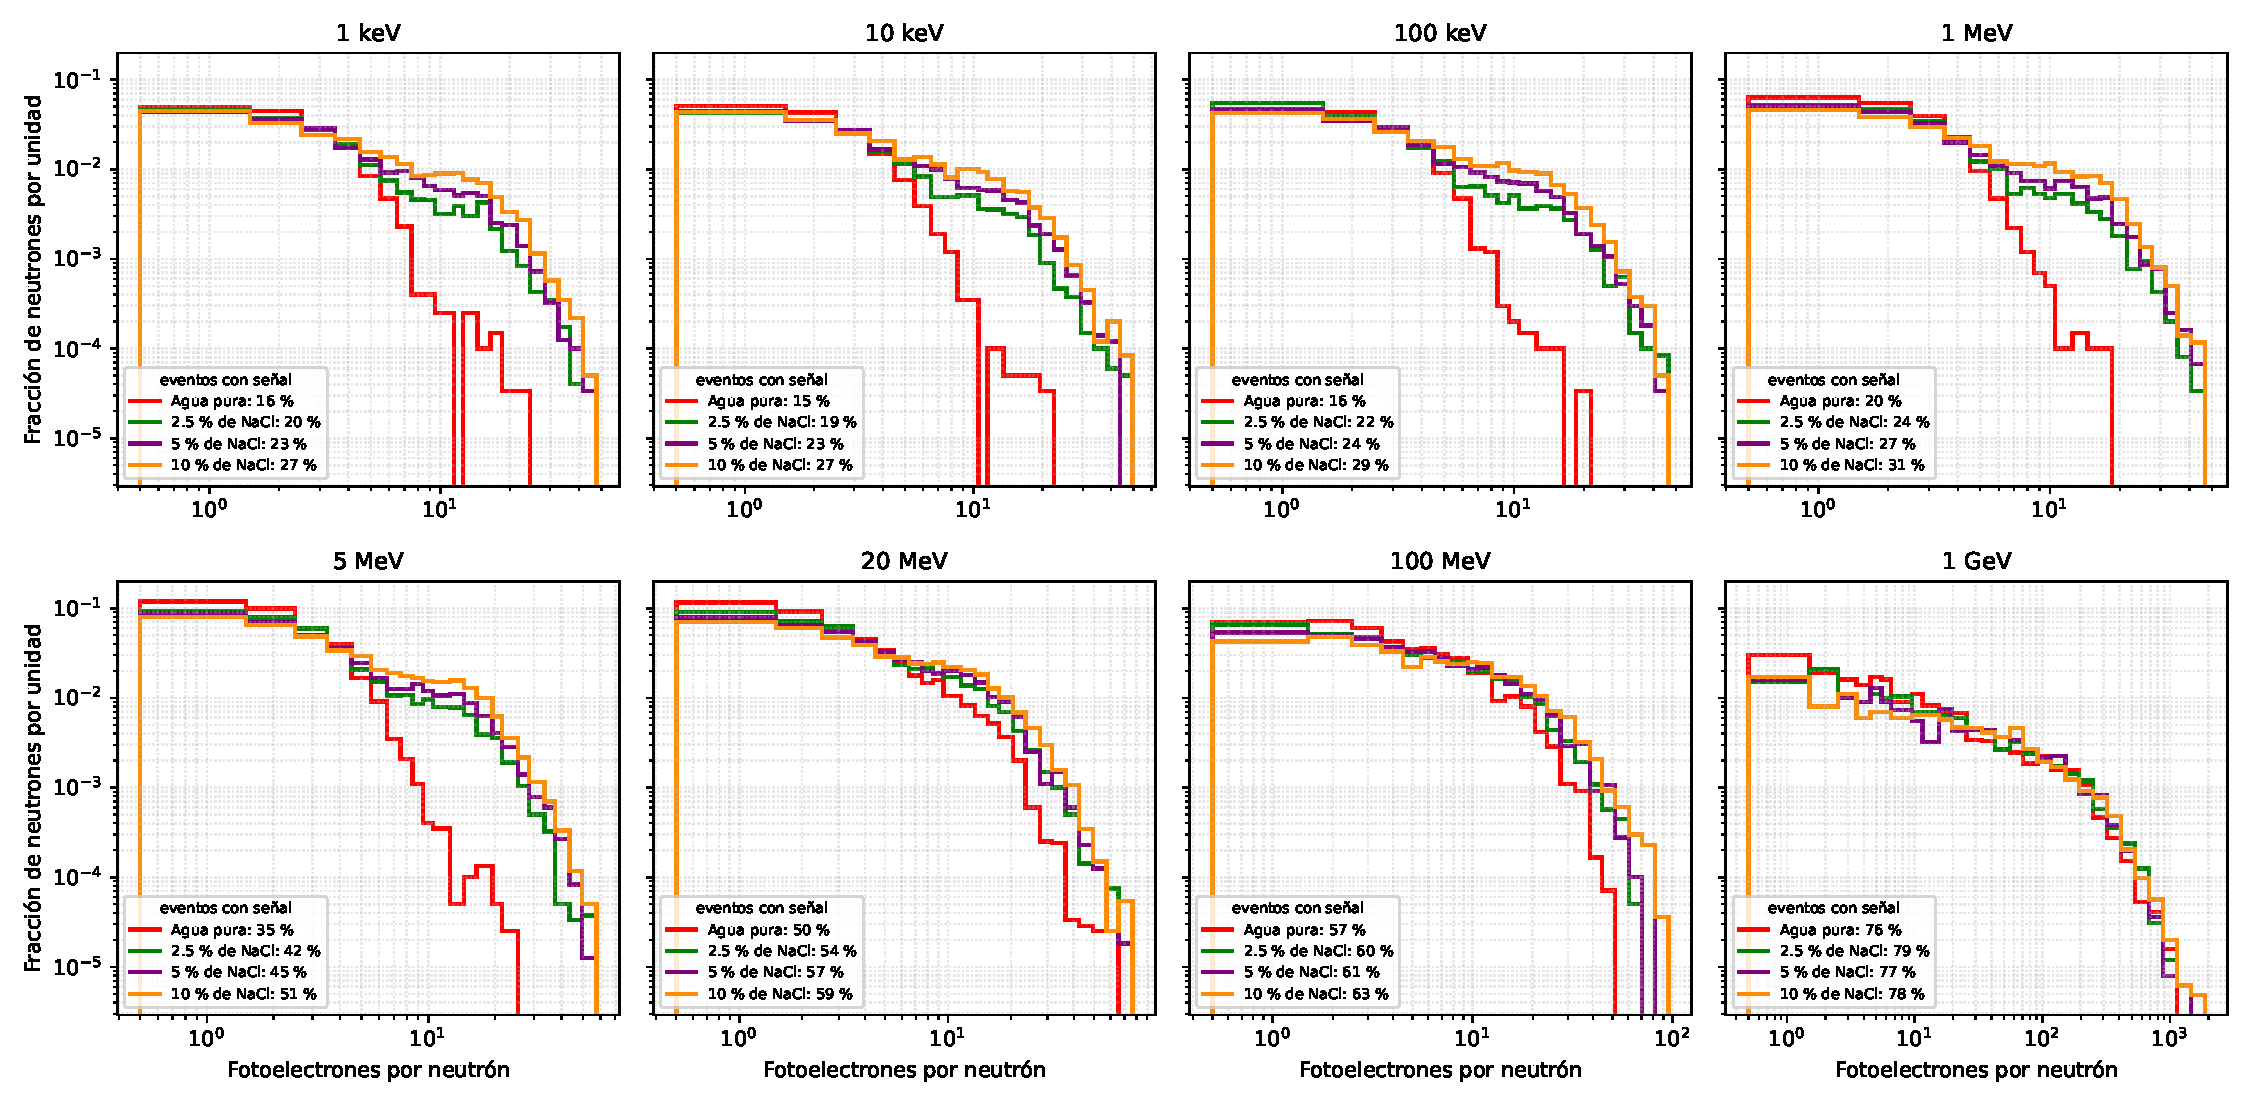
\includegraphics[width=\linewidth]{fig23_histogramas_fotoelectrones.pdf}
\caption{Histogramas de fotoelectrones por neutrón incidente, con el mismo esquema que la figura~\ref{fig:histfot}. En
la leyenda, el porcentaje de neutrones con $Q\geq1$~p.e.}\label{fig:histpe}
\end{figure}

\begin{figure}[H]\centering
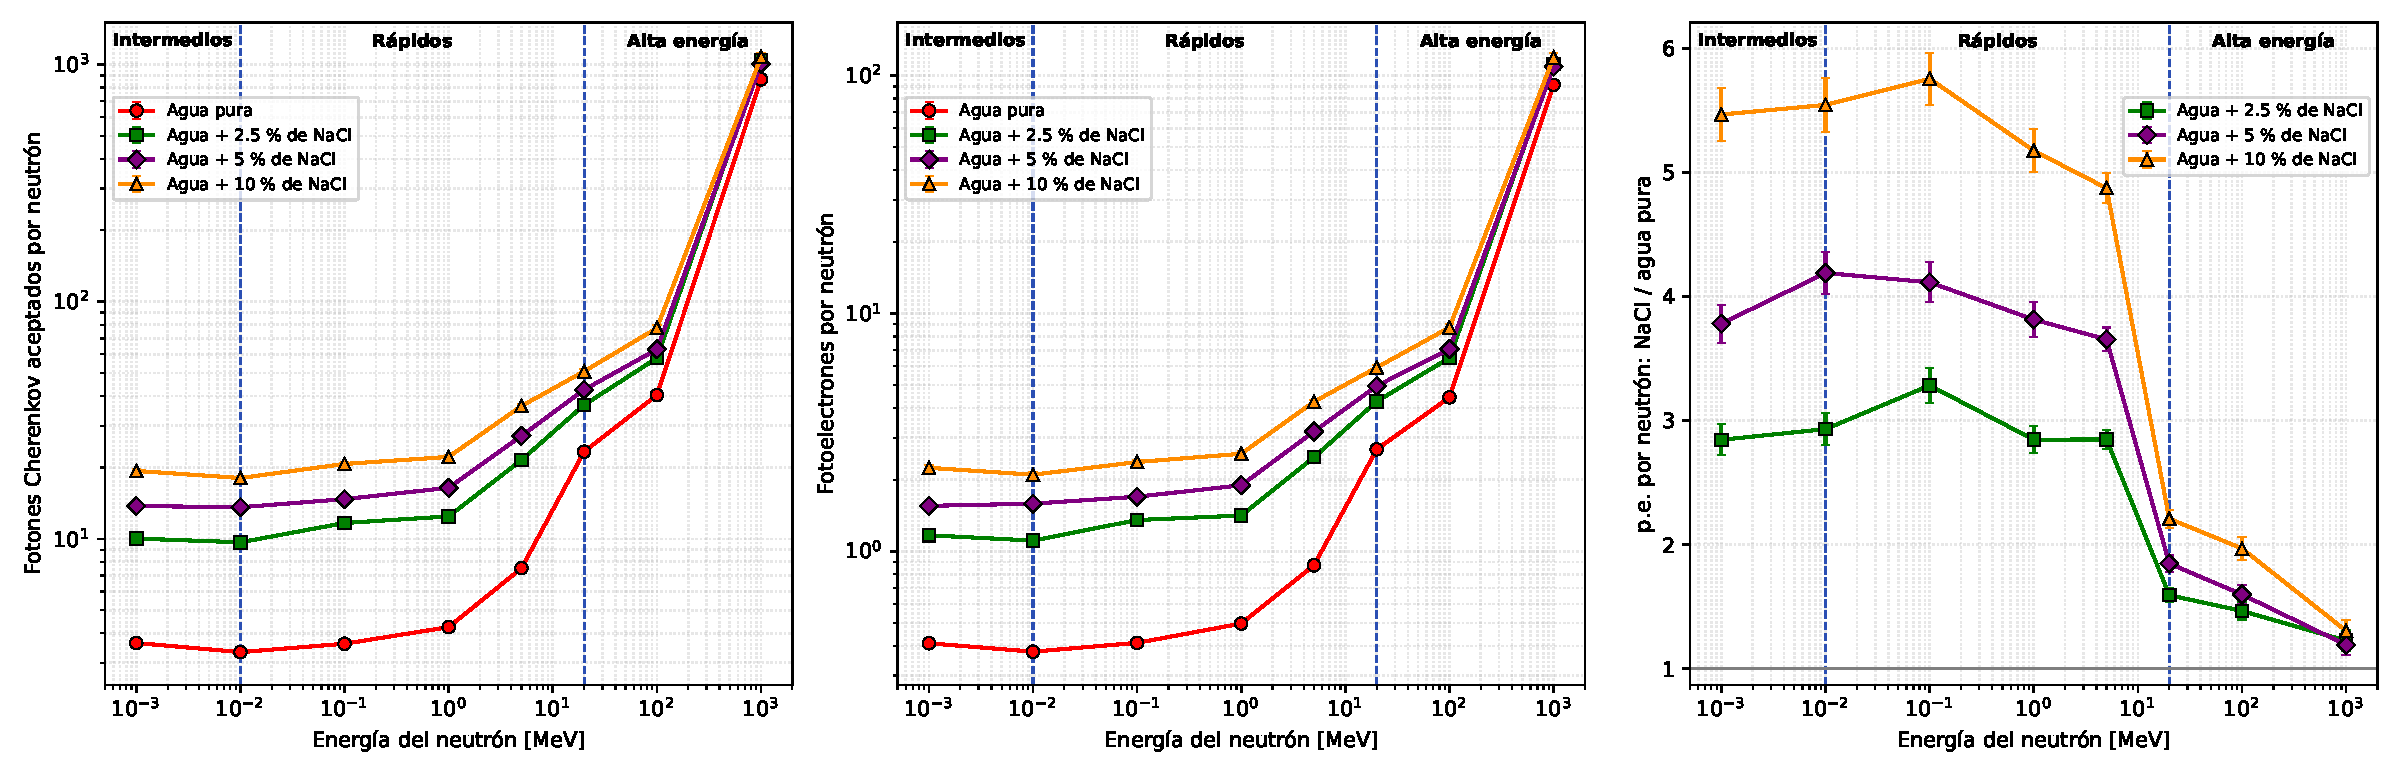
\includegraphics[width=\linewidth]{fig24_luz_vs_energia.pdf}
\caption{Fotones Cherenkov aceptados (izquierda) y fotoelectrones (centro) por neutrón incidente, en promedio, frente a la
energía, y cociente de los fotoelectrones con NaCl respecto del agua pura (derecha), con las regiones de la
tabla~\ref{tab:clasif}. Barras de error: error de la media (1$\sigma$).}\label{fig:luzE}
\end{figure}

\begin{table}[H]
	\centering
	\caption{Fotones Cherenkov aceptados y fotoelectrones por neutrón incidente (media sobre todos los neutrones, incluidos
		los que no dan luz) y fracción de fotones aceptados que llega al PMT como fotoelectrón.}\label{tab:luz}
	\footnotesize\setlength\tabcolsep{3pt}
\tablaancha{luz_barrido}

\end{table}

\begin{itemize}
\item \textbf{Forma de los histogramas.} En agua pura casi toda la luz de 1~keV a 5~MeV queda por debajo de
$\sim$30 fotones aceptados (99~\% de los neutrones con 32 o menos): es la luz de la captura en H (2.2~MeV). Con NaCl
aparece un segundo escalón de 40 a 300 fotones, de las cascadas de la captura en Cl ($\sim$8.6~MeV). Por encima de
20~MeV la luz de la propia interacción del neutrón rápido (protones de retroceso y cascadas inelásticas) borra esa
diferencia, y en 1~GeV los histogramas de los cuatro medios llegan a $10^4$ fotones.
\item \textbf{Medias.} De 1~keV a 1~MeV el agua pura da 3.3--4.2 fotones aceptados y 0.38--0.50~p.e. por neutrón; con
2.5~\% de NaCl, 9.7--12.4 fotones y 1.1--1.4~p.e.; con 5~\%, 13.6--16.4 y 1.6--1.9~p.e., y con 10~\%, 18--22 fotones y
2.1--2.6~p.e. En 1~GeV, 870--1080 fotones y 91--119~p.e. en los cuatro medios.
\item \textbf{Ganancia de luz del NaCl.} Los fotoelectrones por neutrón con NaCl son 2.8--3.3 (2.5~\%), 3.8--4.2
(5~\%) y 4.9--5.8 veces (10~\%) los del agua pura hasta 5~MeV, mucho más que la ganancia de captura (1.1--1.4,
figura~\ref{fig:caprel}): cada captura en Cl emite unos 8.6~MeV de rayos $\gamma$, frente a 2.2~MeV del H. La ganancia
cae a 1.6--2.2 en 20~MeV y a 1.2--1.3 en 1~GeV.
\item \textbf{Colección óptica.} La fracción de fotones aceptados que llega al PMT es de 0.105--0.117 en todas las
energías y medios: la óptica del tanque no depende del NaCl ni de la energía del neutrón.
\end{itemize}

\subsection{De dónde vienen las cuentas}
\begin{table}[H]
	\centering
\caption{Cuentas por hora del WCD con agua pura ($Q\geq1$) por región de energía del neutrón (tabla~\ref{tab:clasif}),
	y la parte que viene del flujo que baja (igual para todos los suelos).}\label{tab:band}	
	\small
\tablaancha{cuentas_banda}

\end{table}

La eficiencia crece con la energía: de 0.16--0.18 entre 1~eV y 100~keV a 0.35 en 5~MeV y 0.76 en 1~GeV (agua pura).
Por eso el \textbf{77~\%} de las cuentas en agua pura (71~\% con NaCl) viene del flujo que baja, sobre todo de los
neutrones de alta energía (más de 20~MeV: 27\,600 de 43\,200 cuentas/h), que no dependen del suelo. La humedad actúa
sobre los rápidos (10\,200 a 7\,200 cuentas/h entre seco y 30~\%) y los intermedios (3\,170 a 2\,340). Los térmicos
suben (1\,390 a 1\,790), los epitérmicos bajan un poco (755 a 661) y los fríos casi no cambian.
La componente constante diluye la señal.

\subsection{Curva de calibración}
\begin{table}[H]
	\centering
	\caption{Curva de calibración: razón $N/N_0$ de las cuentas del WCD sobre cada suelo respecto del suelo seco, en los
		cuatro medios, con $Q\geq1$~p.e.\ y con la ventana $1\leq Q<20$~p.e.\ (todo el espectro).}\label{tab:cal}
	\footnotesize\setlength\tabcolsep{4pt}
\tabla{calibracion_wcd}

\end{table}

\begin{table}[H]
	\centering
	\caption{Resumen por medio: cuentas por hora sobre el suelo seco ($N_0$, normalización de la figura de la tesis;
		véase la sección~\ref{sec:lim}), parte que viene del flujo que baja y caída de las cuentas entre el suelo seco y el
		30~\% de agua, con $Q\geq1$, con la ventana y contando solo los neutrones de hasta 1~keV.}\label{tab:calres}
	\footnotesize\setlength\tabcolsep{4pt}
\tabla{calibracion_resumen}

\end{table}

\begin{figure}[H]\centering
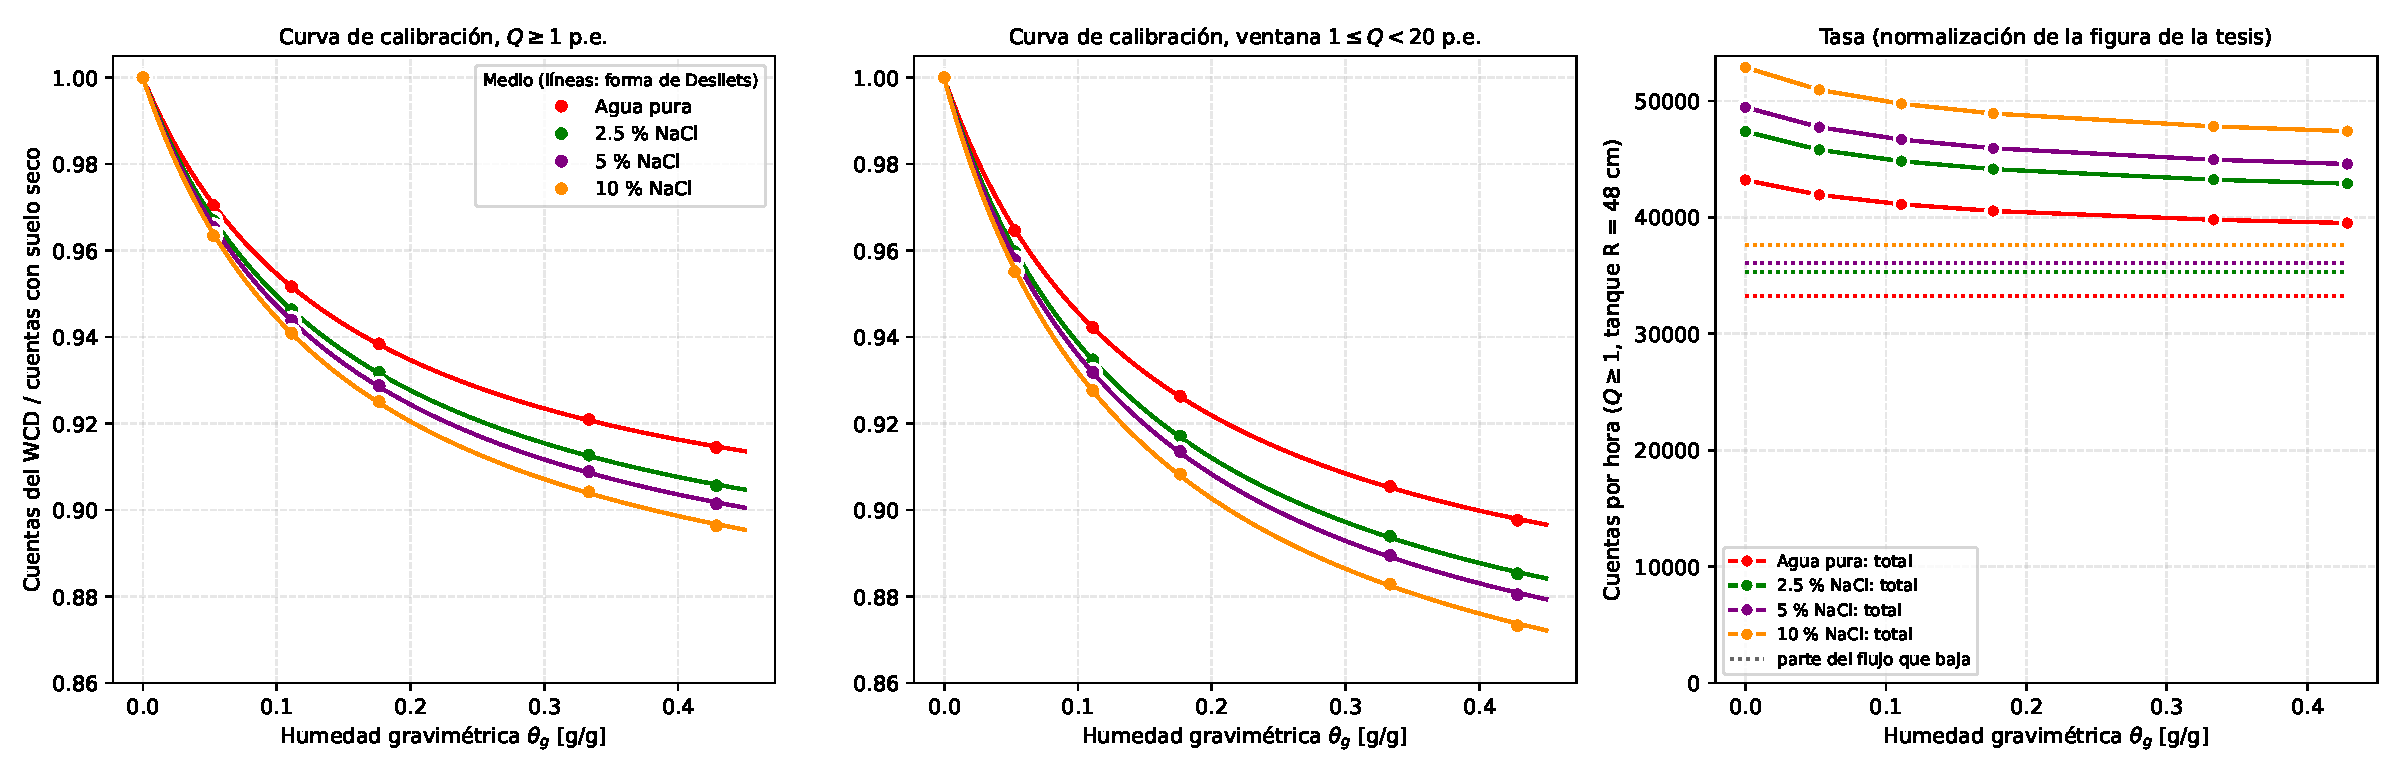
\includegraphics[width=\linewidth]{fig09_curva_calibracion_wcd.pdf}
\caption{Curva de calibración del WCD en los cuatro medios: $N/N_0$ frente a la humedad gravimétrica, con todo el
espectro, para $Q\geq1$~p.e.\ (izquierda) y con la ventana $1\leq Q<20$~p.e.\ (centro); las líneas son el ajuste de la
forma de Desilets. Derecha: cuentas por hora y, en puntos, la parte que viene del flujo que baja.}\label{fig:cal}
\end{figure}

\begin{itemize}
\item Entre el suelo seco y el 30~\% de agua, las cuentas bajan un \textbf{8.6~\%} en agua pura, 9.4~\% con 2.5~\%
NaCl, 9.9~\% con 5~\% y \textbf{10.4~\%} con 10~\% ($Q\geq1$): la sensibilidad crece con la sal. Con la ventana
$1\leq Q<20$~p.e., que descarta parte de las señales grandes de los neutrones de alta energía, la caída sube a 10.2, 11.5, 12.0 y
\textbf{12.7~\%}. La combinación NaCl + ventana es la más sensible.
\item Contando solo los neutrones de hasta 1~keV, la caída sería de 5--6~\%: la mayor parte de la señal está en los
neutrones rápidos.
\item La curva tiene la forma de Desilets, $N/N_0 = a_1 + a_0/(\theta_g + a_2)$. En agua pura,
$a_0 = 0.018$, $a_1 = 0.884$ y $a_2 = 0.157$; con NaCl y ventana, $a_0 = 0.026$, $a_1 = 0.829$ y $a_2 = 0.151$. El valor de
$a_1$ ($\approx0.85$, frente a 0.372 en Desilets et al.) refleja la fracción de cuentas que no depende del suelo.
\item Con la normalización de 12~h ($4.3\times10^4$, $4.7\times10^4$, $4.9\times10^4$ y $5.3\times10^4$ cuentas/h en agua pura y con 2.5, 5 y
10~\% NaCl, por plegado), la estadística de Poisson permite distinguir la humedad gravimétrica con $\sigma_{\theta_g}\approx0.006$--$0.009$
cerca del suelo seco y $\approx0.05$--$0.07$ con 30~\% de agua en una hora, y con $\approx0.0013$--$0.0017$ y
$\approx0.010$--$0.014$ en un día. Esa resolución escala como $1/\sqrt{\text{tasa}\times t}$; no incluye el fondo de
muones y de la componente electromagnética.
\end{itemize}

\subsection{Simulación directa en el tanque}\label{sec:directa}
El plegado usa la eficiencia de neutrones verticales que entran por la tapa. Para comprobarlo (esquema de la
figura~\ref{fig:esq3}) se inyectaron en el WCD
(SaltyWCD, PMT de Sidelnik a $0.3\,H/2$, sin suelo en la geometría) los neutrones que suben de cada suelo, con su
energía y su dirección reales: 100\,000 por suelo, en agua pura y con 2.5, 5 y 10~\% NaCl (paquete
\archivo{Corrida-tanque-albedo}; 26--50~min por corrida con 4 procesos).
\begin{itemize}
\item \textbf{Entrada.} El campo que sube es uniforme sobre el suelo, así que la tasa que entra por la base es
$J_\uparrow\pi R^2$ y la que entra por el costado $J_\uparrow\,2RH\,\langle\tan\theta\rangle$ ($R = 48.5$~cm,
$H = 135$~cm, $\theta$ el ángulo cenital de cada cruce del plano). Con el suelo seco llegan al tanque 41.9~n/s (12.3 por
la base y 29.6 por el costado); con 30~\% de agua, 28.8~n/s. El \textbf{71~\%} entra por el costado. Los cruces más rasantes
($\theta > 85^\circ$, que vienen de 25--40~m) se cortan; con 80$^\circ$ y sin corte la caída cambia menos de 0.4 puntos.
\item \textbf{Flujo que baja} (igual para todos los suelos). Por la tapa se toma del plegado (escalado a
$R = 48.5$~cm): 19.0~n/s. Por el costado entran 27.5~n/s ($\langle\tan\theta\rangle = 0.82$ en los 200\,000 neutrones que
bajan), con la eficiencia medida en los que suben por el costado. Esa eficiencia no cubre bien los neutrones de alta energía de más de
100~MeV, donde está la mayor parte del flujo que baja; como cota alta se usó la eficiencia vertical del plegado, que
da un 55~\% más de cuentas por el costado y una caída 1.3 puntos menor (el intervalo de la tabla~\ref{tab:dirres}).
\item \textbf{Estadística.} Unos 16\,000--26\,000 eventos con señal por corrida: 0.6--0.8~\% en las cuentas del flujo
que sube y $\approx0.3$ puntos en la caída.
\end{itemize}

\begin{figure}[H]\centering
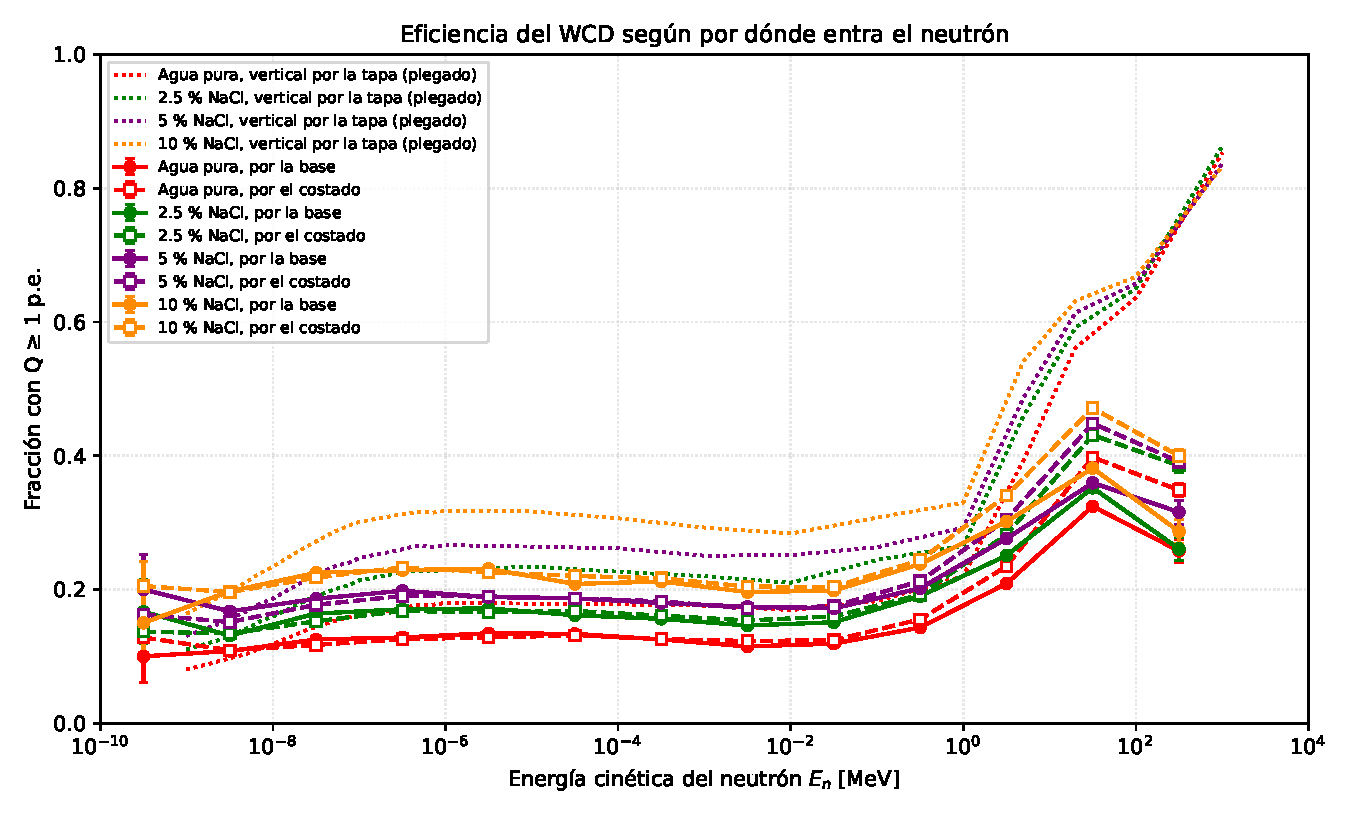
\includegraphics[width=0.85\linewidth]{fig14_eficiencia_base_costado.pdf}
\caption{Fracción de neutrones con $Q\geq1$~p.e.\ según su energía y por dónde entran al tanque: por la base (círculos)
y por el costado (cuadrados), en las corridas directas (las seis humedades juntas), frente a la eficiencia vertical por
la tapa que usa el plegado (puntos).}\label{fig:effbc}
\end{figure}

La eficiencia casi no depende de la humedad: 0.162--0.167 en agua pura, 0.198--0.205 con 2.5~\%, 0.220--0.228 con 5~\% y
0.254--0.260 con 10~\% NaCl, para todos los suelos. La base (0.157 en agua pura) y el costado (0.170) responden parecido entre sí, pero por debajo de 1~MeV quedan
un 25--30~\% por debajo de la incidencia vertical por la tapa (0.12--0.13 frente a 0.17--0.18 en agua pura). Por encima de
10~MeV la diferencia es mayor (0.35--0.40 frente a 0.56--0.85): los neutrones oblicuos recorren menos agua que los
verticales.

\begin{table}[H]
	\centering
	\caption{Simulación directa ($Q\geq1$~p.e.): cuentas por hora del flujo que baja (por la tapa y por el costado) y
		del que sube (por la base y por el costado), total y razón $N/N_0$, frente a la del plegado.}\label{tab:dir}	
	\footnotesize\setlength\tabcolsep{4pt}
\tabla{calibracion_directa}

\end{table}

\begin{table}[H]
	\centering
	\caption{Simulación directa frente al plegado: cuentas sobre el suelo seco, caída entre seco y 30~\% de agua con
		$Q\geq1$ (y su intervalo sistemático: corte rasante de 80$^\circ$ a sin corte y eficiencia del costado para el flujo
		que baja) y con la ventana $1\leq Q<20$~p.e., y la parte de las cuentas que viene del flujo que baja.}\label{tab:dirres}	
	\footnotesize\setlength\tabcolsep{4pt}
\tabla{calibracion_directa_resumen}

\end{table}

\begin{figure}[H]\centering
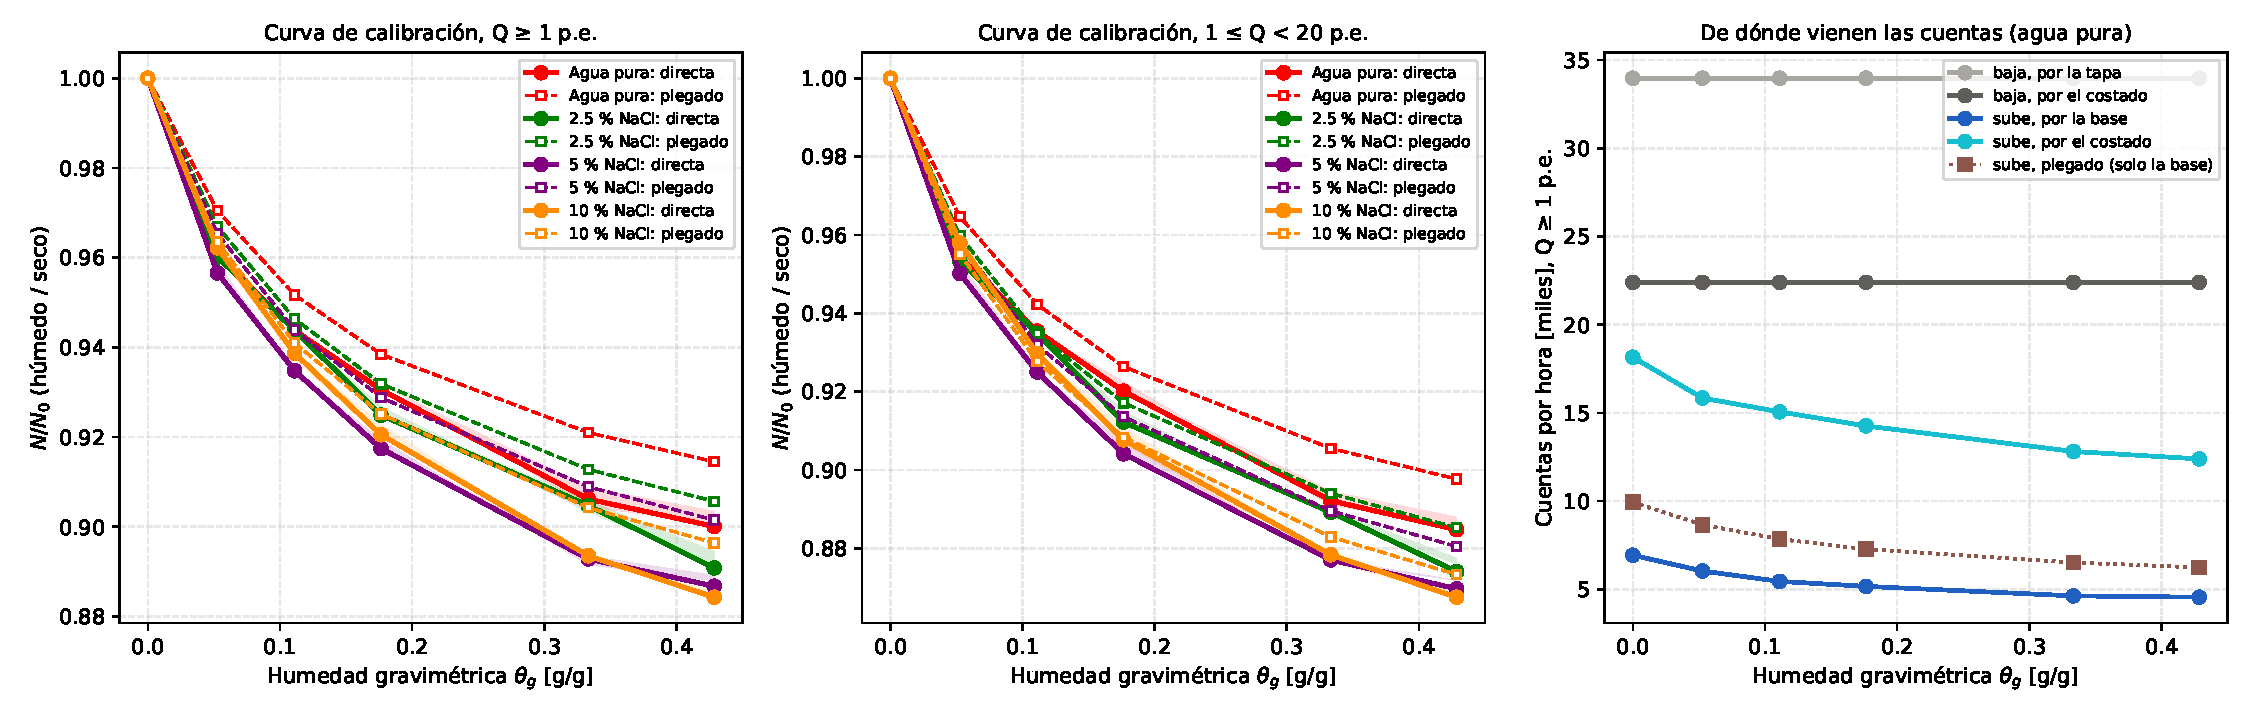
\includegraphics[width=\linewidth]{fig13_calibracion_directa.pdf}
\caption{Curva de calibración por simulación directa (círculos; la franja es el efecto del corte rasante) frente al
plegado (cuadrados), con $Q\geq1$~p.e.\ (izquierda) y con la ventana (centro). Derecha: cuentas por hora en agua pura
según la componente; en puntos, lo que el plegado asigna al flujo que sube.}\label{fig:dir}
\end{figure}

\begin{itemize}
\item Al sumar la entrada por el costado, las cuentas del flujo que sube son 2.5 veces las del plegado (25\,100
frente a 9\,940 por hora en agua pura, suelo seco), y las del total casi se duplican ($N_0 = 8.1\times10^4$ frente a
$4.3\times10^4$ cuentas/h). La parte que viene del flujo que baja pasa de 77 a 69~\% (agua pura), de 74 a 67~\% (2.5~\%), de 73 a
65~\% (5~\%) y de 71 a 64~\% (10~\% NaCl).
\item La caída entre seco y 30~\% de agua es de \textbf{10.0~\%} en agua pura (8.7--10.0~\% con los sistemáticos;
plegado 8.6~\%) y de \textbf{11.6~\%} con 10~\% NaCl (10.3--11.6~\%; plegado 10.4~\%); con 2.5 y 5~\% NaCl, 10.9 y 11.3~\% (plegado 9.4 y 9.9~\%). La caída crece de forma
monótona con la concentración, como en el plegado. Con la ventana, 11.5, 12.6, 13.0 y 13.2~\% (plegado 10.2, 11.5, 12.0 y
12.7~\%). Con $Q\geq5$~p.e. el NaCl conserva la sensibilidad (7.6, 9.2 y 10.0~\% con 2.5, 5 y 10~\%) y el agua pura la
pierde (2.9~\%), porque en agua pura casi no hay señales grandes.
\item El plegado subestima la sensibilidad en 1--1.5 puntos, pero reproduce la forma de la curva: la conclusión de la
sección anterior (NaCl y ventana aumentan la sensibilidad) no cambia. Ajuste de Desilets de la curva directa: $a_0 =
0.020$, $a_1 = 0.866$, $a_2 = 0.151$ (agua pura); $a_0 = 0.026$, $a_1 = 0.851$, $a_2 = 0.174$ (2.5~\%); $a_0 = 0.021$,
$a_1 = 0.849$, $a_2 = 0.142$ (5~\%) y $a_0 = 0.031$, $a_1 = 0.834$, $a_2 = 0.190$ (10~\% NaCl). Con seis puntos de
100\,000 neutrones, los tres parámetros se compensan entre sí y no deben leerse por separado; la caída y el promedio de la
sensibilidad (sección~\ref{sec:sens}) son las cantidades robustas.
\end{itemize}

\subsection{Sensibilidad a la humedad y resolución}\label{sec:sens}
La sensibilidad relativa del detector a la humedad se define como
\begin{equation}
	S_j(\theta_v) = -\frac{1}{R_j(\theta_v)}\,\frac{dR_j(\theta_v)}{d\theta_v},
\end{equation}
con $R_j = N_j/N_{0,j}$ la curva de calibración del medio $j$. Con los seis suelos ($\theta_v$ = 0, 0.124, 0.231, 0.323,
0.474 y 0.536) se ajustó a cada curva la forma de Desilets en $\theta_v$, $R = a_1 + a_0/(\theta_v + a_2)$ (residuos
menores que 0.0006 en el plegado y de 0.001 a 0.005 en la simulación directa, por su estadística), y se derivó el ajuste.
La resolución estadística en humedad es $\sigma_{\theta_v} = \sqrt{N}/|dN/d\theta_v|$, con $N = R_j N_{0,j}\,t$ y la
normalización de 12~h. Como comprobación, el promedio de $S_j$ en todo el intervalo coincide con
$-\ln R_j/\theta_v$ evaluado con 30~\% de agua.

\begin{figure}[H]\centering
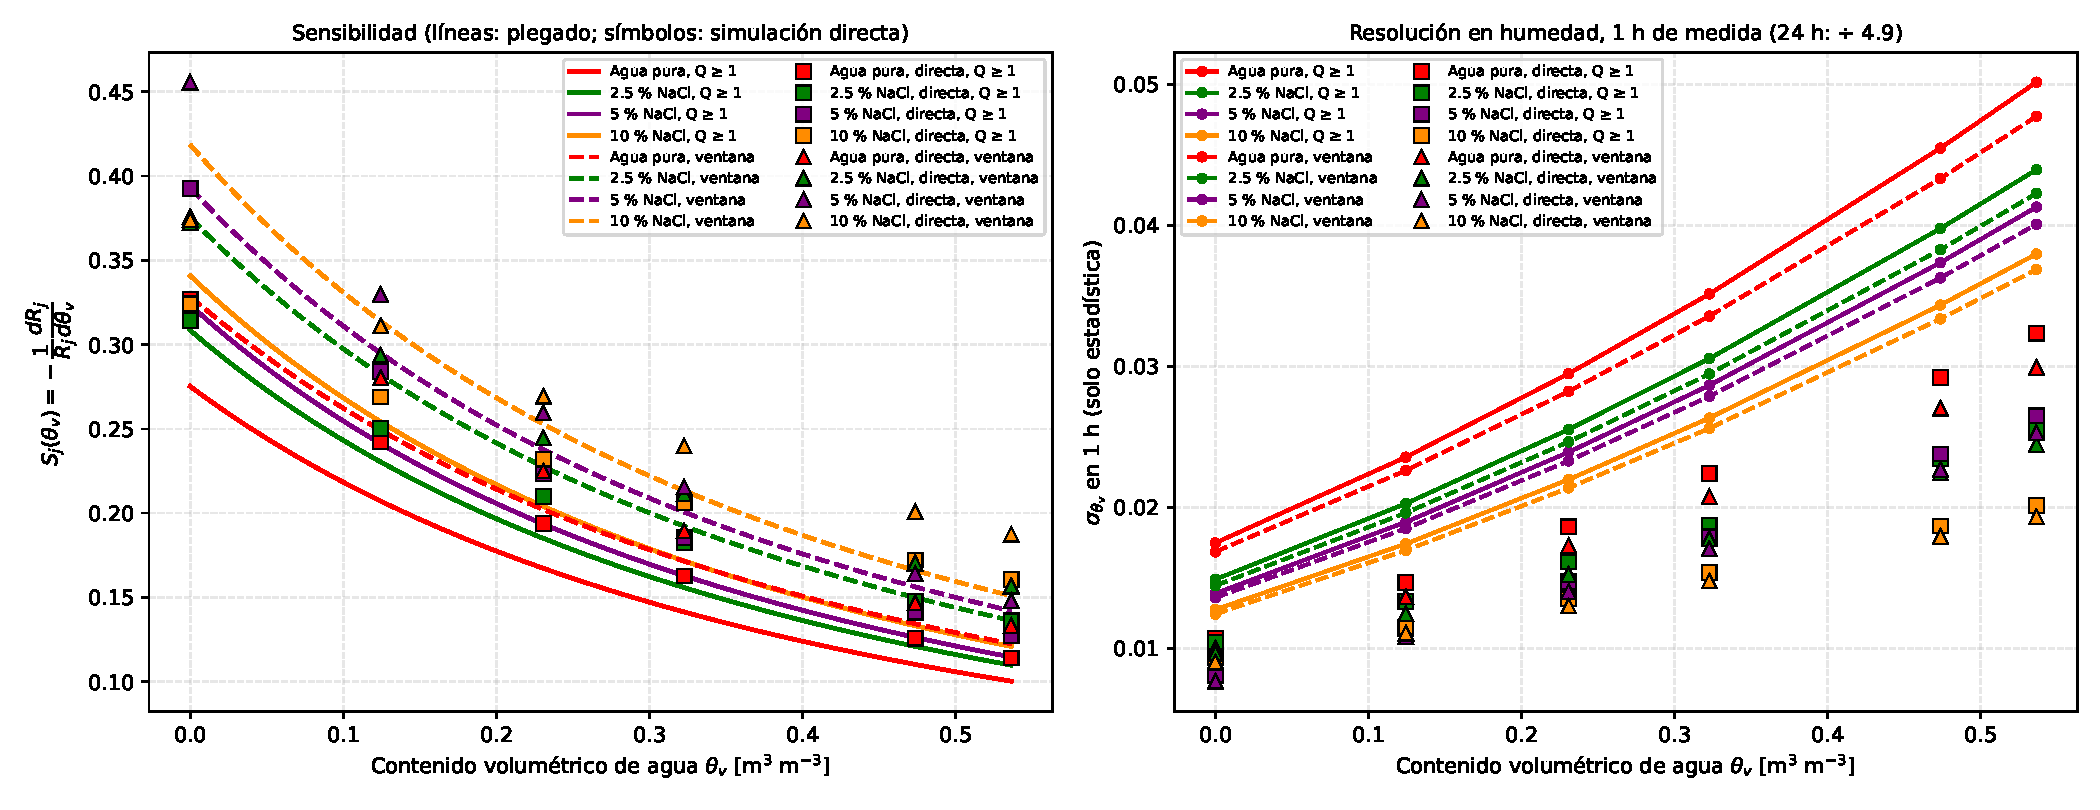
\includegraphics[width=\linewidth]{fig25_sensibilidad.pdf}
\caption{Izquierda: sensibilidad $S_j(\theta_v)$ por plegado (líneas; continuas $Q\geq1$, a trazos ventana
$1\leq Q<20$~p.e.) y por simulación directa (símbolos). Derecha: resolución estadística en humedad para 1~h de medida
(para 24~h, dividir por 4.9).}\label{fig:sens}
\end{figure}

\begin{table}[H]
	\centering
	\caption{Sensibilidad $S_j$ en el suelo seco, con 30~\% de agua y en promedio, y resolución estadística
		$\sigma_{\theta_v}$ en 1 y 24~h, por plegado y por simulación directa, con $Q\geq1$ y con la ventana.}\label{tab:sens}	
	\footnotesize\setlength\tabcolsep{4pt}
\tabla{sensibilidad}

\end{table}

\begin{itemize}
	\item La sensibilidad es mayor en el suelo seco y baja unas tres veces hasta 30~\% de agua, como corresponde a la forma de
	Desilets: el detector distingue mejor los cambios de humedad en suelos secos.
	\item El NaCl sube la sensibilidad media un 11, 16 y 22~\% con 2.5, 5 y 10~\% de sal (0.185, 0.193 y 0.204 frente a
	0.167 con $Q\geq1$, por plegado) y la
	ventana de carga otro 20~\%; juntos, 0.253, un 52~\% más que el agua pura con $Q\geq1$.
	\item La configuración con 10~\% de NaCl y ventana combina la pendiente más alta con la tasa más alta y tiene la mejor
	resolución: $\sigma_{\theta_v}\approx0.012$ (seco) y 0.037 (30~\%) en 1~h por plegado, y 0.009 y 0.019 en la simulación
	directa; en 24~h, 0.0025--0.0075 y 0.0018--0.0039. Con 2.5 y 5~\% y ventana, 0.015/0.042 y 0.014/0.040 en 1~h
	por plegado.
	\item La simulación directa, que incluye la entrada por el costado, da algo más de sensibilidad que el plegado. Su
	promedio crece con la sal igual que en el plegado: 0.196, 0.216, 0.224 y 0.229 con $Q\geq1$ y 0.228, 0.251, 0.260 y
	0.265 con la ventana (agua pura, 2.5, 5 y 10~\% NaCl). Los valores punto a punto (en el seco y con 30~\%) dependen de
	un ajuste a seis puntos con ruido estadístico y no siguen un orden limpio entre los medios.
	\item Son cotas superiores: solo hay neutrones. El fondo de muones y de la componente electromagnética, que no depende de
	la humedad, bajaría $S_j$ y empeoraría $\sigma_{\theta_v}$; tampoco se incluyen la transparencia y la estabilidad del
	medio.
\end{itemize}

\subsection{Limitaciones}\label{sec:lim}
\begin{enumerate}
\item \textbf{Normalización absoluta.} El archivo \archivo{all_bga_neutron_35.shw} equivale a 1~m$^2$ y 12~h, verificado
con la corrida de ARTI de 300~s a 956~m (sección~1). Ese flujo de ARTI es el de CORSIKA para la rigidez de Bucaramanga
(11.6~GV); queda por compararlo con medidas en el sitio. Las razones $N/N_0$ no dependen de la normalización; la tasa y
la resolución sí.
\item \textbf{Incidencia.} El plegado usa neutrones verticales por la tapa. La simulación directa
(sección~\ref{sec:directa}) mide la entrada por la base y por el costado del flujo que sube; el flujo que baja por el
costado se estima con la eficiencia del costado de los que suben, con una cota alta por la vertical.
\item \textbf{Tanque a 2~m del suelo.} El campo se toma a 5~cm del suelo; en los 2~m de aire casi no cambia, pero no
se simuló.
\item \textbf{Solo neutrones.} El WCD real también cuenta muones y la componente electromagnética, que no dependen de la
humedad y diluyen más la señal. Separarlos (ventana de tiempo de la captura, carga del Cl con NaCl) es parte del método
de la tesis.
\end{enumerate}

\section{Conclusiones}
\begin{enumerate}
\item El suelo seco de MEIGA reproduce el espectro seco de la tesis por debajo de 10~MeV; por encima queda un 25~\% más
bajo, por diferencias entre las dos simulaciones.
\item Con la clasificación de la tesis, y con el mismo montaje y los mismos neutrones, la humedad reduce los
intermedios a \IntTreinta{} y los rápidos a \RapTreinta{} con 30~\% de agua, los epitérmicos solo a \EpiTreinta, y
sube los térmicos un 42~\%. El albedo total pasa de \albSeco{} a \albTreinta.
\item Cada investigación de CRNS delimita las energías a su manera; la ventana de sus detectores (10~eV--1~keV a
0.1--10~keV) cae en los intermedios de la tesis, mientras que la banda más sensible para el WCD (0.1--3~MeV) está en
los rápidos.
\item La caída sigue la forma de Desilets con parámetros propios; con los de la literatura, los intermedios difieren
hasta 0.05.
\item Dentro del suelo, el agua duplica las colisiones elásticas del neutrón incidente, reduce de 3.4 a 2.2 los
neutrones creados por neutrón inyectado (menos evaporación) y hace del hidrógeno el núcleo que más captura (66~\% con
30~\% de agua).
\item La banda de 10~meV a 10~eV es casi insensible a la humedad (\bandaMax~\%); el tanque debe recibir el espectro
completo.
\item Plegando los espectros con la eficiencia del WCD de 1~meV a 1~GeV, las cuentas bajan entre el suelo seco y el
30~\% de agua un 8.6, 9.4, 9.9 y 10.4~\% (agua pura y 2.5, 5 y 10~\% NaCl); con la ventana $1\leq Q<20$~p.e., 10.2,
11.5, 12.0 y 12.7~\%. La curva
sigue la forma de Desilets. Tres cuartas partes de las cuentas vienen del flujo que baja, que no depende del suelo: el
NaCl y la ventana de carga son las dos maneras de aumentar la sensibilidad.
\item El coeficiente de captura del neutrón incidente crece de 17.4~\% (1~meV) a una meseta de 35--36~\% en los
epitérmicos y a un máximo de 62.8~\% en 5~MeV (agua pura); con 2.5~\%, de 20.6 a 41 y 65.6~\%; con 5~\%, de 23.4
a 45 y 66.6~\%, y con 10~\% NaCl, de 28.1 a 51 y 68.8~\%. Desde 20~MeV el
neutrón incidente casi no se captura: domina la interacción inelástica (53--81~\%) y la transmisión (hasta 24~\%). El NaCl aumenta la captura hasta 1.6 veces, a costa de la
reflexión por la tapa, que baja de 76.6 a 62.2~\% (1~meV a 1~eV) en agua pura, de 73.3 a 57.2~\% con 2.5~\%, de
70.5 a 53.1~\% con 5~\% y de 66.0 a 46.8~\% con 10~\% NaCl.
\item La simulación directa en el tanque, con los neutrones que suben entrando por la base y por el costado (71~\% por
el costado), da una caída algo mayor que el plegado: 10.0, 10.9, 11.3 y 11.6~\% en agua pura y con 2.5, 5 y 10~\% NaCl (8.6,
9.4, 9.9 y 10.4~\% en el plegado), y de 11.5 a 13.2~\% con la ventana. El plegado es una estimación conservadora de la sensibilidad y conserva
la forma de la curva.
\end{enumerate}
\ifquince\else\aviso{Pendiente: la corrida con 15~\% de agua, en el tramo donde más cambia la curva. Al agregarla a
\archivo{analizar_albedo.py} y volver a correr \archivo{curva_humedad.py}, las tablas, las figuras y las cifras de este
informe se actualizan solas.}\fi

\begin{sloppypar}
\paragraph{Reproducción.} Todo el informe se rehace desde \archivo{Albedo-suelo-humedo/} con
\archivo{scripts/actualizar_informe.sh [carpeta de las corridas]}. El script busca las corridas del suelo en el
disco, corre \archivo{analizar_albedo.py} (corridas completas y mismos neutrones), \archivo{curva_humedad.py},
\archivo{procesos_neutrones.py}, \archivo{graficas_espectros.py}, \archivo{curva_calibracion_wcd.py},
\archivo{balance_rapidos.py}, \archivo{captura_wcd.py}, \archivo{luz_barrido.py}, \archivo{sensibilidad.py} y
\archivo{curva_calibracion_tanque.py} (resultados del paquete \archivo{Corrida-tanque-albedo}, variable
\archivo{TANQUE_RES}), y compila el informe. Las eficiencias de 1~keV a 1~GeV vienen del paquete \archivo{Barrido-rapidos-WCD}
(\archivo{resultados/eficiencias_rapidos.tsv}); las de 1~meV a 1~keV, de la Campaña~1 en el repositorio de la tesis.
Las regiones de energía están definidas una sola vez, en \archivo{scripts/regiones.py}.
\end{sloppypar}

\begin{thebibliography}{9}
\bibitem{Arti2022} C.~Sarmiento-Cano, M.~Suárez-Durán, R.~Calderón-Ardila, A.~Vásquez-Ramírez, A.~Jaimes-Motta,
L.~A.~Núñez, S.~Dasso, I.~Sidelnik y H.~Asorey, ``The ARTI framework: cosmic rays atmospheric background simulations'',
\emph{The European Physical Journal C} \textbf{82}(11), 1019 (2022).
doi:\href{https://doi.org/10.1140/epjc/s10052-022-10883-z}{10.1140/epjc/s10052-022-10883-z}; preprint arXiv:2010.14591.
\bibitem{Asorey2018} H.~Asorey, L.~A.~Núñez y M.~Suárez-Durán, ``Preliminary results from the Latin American Giant
Observatory space weather simulation chain'', \emph{Space Weather} (2018).
doi:\href{https://doi.org/10.1002/2017SW001774}{10.1002/2017SW001774}; preprint arXiv:1802.08867 (ecs.~13--14).
\bibitem{SarmientoCano2025repo} C.~Sarmiento-Cano, \emph{ReunionLAGO2025\_ARTI}, repositorio del taller de ARTI (2025),
\url{https://github.com/csarmiento03/ReunionLAGO2025_ARTI} (archivos \texttt{Salida\_BGA\_300.shw} y \texttt{.hst};
consultado el 26 de octubre de 2026).
\bibitem{Desilets2010} D.~Desilets, M.~Zreda y T.~P.~A.~Ferré, ``Nature's neutron probe: Land surface hydrology at
an elusive scale with cosmic rays'', \emph{Water Resources Research} \textbf{46}(11), W11505 (2010).
doi:\href{https://doi.org/10.1029/2009WR008726}{10.1029/2009WR008726}.
\bibitem{Desilets2013} D.~Desilets y M.~Zreda, ``Footprint diameter for a cosmic-ray soil moisture probe: Theory and
Monte Carlo simulations'', \emph{Water Resources Research} \textbf{49}(6), 3566--3575 (2013).
doi:\href{https://doi.org/10.1002/wrcr.20187}{10.1002/wrcr.20187}.
\bibitem{IAEA2023Cold} International Atomic Energy Agency, \emph{Cold Neutron Sources: Practical Considerations and
Modern Research}, IAEA-TECDOC-2025, IAEA, Viena (2023). ISBN 978-92-0-139423-1.
\bibitem{Kohli2015} M.~Köhli, M.~Schrön, M.~Zreda, U.~Schmidt, P.~Dietrich y S.~Zacharias, ``Footprint
characteristics revised for field-scale soil moisture monitoring with cosmic-ray neutrons'', \emph{Water Resources
Research} \textbf{51}(7), 5772--5790 (2015). doi:\href{https://doi.org/10.1002/2015WR017169}{10.1002/2015WR017169};
preprint arXiv:1602.04469.
\bibitem{Kohli2018} M.~Köhli, M.~Schrön y U.~Schmidt, ``Response functions for detectors in cosmic ray neutron
sensing'', \emph{Nuclear Instruments and Methods in Physics Research A} \textbf{902}, 184--189 (2018).
doi:\href{https://doi.org/10.1016/j.nima.2018.06.052}{10.1016/j.nima.2018.06.052}; preprint arXiv:1801.07997.
\bibitem{Krane1988} K.~S.~Krane, \emph{Introductory Nuclear Physics}, John Wiley \& Sons, Nueva York (1988).
ISBN 978-0-471-80553-3.
\bibitem{Podgorsak2010} E.~B.~Podgoršak, \emph{Radiation Physics for Medical Physicists}, 2.ª ed., Springer, Berlín
(2010). doi:\href{https://doi.org/10.1007/978-3-642-00875-7}{10.1007/978-3-642-00875-7}.
\bibitem{Sidelnik2020} I.~Sidelnik, H.~Asorey, N.~Guarín, M.~Suárez Durán, M.~Gómez Berisso, J.~Lipovetzky y
J.~J.~Blostein, ``Simulation of 500 MeV neutrons by using NaCl doped water Cherenkov detector'', \emph{Advances in Space
Research} \textbf{65}(9), 2216--2222 (2020). doi:\href{https://doi.org/10.1016/j.asr.2020.02.024}{10.1016/j.asr.2020.02.024}.
\bibitem{Zreda2012} M.~Zreda, W.~J.~Shuttleworth, X.~Zeng, C.~Zweck, D.~Desilets, T.~Franz y R.~Rosolem, ``COSMOS:
the COsmic-ray Soil Moisture Observing System'', \emph{Hydrology and Earth System Sciences} \textbf{16}(11),
4079--4099 (2012). doi:\href{https://doi.org/10.5194/hess-16-4079-2012}{10.5194/hess-16-4079-2012}.
\end{thebibliography}
\noindent\small Las claves de las referencias son las de \archivo{bibliografia-1.bib} de la tesis; solo
\texttt{Desilets2013} es nueva. Las secciones citadas de~\cite{Kohli2015,Kohli2018} se verificaron en los preprints de
arXiv; las páginas impresas de esas frases no. De~\cite{Desilets2013} solo se consultó el resumen. Krane, Podgoršak e
IAEA se citan como en la Tabla~2.2 de la tesis.

\end{document}
